\chapter{Shower shapes corrections}
\label{ch:ss_corrections}
\epigraph{\emph{“Champions keep playing until they get it right.”}}{Billie Jean King}


In the previous chapter, it was seen that \acp{SF} (ratio of data efficiencies to simulated ones) deviate from unity. Given that photon identification relies on cuts to the photon \acp{SS}, it was found that the differences in fact appear on these variables. Since Run-1, they have been corrected with what is known as \acfp{FF}, which, historically, they have been computed as simple shifts to the \ac{MC} distributions and have been found to provide very good improvements on the \acp{SF}. However, as seen before, there are still discrepancies between the distributions that need to be addressed in order to rely on even a better simulation.
In \Sect{\ref{sec:ss_corrections:ffs}}, a more sophisticated approach based on a higher order computation to correct the \acp{SS} is presented. Also, a novel approach using directly the cells energies is studied and addressed in \Sect{\ref{sec:ss_corrections:cell_rw}}. The studies presented in this chapter comprise one of the main topics of work for the current thesis.





\section{\acfp{FF}}
\label{sec:ss_corrections:ffs}


\subsection{Data and simulated samples}
\label{subsec:ss_corrections:ffs:samples}

\acp{FF} are computed using full Run-2 dataset, collected at \(\sqrt{s}=13~\tev\) and with a corresponding integrated luminosity of \(140~\ifb\).
Both the \ac{RZ} and \ac{SP} simulated samples are used for this study, as their represent complementary \pt-ranges. \ac{RZ} events are generated with \SHERPA 2.2.11~\cite{Sherpa2.2}, while \SHERPA 2.2.1 is used for \(\Zboson \to \ell\ell\) background events. Respecting the \ac{SP} samples, events are generated with \PYTHIA 8.186~\cite{Pythia8.1}, which includes leading-order \gammajet events from both direct processes (\(qg\to q\gamma\) and \(\qqbar \to g \gamma\)) and photon fragmentation from \ac{QCD} dijet events.

In both cases, the \ac{ATLAS} detector is simulated using \GEANT 4~\cite{Geant4} and the \ac{MC} events are reweighted so that their pileup distributions resembles the one in data, for each year of the Run-2 data-taking period.


\subsection{Calculation}
\label{subsec:ss_corrections:ffs:calculation}

% \acp{FF} are computed in a series of steps that start by preparing the input datasets up to the systematic uncertainties calculation. In the first step, histograms of all the \acp{SSV} are created and then smoothed, which are then used to perform the actual optimisation of the \acp{FF}.
% % This process is repeated for different isolation and identification selection requirements, in order to compute the systematic uncertainties.
% In the following a step by step description of the process is described.

The calculation is performed separately for the two considered samples: \ac{RZ} for photons with \(7\leq\pt\leq 50~\gev\) and \ac{SP} for photons with \(\pt> 50~\gev\), which were already discussed in \Sect{\ref{subsec:pid_ss:pid:event_selection}}. Since \acp{SS} distributions vary as a function of \pt and \abseta, the computation is done in bins of these variables:
\begin{gather}
    \ptgam:
    \begin{cases}
        \text{\ac{RZ}}: [7,\, 15,\, 20,\, 30,\, 50] ~\gev\\
        \text{\ac{SP}}: (50,\, 60,\, 80,\, 100,\, 150,\, 300,\, 600,\, \infty] ~\gev\\
    \end{cases}\\
    \abseta: [0,\, 0.6,\, 0.8,\, 1.15,\, 1.37,\, 1.52,\, 1.81,\, 2.01,\, 2.37].
\end{gather}
Furthermore, as mentioned in \Sect{\ref{sec:pid_ss:ss}}, there are variables very sensitive to the photon's conversion status, that is, whether if the photons are converted or unconverted. For this reason, the calculation is done separately for converted and unconverted photons. A total of nine variables are corrected using this method: \eratio, \fside, \reta, \rphi, \rhad, \rhado, \wone, \weta and \wstot; as they are the ones in which the largest discrepancies are observed between data and \ac{MC}.

For each \ac{SS}, histograms of \ac{MC} and data of 100 bins are created. The choice of the binning is done based on having sufficient statistics at each bin and also to capture all the features of the variables.
After that, each histogram is smoothed using the \acf{KDE} tool from TMVA~\cite{TMVA}. The \ac{KDE} method consists of estimating the shape of a \acf{PDF2} by the sum over smeared events. The \ac{PDF2} \(p(x)\) of a variable \(x\) is
\begin{equation}
	p(x) = \frac{1}{N}\sum_{i=1}^{N} K_h(x-x_i)
\end{equation}
where \(N\) is the number of events, \(K_h(t) = K(t/h)/h\) is the kernel function, and \(h\) is the bandwidth of the kernel. The basic idea is that each event is considered as a Dirac-\(\delta\)-function, which is replaced by a Kernel function (Gaussian) and finally they are summed altogether to form the final \ac{PDF2}. The \ac{KDE} smoothing can be applied in two forms: non-adaptive \ac{KDE} or adaptive \ac{KDE}, as seen in \Fig{\ref{fig:ss_corrections:ffs:calculation:adaptive_nonadaptive_kde}}. In the former, the bandwidth is constant for the entire sample \(h_{NA}\), while in the latter, it uses the value from non-adaptive \ac{KDE}, but it varies as a function of \(p(x)\) as
\begin{equation}
	h_A = \frac{h_{NA}}{\sqrt{p(x)}}
\end{equation}
Adaptive \ac{KDE} improves the shape of the estimated \ac{PDF2} in regions of low statistics, however, in high statistics regions it can give rise to over-smoothing. The degree of smoothing is tuned by multiplying the bandwidth \(h\) by fine factors. 
These fine factors are user-defined parameter which are tuned to allow the \ac{PDF2} to retain the important features of the \ac{SS} but to also avoid statistical fluctuations. Higher values indicate broader Kernel functions and therefore de \ac{PDF2} catches less statistical fluctuations.
Examples of the smoothing procedure applied to \rhad are shown in \Fig{\ref{fig:ss_corrections:ffs:calculation:smoothing_ss}} for cases in which original histograms have low and high statistics.

\begin{figure}[ht!]
    \centering
    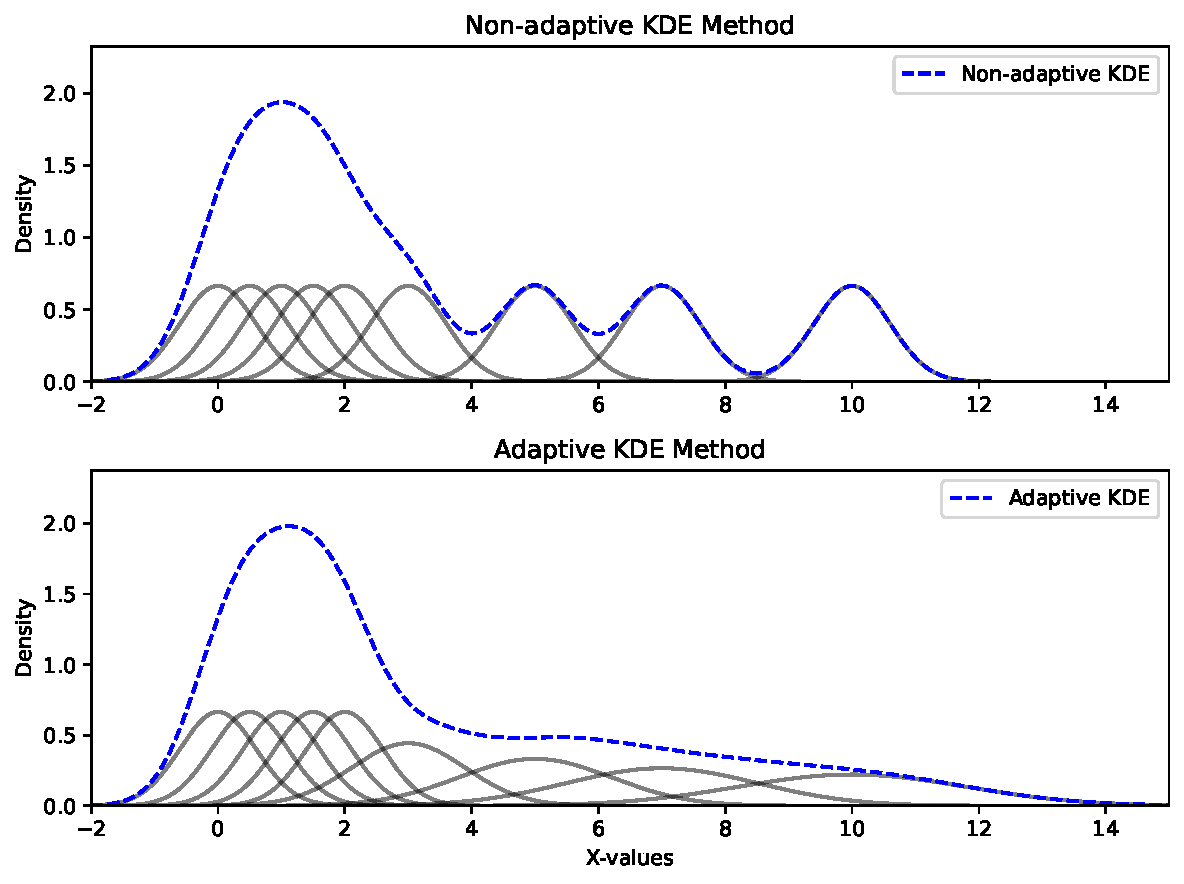
\includegraphics[width=0.6\linewidth]{4_photonid/ffs/smoothing/kde}
    \caption{Adaptive and non-adatptive \ac{KDE} smoothing.}
    \label{fig:ss_corrections:ffs:calculation:adaptive_nonadaptive_kde}
\end{figure}

\begin{figure}[ht!]
    \centering
    \begin{subfigure}[h]{0.49\linewidth}
        \centering
        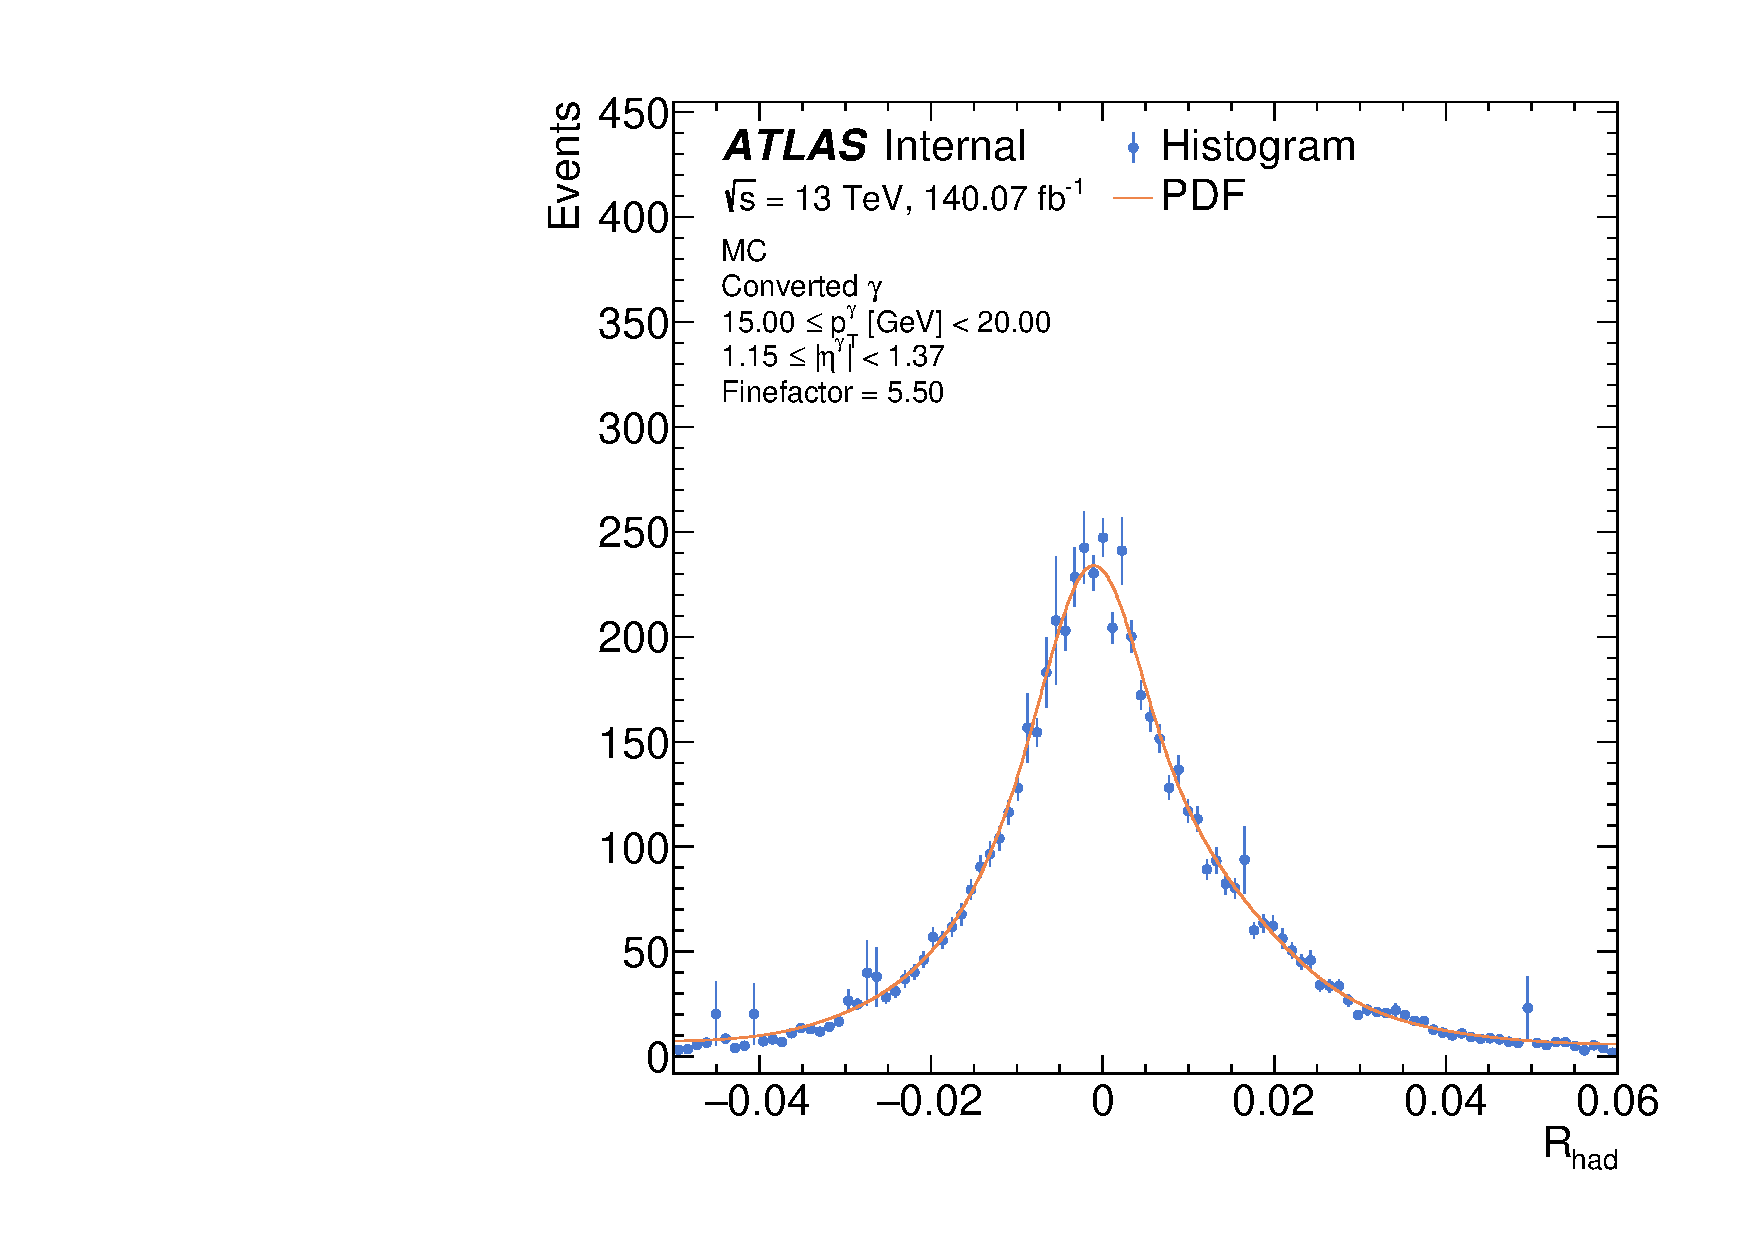
\includegraphics[width=\linewidth]{4_photonid/ffs/smoothing/can__pdfhist__mc__ph_rhad1__c_pt15p0_eta1p15}
        \caption{Low statistics case: \ac{RZ}}
    \end{subfigure}
    \hfill
    \begin{subfigure}[h]{0.49\linewidth}
        \centering
        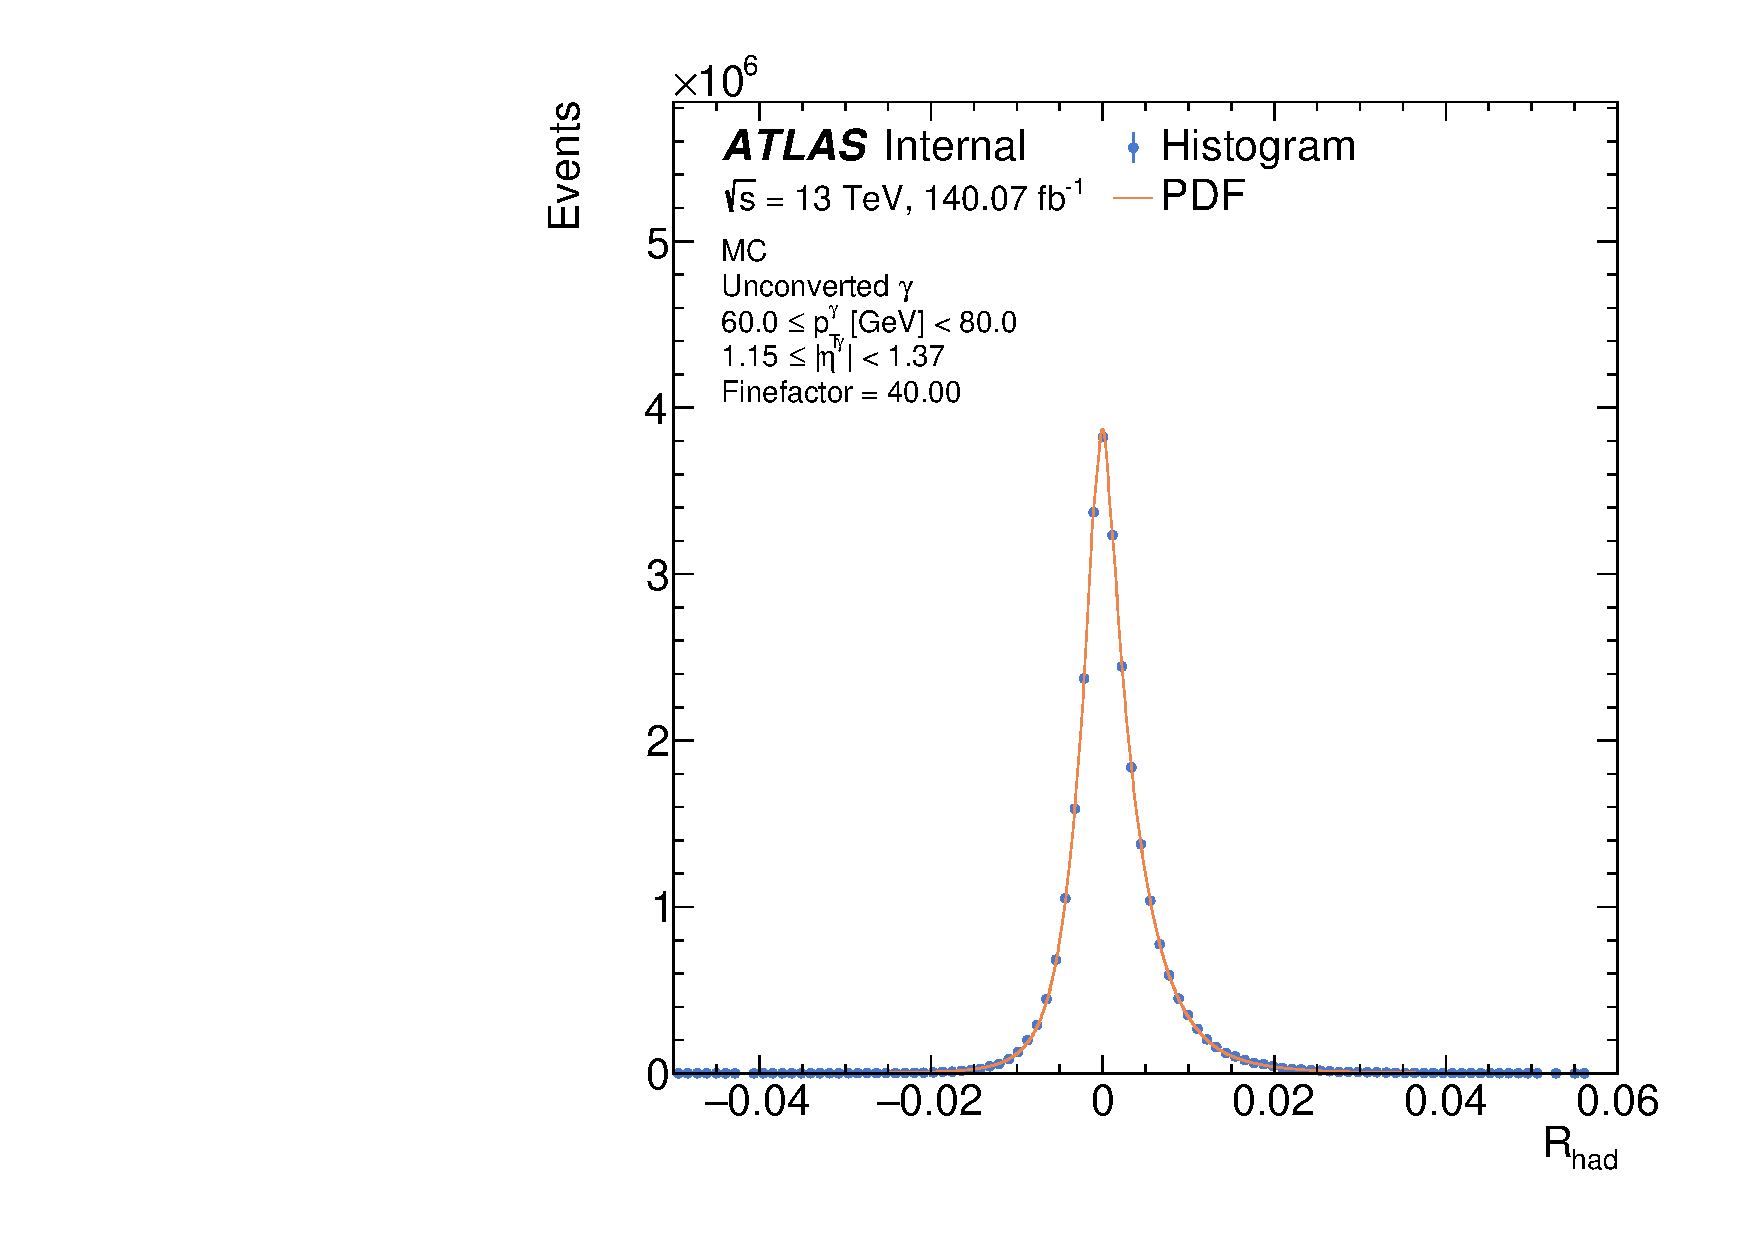
\includegraphics[width=\linewidth]{4_photonid/ffs/smoothing/can__pdfhist__mc__ph_rhad1__u_pt0060p0_eta1p15}
        \caption{High statistics case: \ac{SP}}
    \end{subfigure}
    \caption{\ac{KDE} smoothing applied to the \rhad for photons in \(0.8<\abseta<1.15\) in two scenarios: low and high statistics. Original histograms are shown with the blue points and their \acp{PDF2} with the orange lines. The fine factors used for each case are displayed in the figure.}
    \label{fig:ss_corrections:ffs:calculation:smoothing_ss}
\end{figure}


Once the data and \ac{MC} \acp{PDF2} are created for a given variable, \pt, \abseta and conversion type, the \ac{MC} \ac{PDF2} is normalised to data's and a \chisq value is computed between both, excluding the underflow and overflow bins, as:
\begin{equation}
	\chisq = \sum_{i=1}^{N} \dfrac{(w_{\text{MC},i} W_{\text{data}} - w_{\text{data},i} W_{\text{MC}})^2}{s_{\text{MC},i}^2 W_{\text{data}}^2 + s_{\text{data},i}^2 W_{\text{MC}}^2}.
\end{equation}
\(N\) is the number of bins in the \acp{PDF2}, \(w_{\text{MC},i}\) and \(w_{\text{data},i}\) are the event numbers of \ac{MC} and data at each bin, respectively, \(s_{\text{MC},i}\) and \(s_{\text{data},i}\) are the bin errors and finally \(W_{\text{data}}\) and \(W_{\text{MC}}\) are the sum of weights for data and \ac{MC}, respectively.

\subsubsection{Shift-only corrections}

Taking into account only the mean's correction of the \acp{SS}, the \ac{MC} \ac{PDF2} is shifted to the left and right one bin at a time. As a consequence of this procedure, the shift \ac{FF} resolution directly depends on the bin-width of the \acp{PDF2}, therefore having smaller bin-widths mean to obtain a better resolution on the shift value. Given that histograms, in the first place, are built with relative wide bins, the \acp{PDF2} can be constructed using high-accuracy narrow bin to ensure high resolution. After convergence tests on the \acp{FF}, the \acp{PDF2} are constructed with 5000 bins.
The starting number of bins that the \ac{MC} distribution needs to be shifted is estimated by computing the difference on the means between data and simulation. From this starting value, shifts of 100 bins to each side are considered.

For each bin the distribution has been shifted, the aforementioned \chisq value is computed and recorded. Assuming that the measurements errors \(s_{\text{MC},i}\) and \(s_{\text{data},i}\) have a normal gaussian distribution~\footnote{This requirement is satisfied as long as the bin contents of both \acp{PDF2} are greater than 10, which is also satisfied since histograms are built with relatively wide bins.}, and that the parameters for each \(\chi^2\) value are independent, it is expected that the shape followed by the \chisq values is approximately paraboloidal.

To extract the \acp{FF}, the \chisq scan near the minimum is fitted with a parabolic function (5 bins to each side of the minimum bin) and the shift \ac{FF} is obtained from the fit minimum. Finally, the \acp{SS} can be corrected as
\[
	\text{SS}_{\text{new}} = \text{SS}_{\text{old}} + \text{shift}.
\]


\subsubsection{Shift+stretch corrections}

It was seen that even after applying corrections to the means of the \ac{MC} \acp{SS} distributions, differences remained on the shapes of them, and in some cases these can be quite substantial. One way to continue improving the agreement between data and \ac{MC} is to include another correction which is referred as \textit{stretching}. The two corrections, called shift+stretch corrections, are meant to fix both the mean and the widths of the \ac{MC} distributions simultaneously.

The shift+stretch correction method starts by finding the maximum of the \ac{MC} \ac{PDF2}. The \ac{PDF2} is then stretched around it by calculating the new position of each bin by the product: \(\text{stretch}\times (x - \text{stretch point})\). In this manner, each bin's center conserves the initial distance to the center of the distribution, multiplied by the stretch factor. In the scenario where the shift is \(>1\), there might be cases in which it is big enough to give rise to empty bins inbetween. The content of these empty bins are then linearly interpolated from the neighbouring non-zero bins.
Once the \ac{PDF2} is stretched, it is then shifted left and right following the same procedure as for the shift-only case, calculating \chisq values for each \(\text{shift}_i\) after applying \(\text{stretch}_j\). As a result of the precedure, now, a two-dimensional grid on the shift-stretch plane of \chisq values is obtained. The pair of shift-stretch \acp{FF} is now retrieved from the minimum bin's center, and the corrections are applied to the \ac{MC} \acp{SS} as:
\begin{equation}
	\text{SS}_{\text{new}} = \text{stretch}\times(\text{SS}_{\text{old}} - \text{stretch point}) + \text{shift} + \text{stretch point}.
\end{equation}

An example of the resulting \chisq values for the \fside variable for unconverted photons with \(15<\pt<20~\gev\) in \(2.01<\abseta<2.37\) is shown in \Fig{\ref{fig:ss_corrections:ffs:calculation:fside_calculation:chi2}}, where the shift is on the \(x\)-axis and the stretch on the \(y\)-axis. The optimal shift-stretch value is given be the position of the minimum bin, which corresponds to \(\text{shift}=0.03\) and \(\text{stretch}=1.09\). A visualisation of the \acp{PDF2} before and after applying the corrections is shown in \Fig{\ref{fig:ss_corrections:ffs:calculation:fside_calculation:pdfs}}, where they are compared with the data distribution. As seen from the figure, there is a huge improvement and the distributions match almost perfectly.

\begin{figure}[ht!]
    \centering
    \begin{subfigure}[t]{0.49\linewidth}
        \centering
        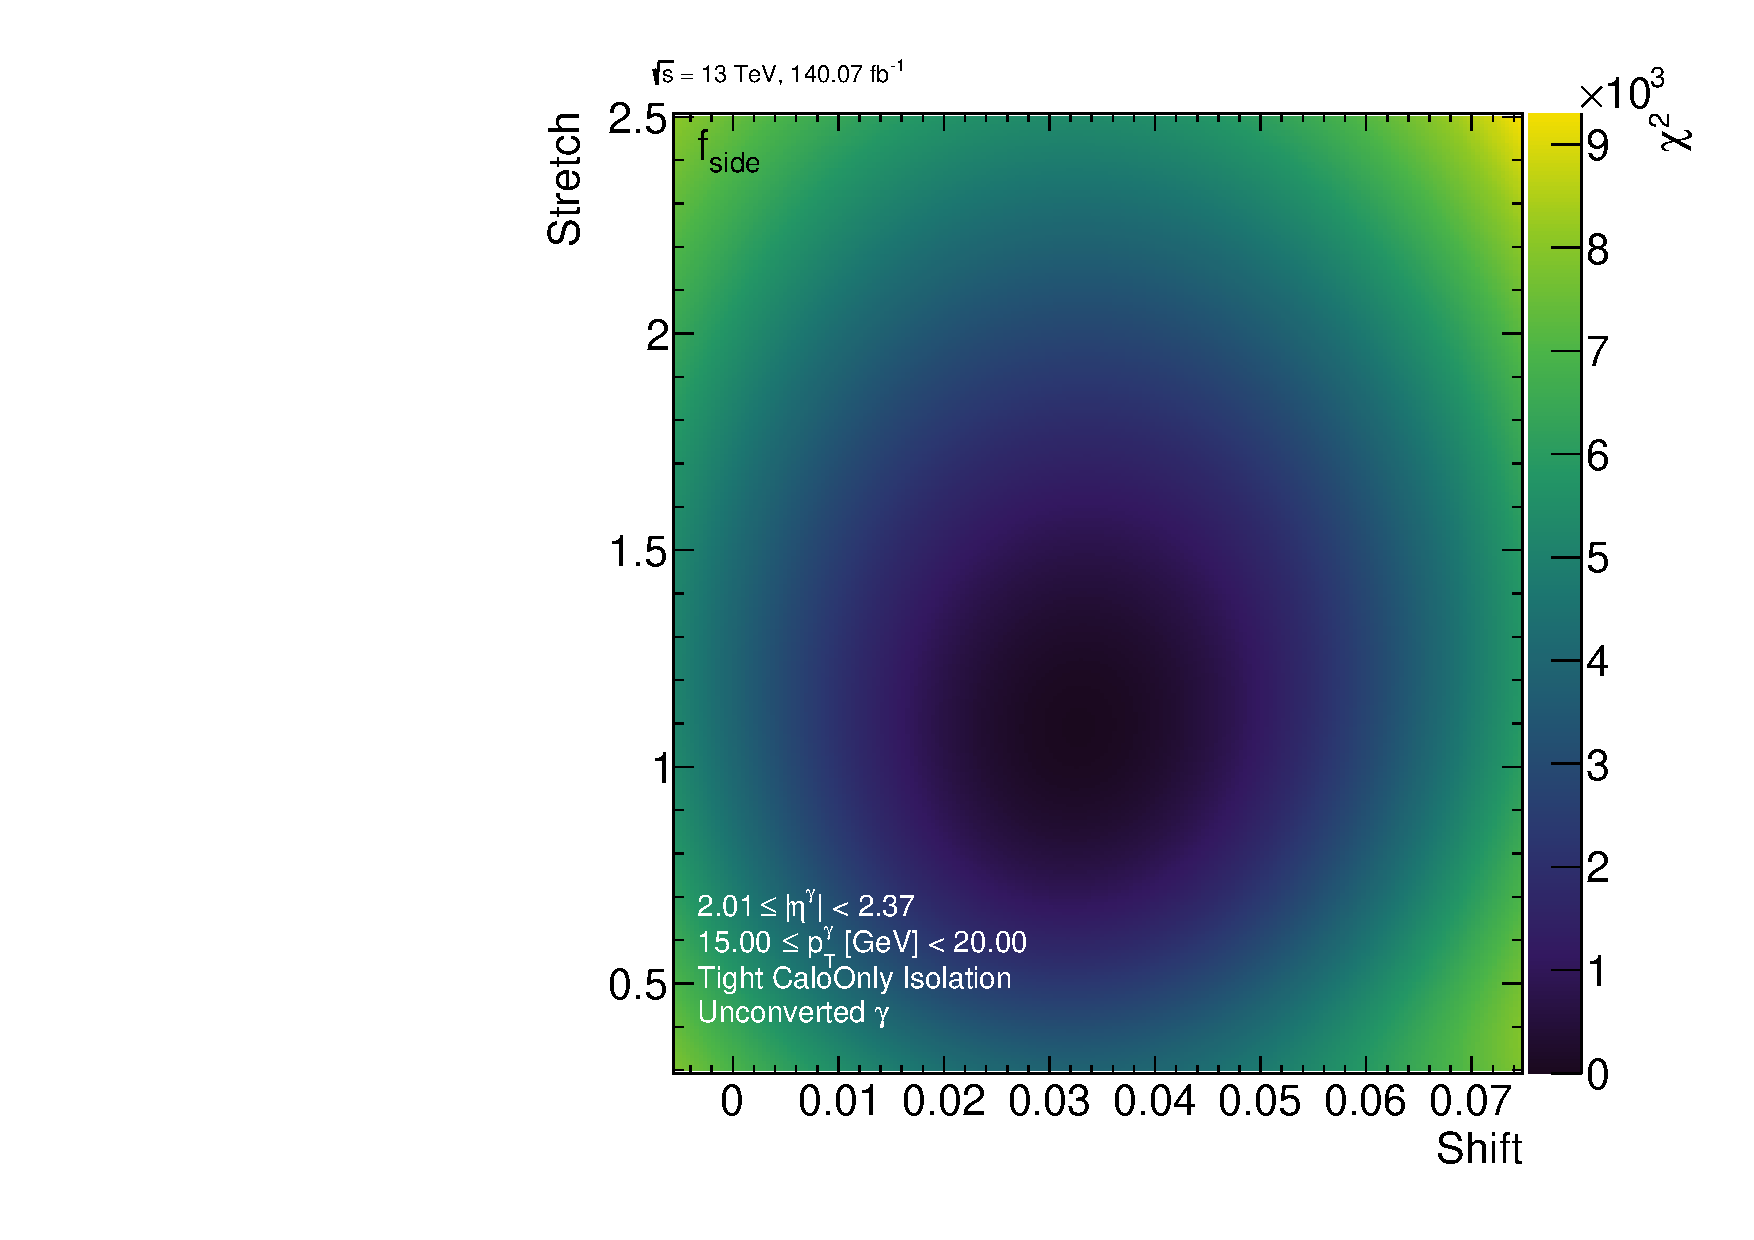
\includegraphics[width=\linewidth]{4_photonid/ffs/procedure/can2d__chi2scan_nocontour__ph_fside__Isotightcaloonly_IdNone_u_pt15p0_eta2p01}
        \caption{\chisq values in the shift-stretch plane.}
        \label{fig:ss_corrections:ffs:calculation:fside_calculation:chi2}
    \end{subfigure}
    \hfill
    \begin{subfigure}[t]{0.49\linewidth}
        \centering
        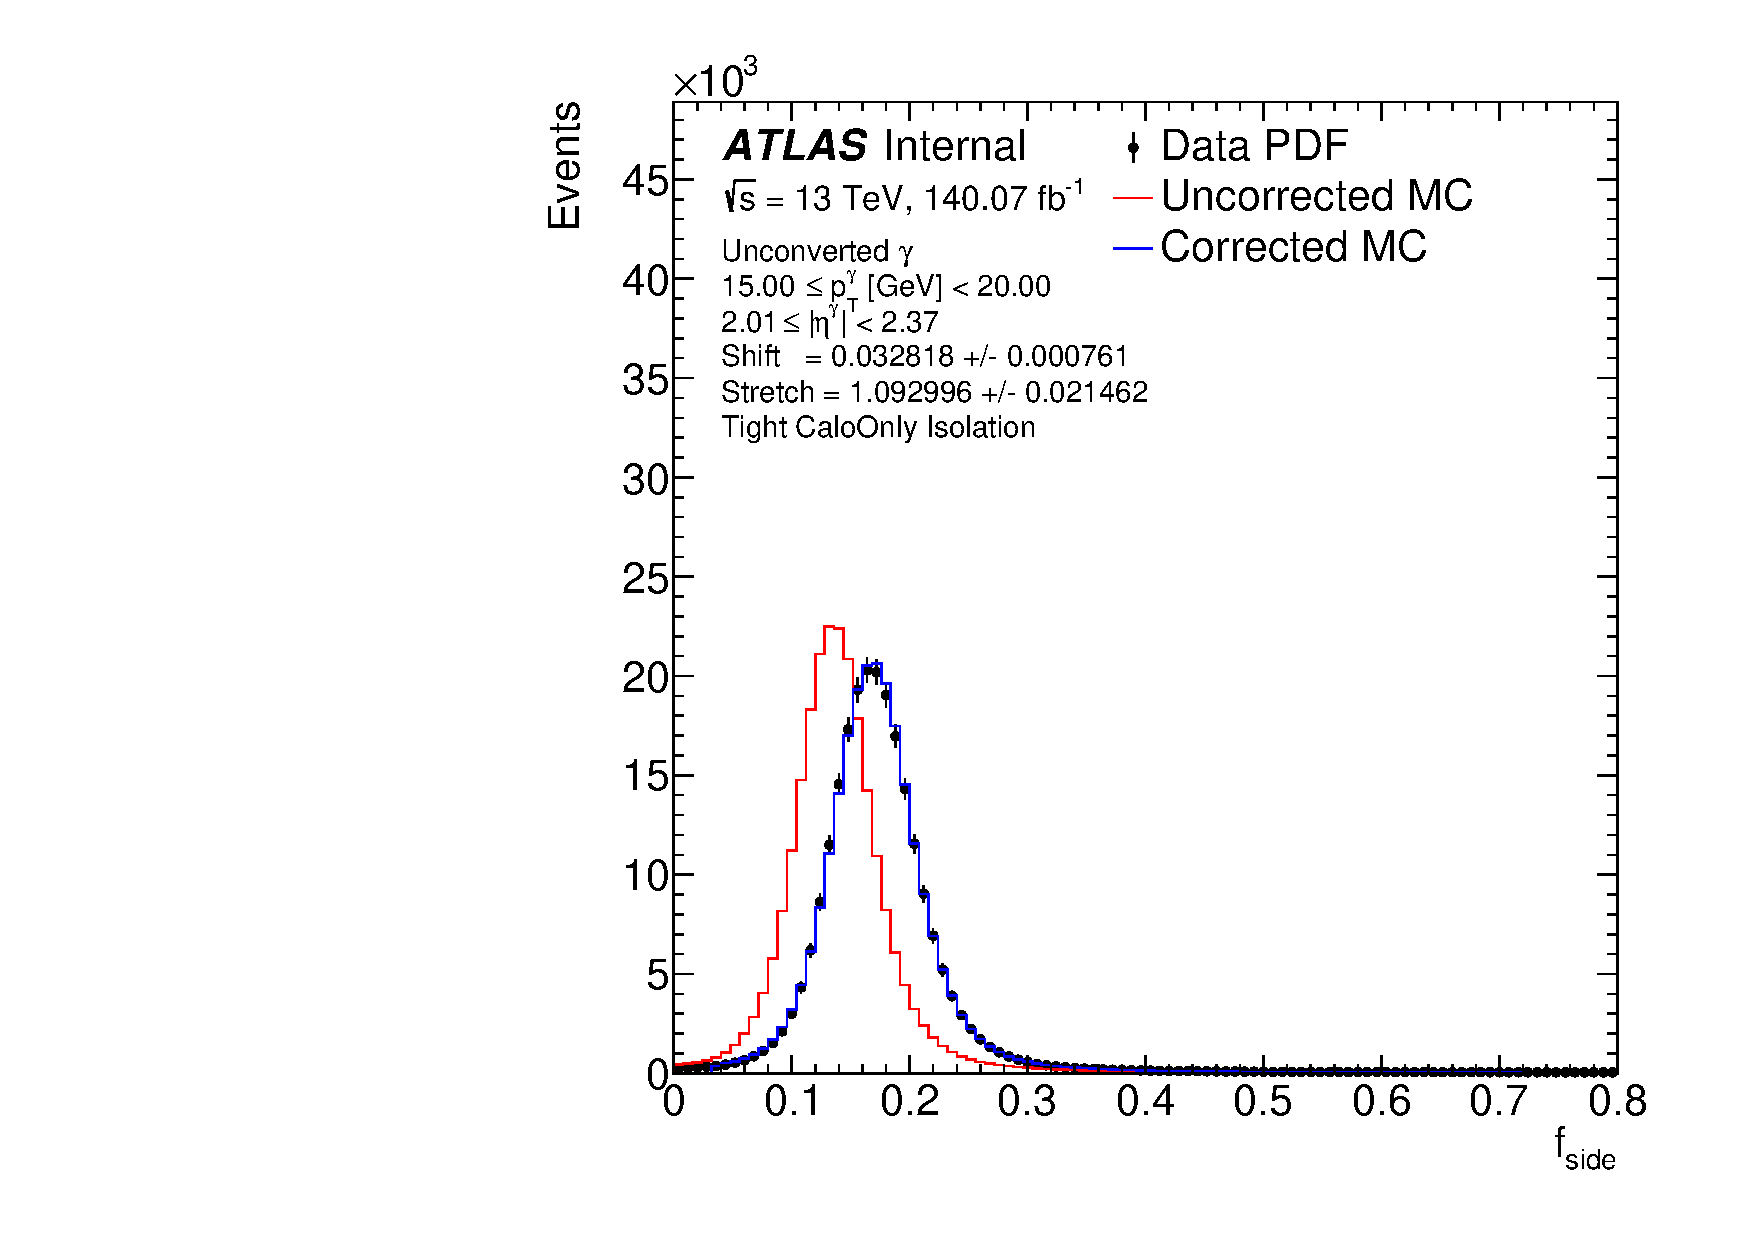
\includegraphics[width=\linewidth]{4_photonid/ffs/procedure/can__data_mc_fudged_comp__ph_fside__Isotightcaloonly_IdNone_u_pt15p0_eta2p01}
        \caption{Data (black points), uncorrected (red line) and corrected (blue line) \acp{PDF2} for the \fside variable, showing the impact of the \acp{FF}.}
        \label{fig:ss_corrections:ffs:calculation:fside_calculation:pdfs}
    \end{subfigure}
    \caption{Calculation of shift+stretch \acp{FF} for \fside with unconverted photons.}
    \label{fig:ss_corrections:ffs:calculation:fside_calculation}
\end{figure}







\subsection{Uncertainties}
\label{subsec:ss_corrections:ffs:uncs}

\subsubsection{Statistical uncertainties}

To extract the statistical uncertainties on the shift and stretch \acp{FF}, a fit to the \(1\sigma\) (\(68.3\%\) confidence level) contour on the \chisq values is performed. This contour represents an ellipse in the large sample limit which takes the following form:
\begin{equation}
    \chi^2 = \chi^2_{\text{min}} + \frac{1}{1-\rho^2} \left[ \left( \frac{x-x_0}{\sigma_x} \right)^2 + \left( \frac{y-y_0}{\sigma_y} \right)^2 - 2\rho \left( \frac{x-x_0}{\sigma_x} \right) \left( \frac{y-y_0}{\sigma_y} \right) \right],
\end{equation}
where \(\rho\) is the correlation coefficient between both variables, \(\sigma_x\) and \(\sigma_y\) the uncertainties on \(x\) and \(y\), respectively, \((x_0, y_0)\) is the location of the ellipse's center, and \(\chi^2_{\text{min}}\) is the \(\chi^2\) minimum value obtained from the 2D histogram.


By extracting the semi-major and semi-minor axes of the fitted ellipse, and with the tilt angle of it, the statistical uncertainties on two variables \(x\) and \(y\) (in this case representing the shift and stretch, respectively) are (see \App{\ref{app:ellipse_formulae}}):
\begin{gather}
    \sigma_x = \sqrt{a^2 \cos^2\theta + b^2 \sin^2\theta}\\
    \sigma_y = \sqrt{a^2 \sin^2\theta + b^2 \cos^2\theta}.
\end{gather}

\subsubsection{Systematic uncertainties}

The systematic uncertainties are derived by varying the preselection criteria, that is, photon identification and photon isolation. Changing different preselection criteria allows the \acp{SS} to vary depending on the amount of background contamination, and in consequence so do the \acp{FF}.
The different selections are:
\begin{itemize}
    \item \acf{RZ} sample:
        \begin{itemize}
            \item Nominal: No ID, \texttt{FixedCutTightCaloOnly} isolation.
            \item Loose ID, no isolation.
            \item Loose ID, \texttt{FixedCutTightCaloOnly} isolation.
            \item No ID, \texttt{FixedCutLoose} isolation.
        \end{itemize}
    \item \acf{SP} sample:
        \begin{itemize}
            \item Nominal: Tight ID, \texttt{FixedCutLoose} isolation.
            \item Tight ID, \texttt{FixedCutTight} isolation.
        \end{itemize}
\end{itemize}
All other combinations (or lack thereof) of selection criteria would result in either a sample with too low statistics, or too low purity.

\acp{FF} are derived for each one of the previous selections, and the difference between the nominal and the veried ones is calculated. The maximum difference is taken as the systematic uncertainty, as the most conservative approach.










\subsection{Results}
\label{subsec:ss_corrections:ffs:results}


Due to the fact that \acp{FF} are calculated in different \pt using two different samples which span complementary regions, the results are concatenated at \(50~\gev\). in the following, shift and stretch values are reported for different \ac{SS} variables.

The reported shift values in the figures are normalised by the standard deviation of the \ac{SS} after stretching, as this quantity allows to understand how much each variable is shifted with respect to its width. Also, it provides an unique measure for all considered variables, since they span different ranges. Nevertheless, the variables' width vary for different \pt-\abseta bins, leading to eventual large differences between neighbouring bins. In such cases, there are no drastic differences differences on the original shift values.

In \Fig{\ref{fig:ss_corrections:ffs:reslts:ffs}}, examples of resulting \acp{FF} for the \reta and \weta variables using converted photons are presented. It can be seen that for both variables the \acp{FF} depend on \pt, specially towards higher momenta and converted photons. This behaviour is also repeated on all variables.
By inspecting the behaviours and trends of the \acp{FF}, it is also possible to retrieve information on the \ac{MC} mismodelling of the \acp{SS}. As said in \Sect{\ref{sec:pid_ss:ss_differences}}, broader \(\eta\) widths and profiles were observed for data compared to the simulation. This is, in fact, still observed to present day, since the stretch values increase towards higher \pt, stretching the \ac{MC} simulations as much as twice theirs initial width. In the case of \reta (\weta) (for the displayed \abseta bin and converted photons), the \ac{MC} simulation overestimated (underestimated) the central value by almost a standard deviation after fixing the width, meanining that huge differences are still present in the uncorrected \ac{MC} distribution. 

\begin{figure}[ht!]
    \centering
    \begin{subfigure}[h]{0.49\linewidth}
        \centering
        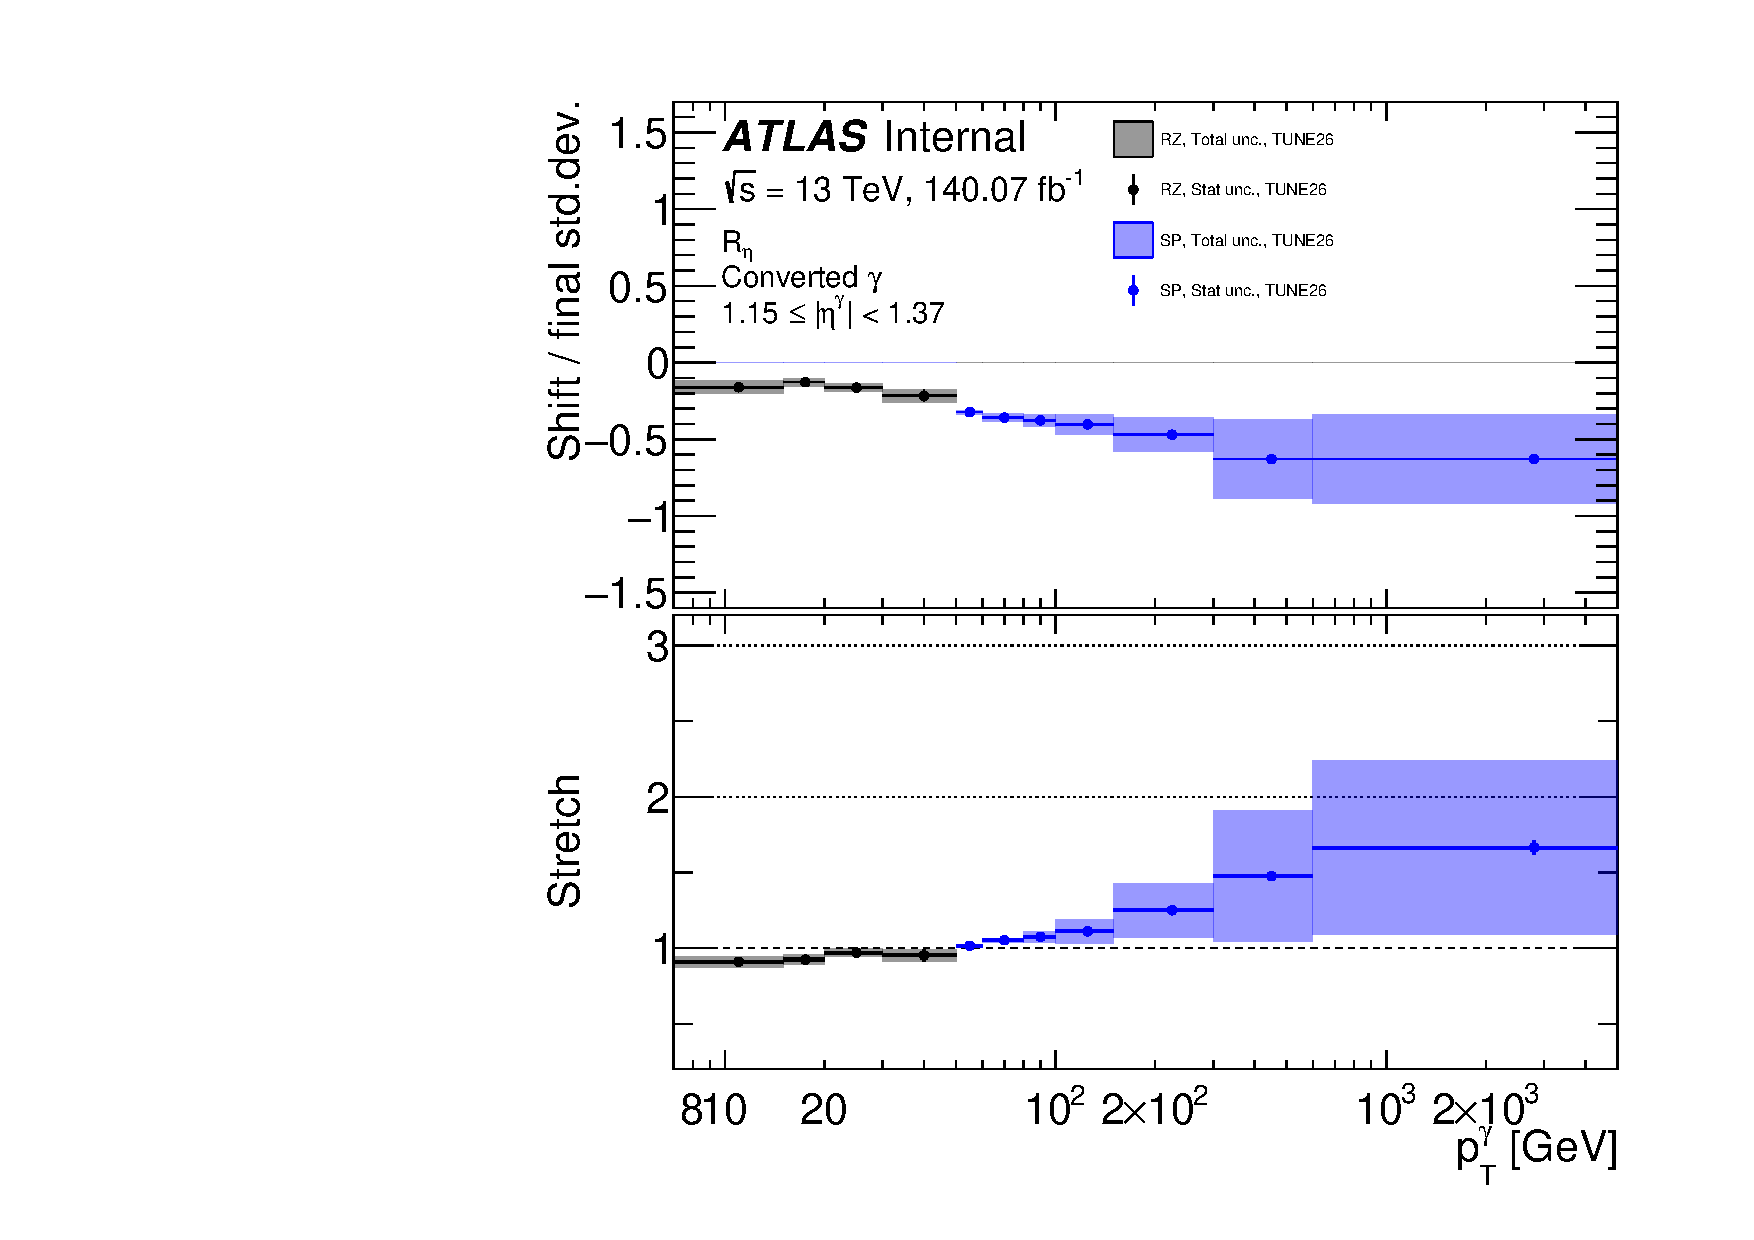
\includegraphics[width=\linewidth]{4_photonid/ffs/results/combined/1d/can__comb__ph_reta__c__eta1p15__shift_normalized}
        \caption{\reta}
        \label{fig:ss_corrections:ffs:reslts:ffs:reta}
    \end{subfigure}
    \hfill
    \begin{subfigure}[h]{0.49\linewidth}
        \centering
        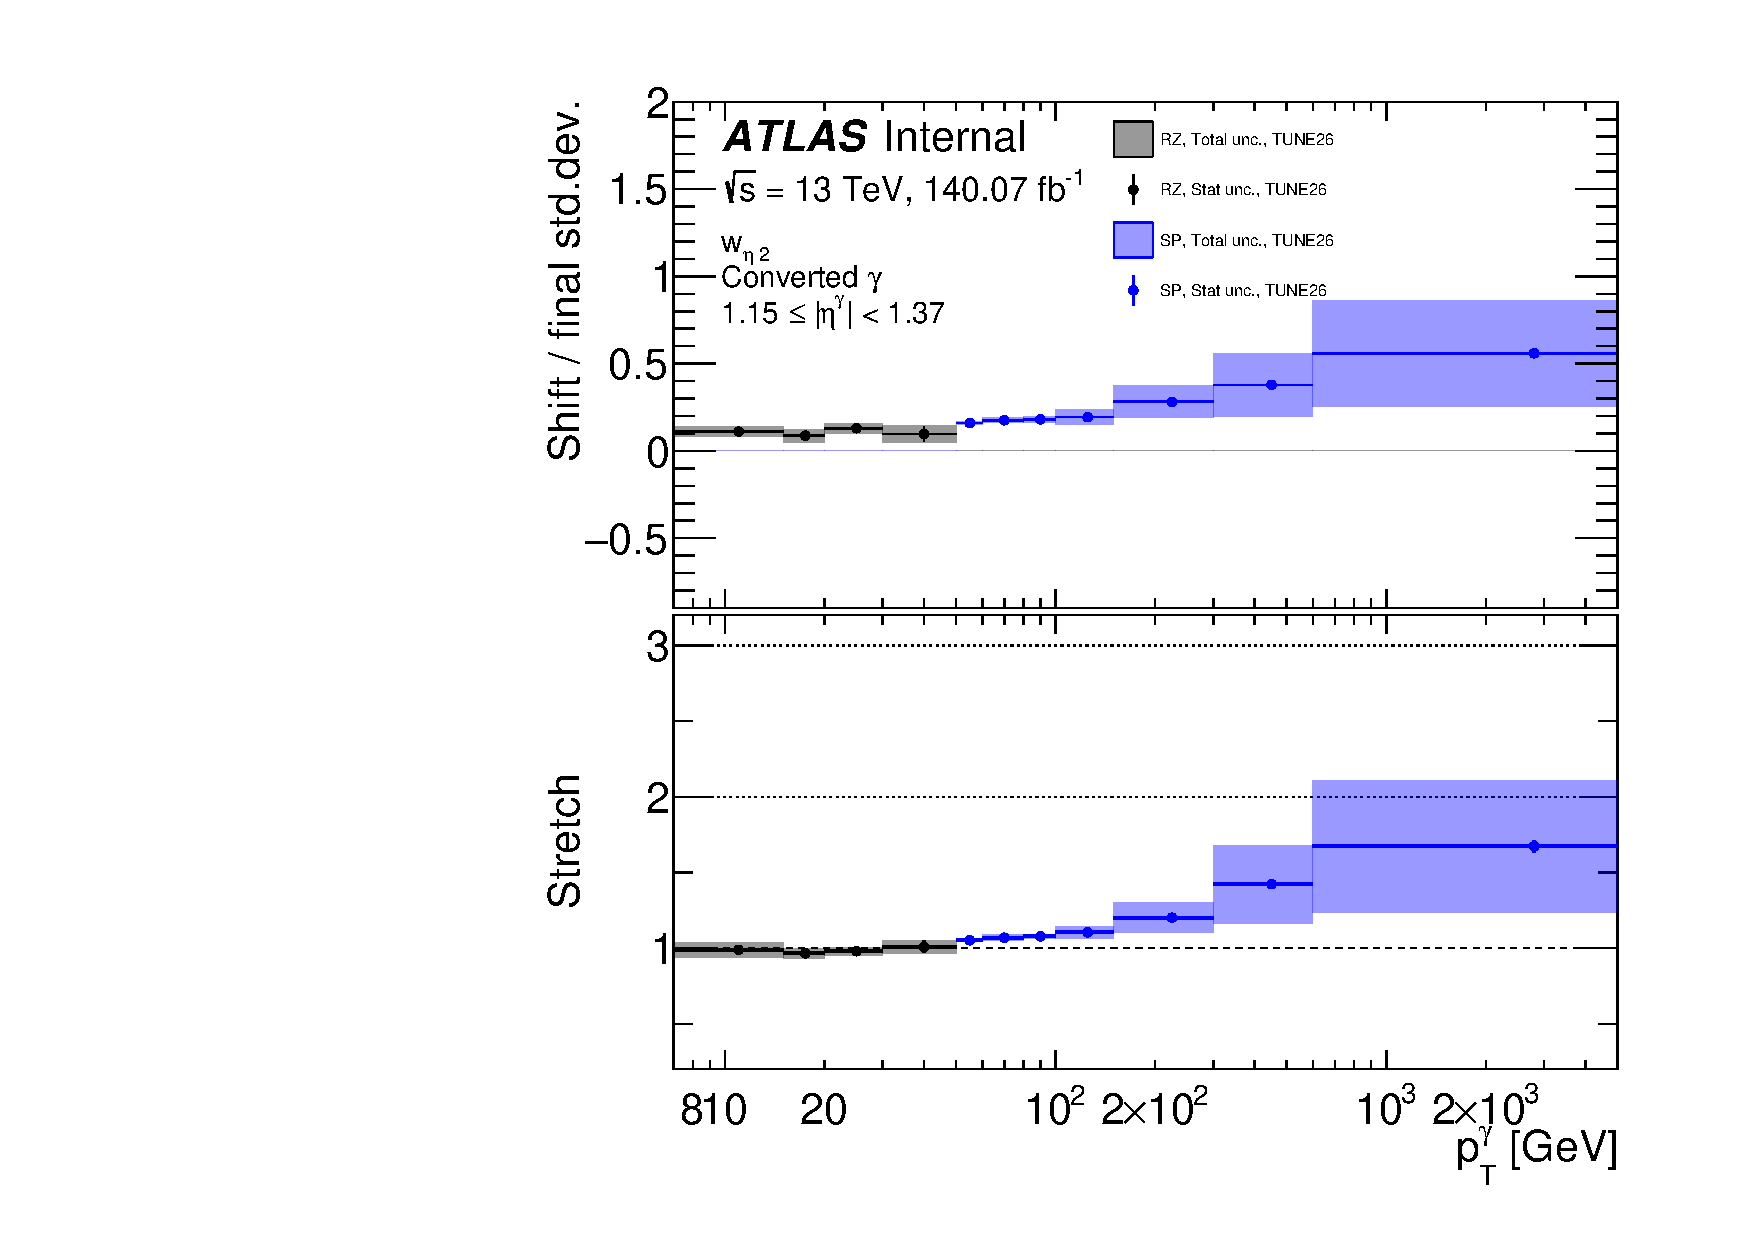
\includegraphics[width=\linewidth]{4_photonid/ffs/results/combined/1d/can__comb__ph_weta2__c__eta1p15__shift_normalized}
        \caption{\weta}
        \label{fig:ss_corrections:ffs:reslts:ffs:weta}
    \end{subfigure}
    \caption{Shift and stretch \acp{FF} for \reta (left) and \weta (right) \acp{SS} for converted photons as a function of the photon \pt with \(1.15<\abseta<1.37\). Results from \ac{RZ} (black) and \ac{SP} (blue) are displayed, where the shaded regions denote the total uncertainty, while the error bars only the statistical one. Stretch values are shown in the bottom pad. The shift, on the other hand, is shown in the top pad, which are normalised by the standard deviation of the \ac{SS} after applying the stretch, as indicated in the text.}
    \label{fig:ss_corrections:ffs:reslts:ffs}
\end{figure}

It is also useful to visualise the \acp{FF} for a fixed \pt-bin and as a function of \abseta. This is shown for \wstot using converted photons with \(50<\pt<60~\gev\) in \Fig{\ref{fig:ss_corrections:ffs:reslts:ffs_eta_wstot}} where the normalised and raw shift values are displayed. For \(\abseta>1.81\) (last two bins), normalised shift values are greater than previous bins by, at least, a factor of 2. However, the raw shift values shown in \Fig{\ref{fig:ss_corrections:ffs:reslts:ffs_eta_wstot:raw_shift}} do not present such an abrupt change, indicating that this is a direct consequence of the change of width of the distributions.


\begin{figure}[ht!]
    \centering
    \begin{subfigure}[h]{0.49\linewidth}
        \centering
        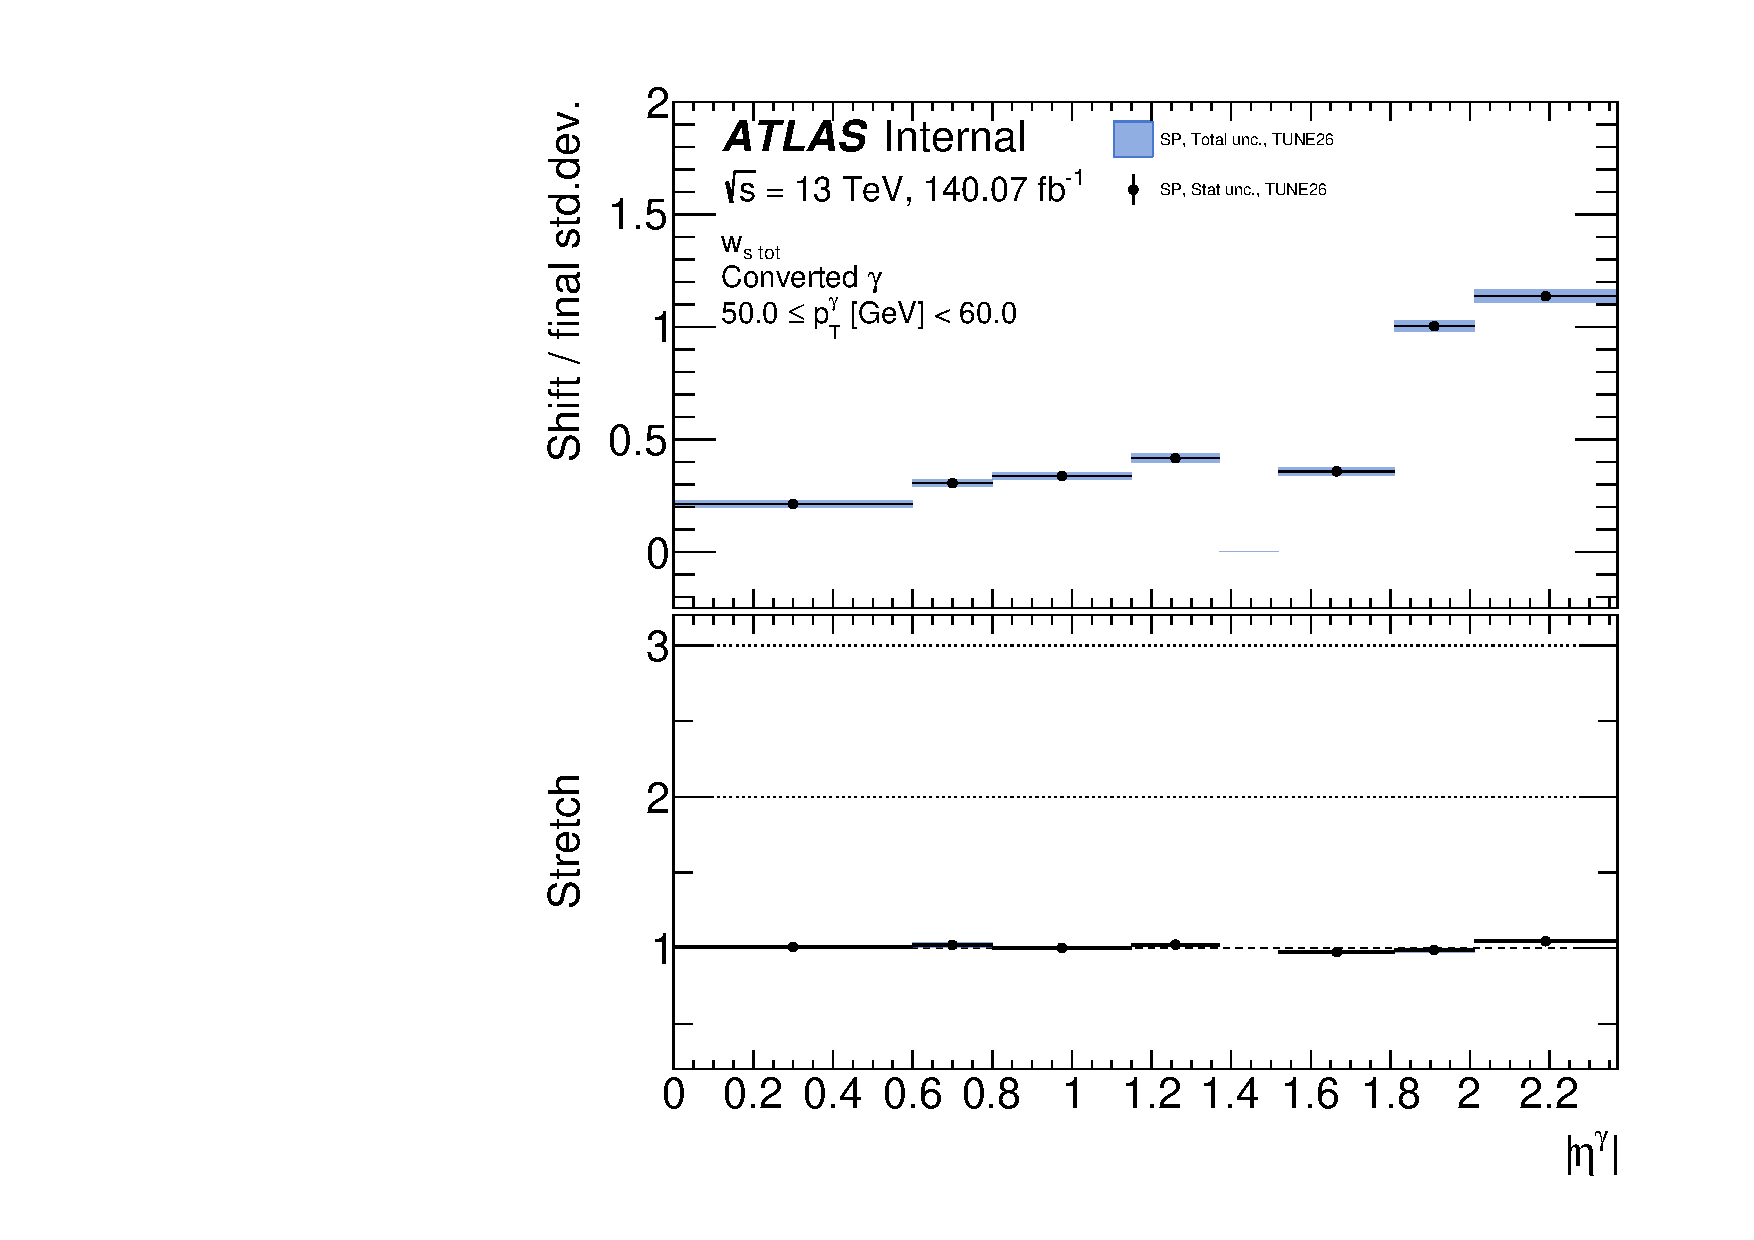
\includegraphics[width=\linewidth]{4_photonid/ffs/results/SP/1d/can__SP__ph_wstot__c__pt0050p0__shift_normalized}
        \caption{Normalised shift values.}
        \label{fig:ss_corrections:ffs:reslts:ffs_eta_wstot:normalised_shift}
    \end{subfigure}
    \hfill
    \begin{subfigure}[h]{0.49\linewidth}
        \centering
        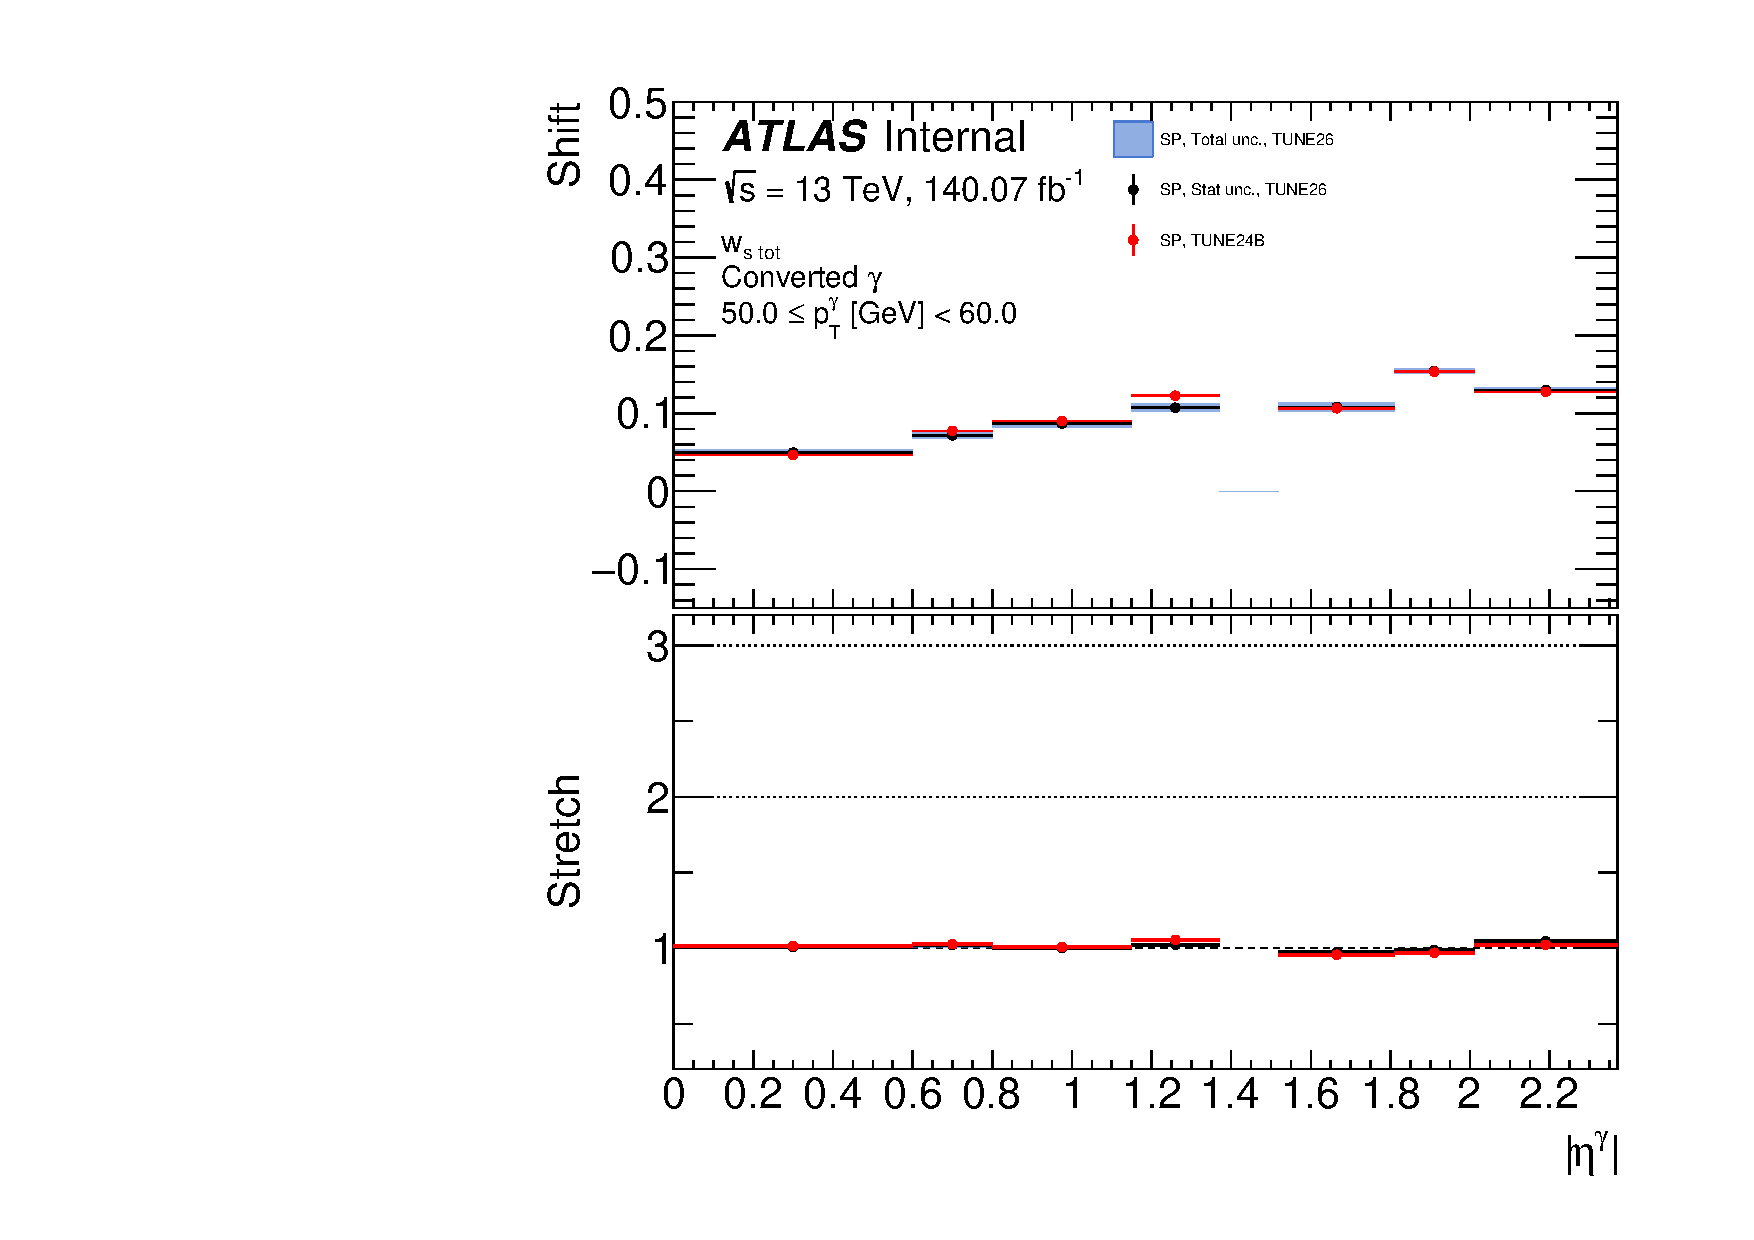
\includegraphics[width=\linewidth]{4_photonid/ffs/results/SP/1d/can__SP__ph_wstot__c__pt0050p0}
        \caption{Raw shift values.}
        \label{fig:ss_corrections:ffs:reslts:ffs_eta_wstot:raw_shift}
    \end{subfigure}\\
    \caption{Shift and stretch \acp{FF} for \wstot \acp{SS} using converted photons as a function of \abseta and photons from the \ac{SP} with \(50<\pt<60~\gev\). Normalised shift values are displayed in \Fig{\subref{fig:ss_corrections:ffs:reslts:ffs_eta_wstot:normalised_shift}} while original, or raw, values are shown in \Fig{\subref{fig:ss_corrections:ffs:reslts:ffs_eta_wstot:raw_shift}}. Points with the uncertainty bar show the statistical uncertainty only, and the shaded regions represent the total uncertainty. Stretch values are shown in the bottom pad. Shift values are displayed in the top pad, which are normalised by the standard deviation of the \ac{SS} after applying the stretch.}
    \label{fig:ss_corrections:ffs:reslts:ffs_eta_wstot}
\end{figure}


In order to validate the obtained \acp{FF}, the corrections are applied to the \acp{SS} event-by-event.
\Figs{\ref{fig:ss_corrections:ffs:results:ss_rz}}{\ref{fig:ss_corrections:ffs:results:ss_sp}} show the application of the \acp{FF} to some of the \ac{SS} distributions using the \ac{RZ} and \ac{SP} samples, respectively, divided into the barrel and endcap regions in \abseta. In the barrel region, the corrections indeed improve the agreement, but the magnitudes of these corrections are not as dramatic as in the endcap region, where huge improvements are seen. Taking the \wone and \wstot variables as an example, major shape differences are observed between the nominal simulation and data, which the shift+stretch methods manage to fix. The same behaviour is observed using the \ac{SP} samples, where these variables present two or more peaks, and they are correctly fixed by the \acp{FF}. In all the shown cases, the corrected \ac{MC} and data are almost undistinguishable showing the importance of these corrections and how they were improved.

\begin{figure}[ht!]
    \centering
    \begin{subfigure}[h]{0.32\linewidth}
        \centering
        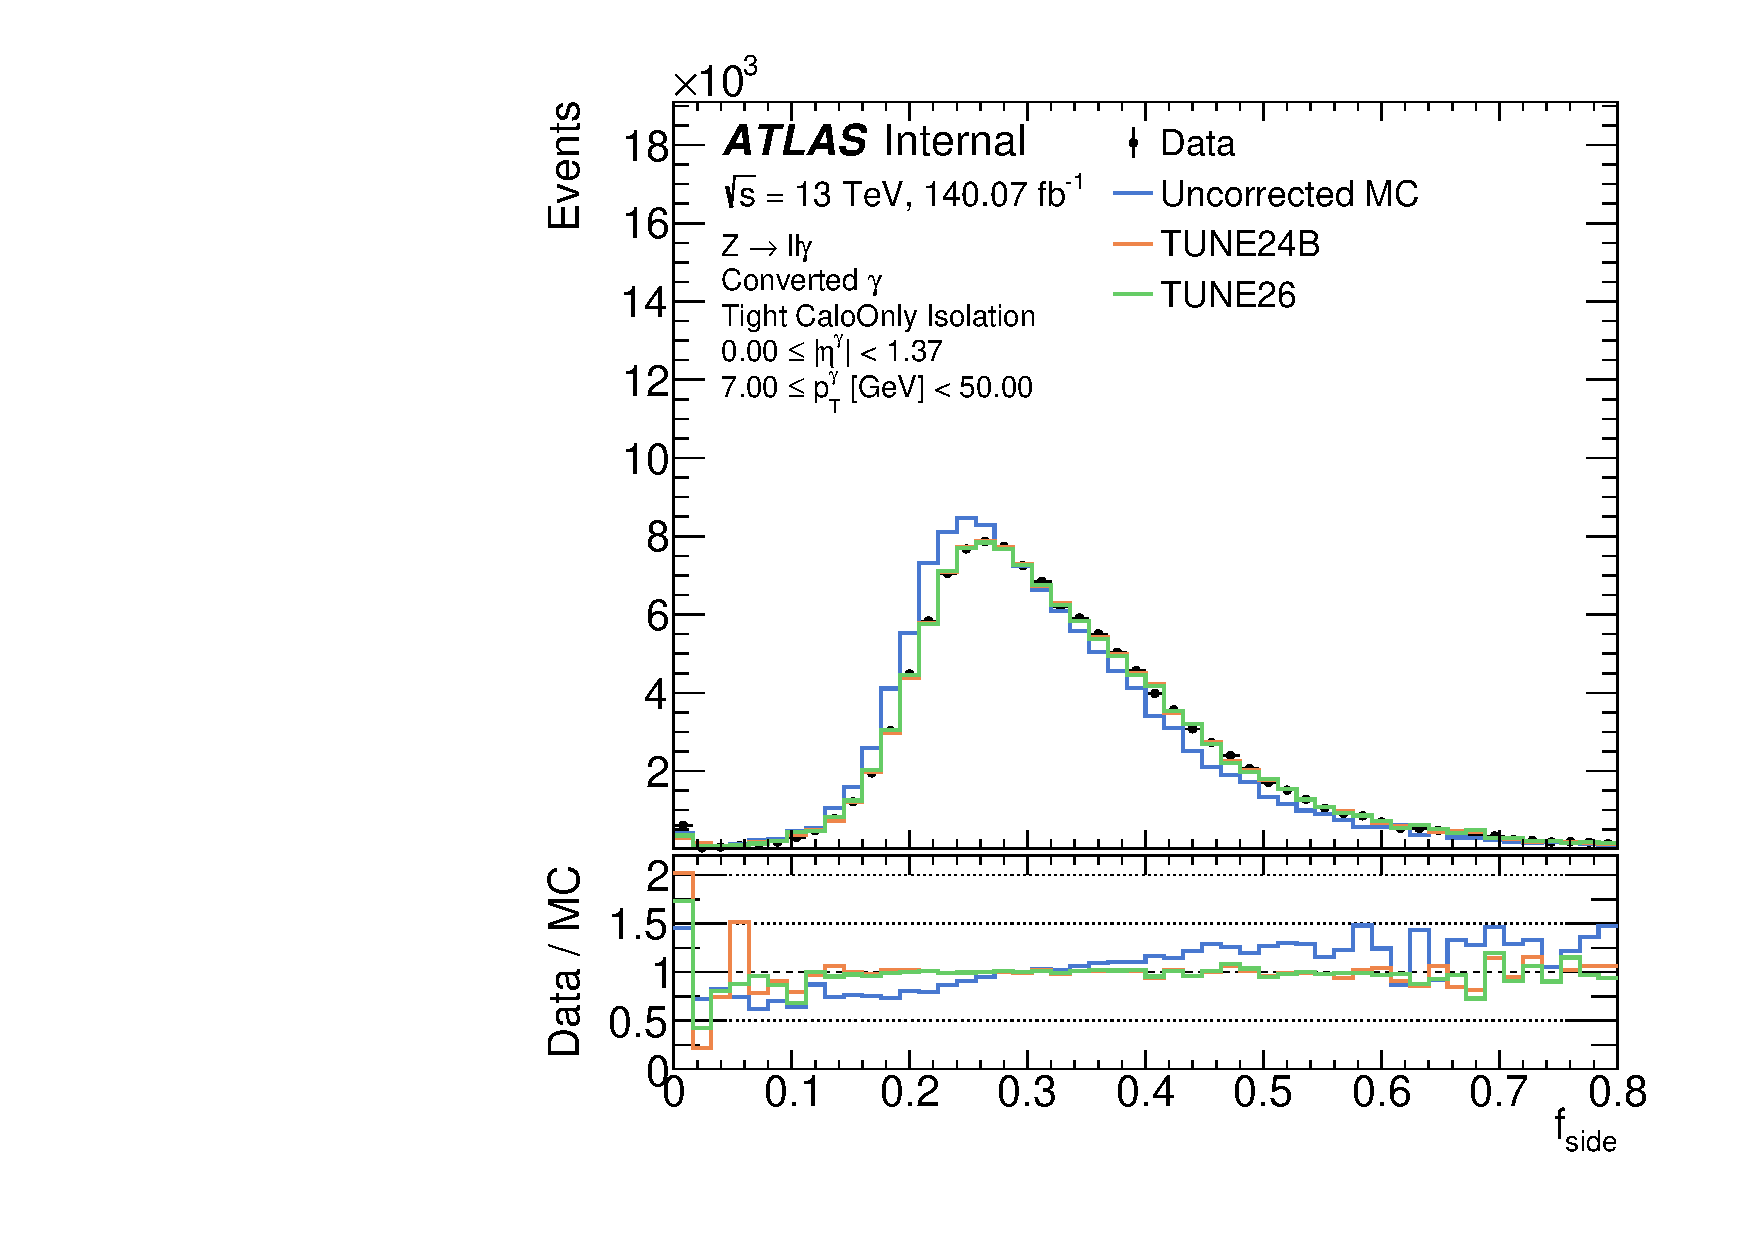
\includegraphics[width=\linewidth]{4_photonid/ffs/results/RZ/corrections/c/ptFull/etaCoarse/can__correction__ph_fside__Isotightcaloonly_IdNone__c__ptFullpt07p0__etaCoarseeta0p00}
        \caption{\fside, barrel.}
    \end{subfigure}
    \hfill
    \begin{subfigure}[h]{0.32\linewidth}
        \centering
        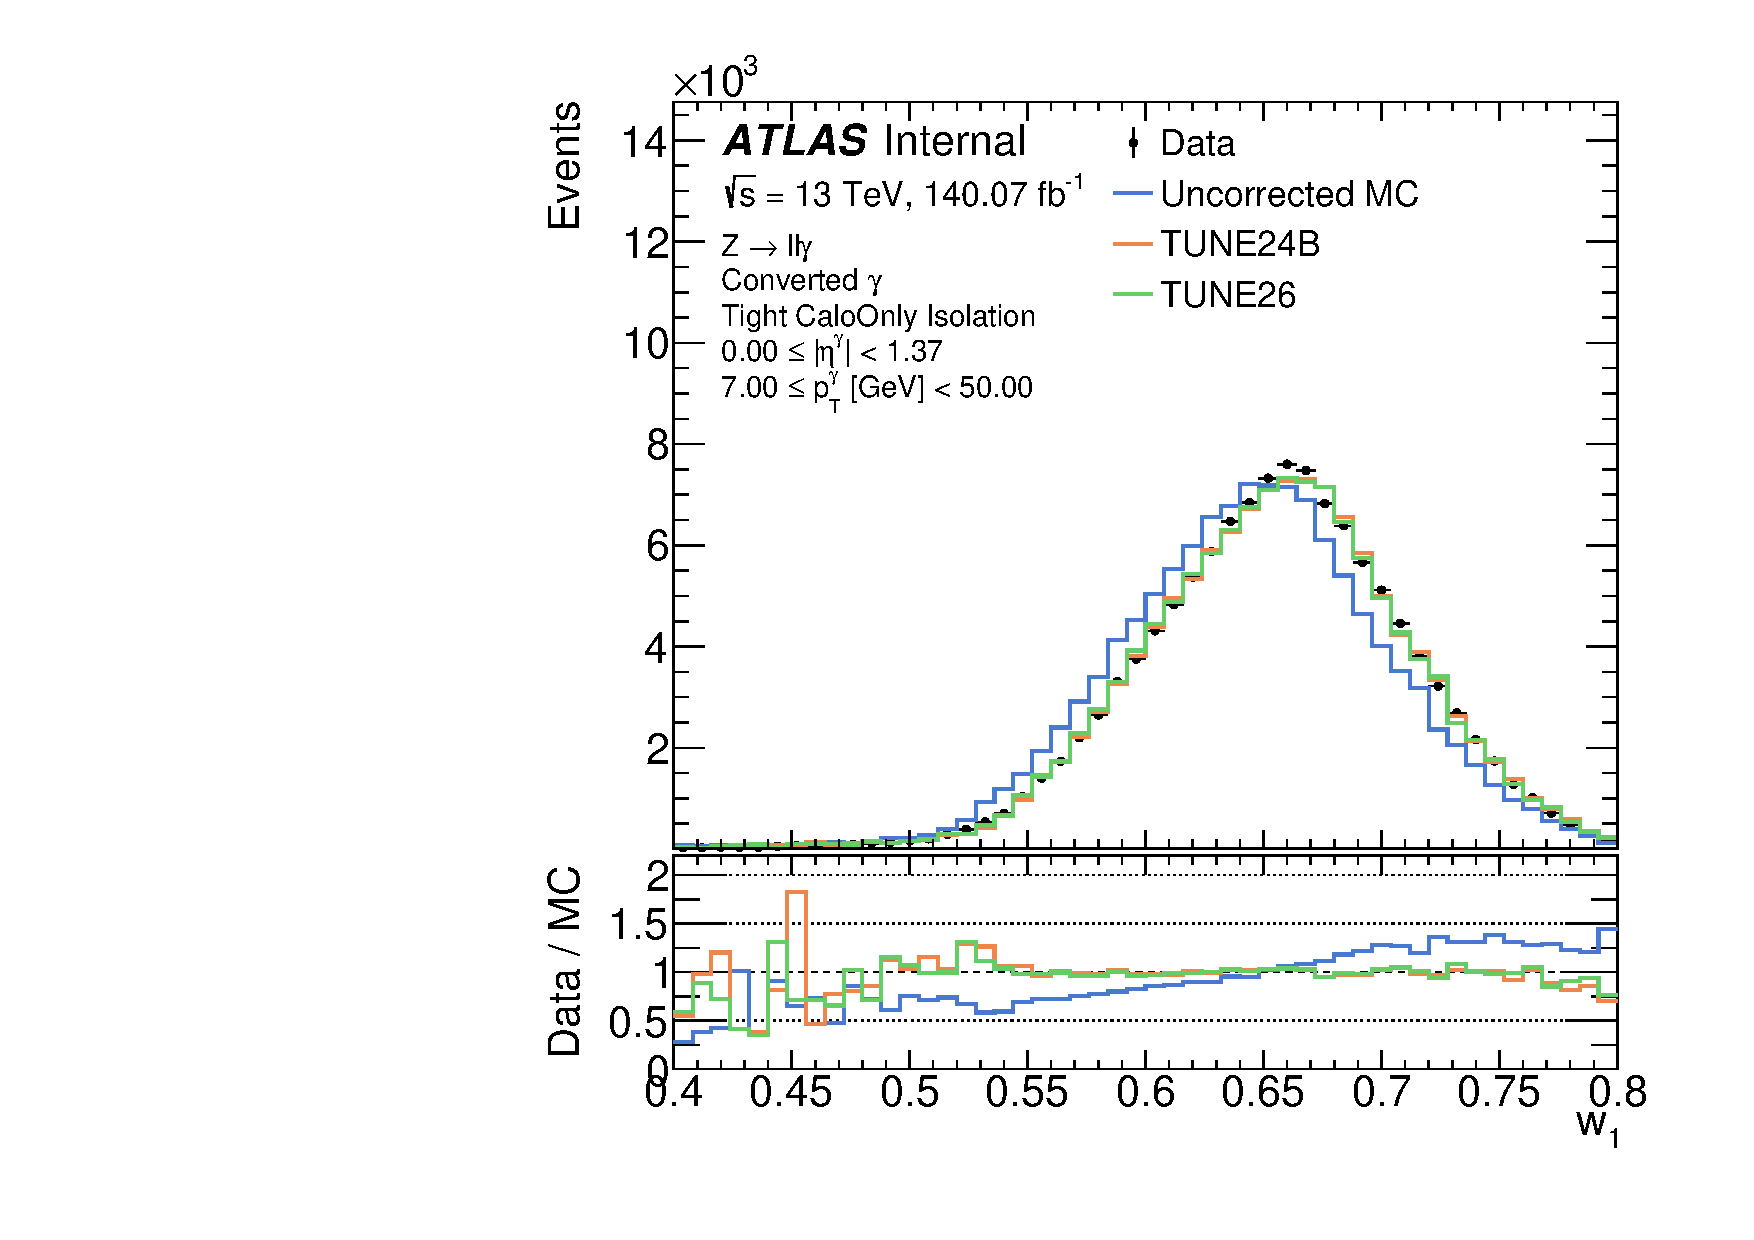
\includegraphics[width=\linewidth]{4_photonid/ffs/results/RZ/corrections/c/ptFull/etaCoarse/can__correction__ph_w1__Isotightcaloonly_IdNone__c__ptFullpt07p0__etaCoarseeta0p00}
        \caption{\wone, barrel.}
    \end{subfigure}
    \hfill
    \begin{subfigure}[h]{0.32\linewidth}
        \centering
        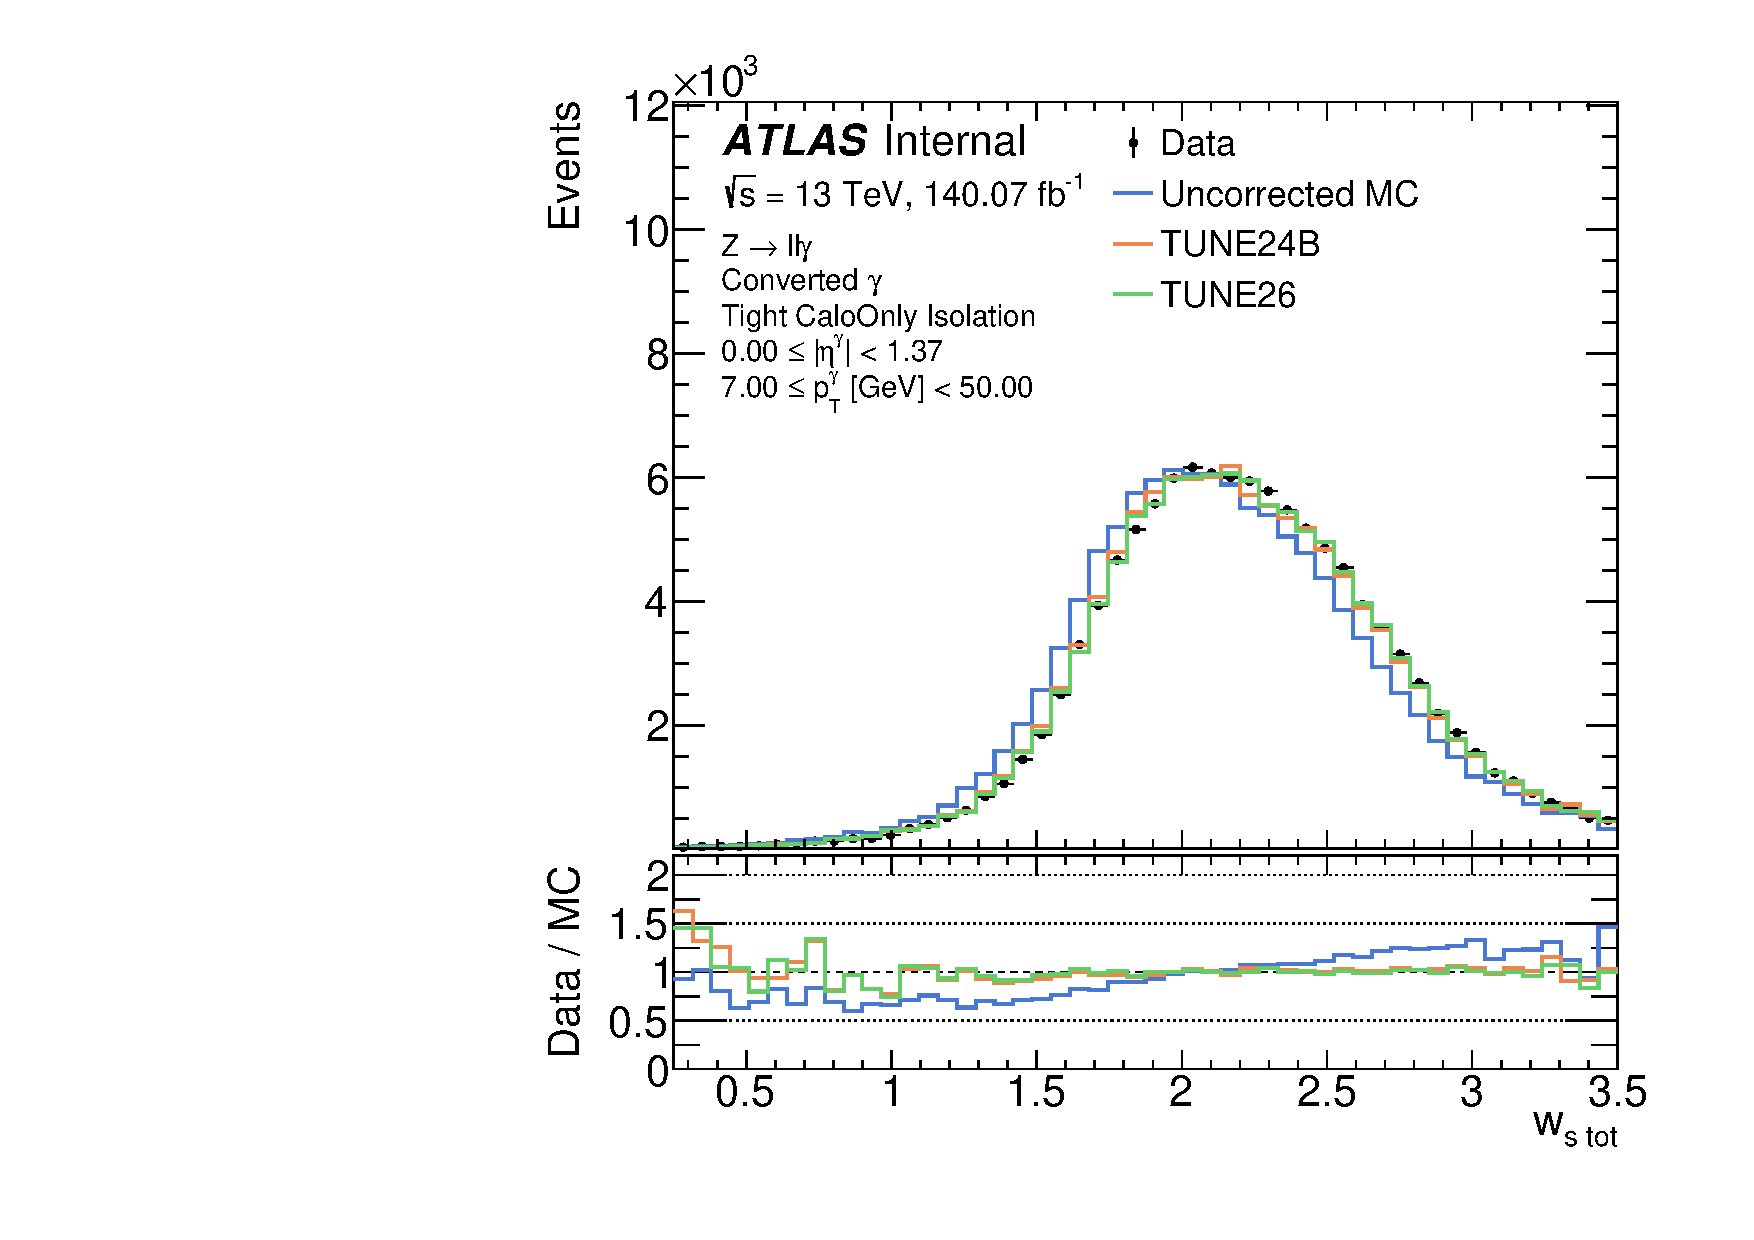
\includegraphics[width=\linewidth]{4_photonid/ffs/results/RZ/corrections/c/ptFull/etaCoarse/can__correction__ph_wstot__Isotightcaloonly_IdNone__c__ptFullpt07p0__etaCoarseeta0p00}
        \caption{\wstot, barrel.}
    \end{subfigure}\\
    \begin{subfigure}[h]{0.32\linewidth}
        \centering
        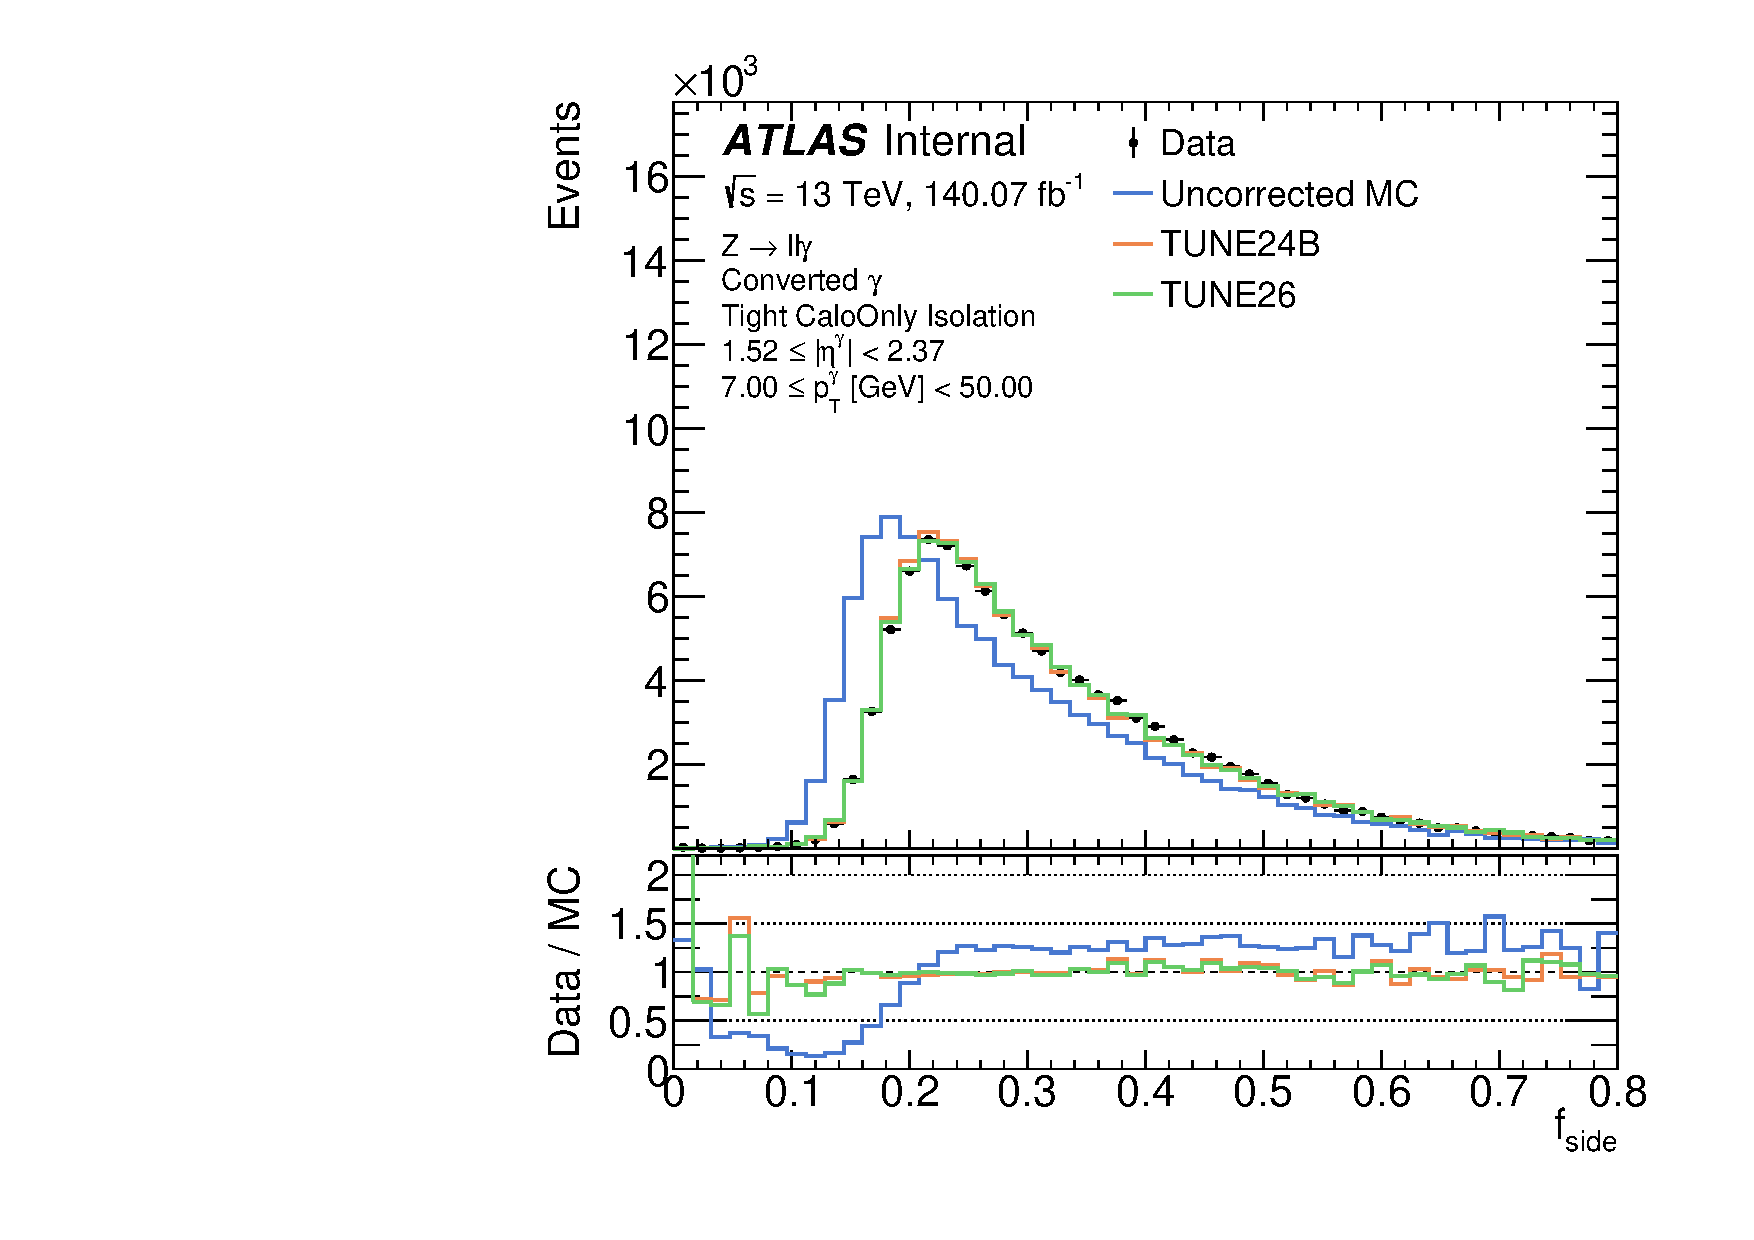
\includegraphics[width=\linewidth]{4_photonid/ffs/results/RZ/corrections/c/ptFull/etaCoarse/can__correction__ph_fside__Isotightcaloonly_IdNone__c__ptFullpt07p0__etaCoarseeta1p52}
        \caption{\fside, endcap.}
    \end{subfigure}
    \hfill
    \begin{subfigure}[h]{0.32\linewidth}
        \centering
        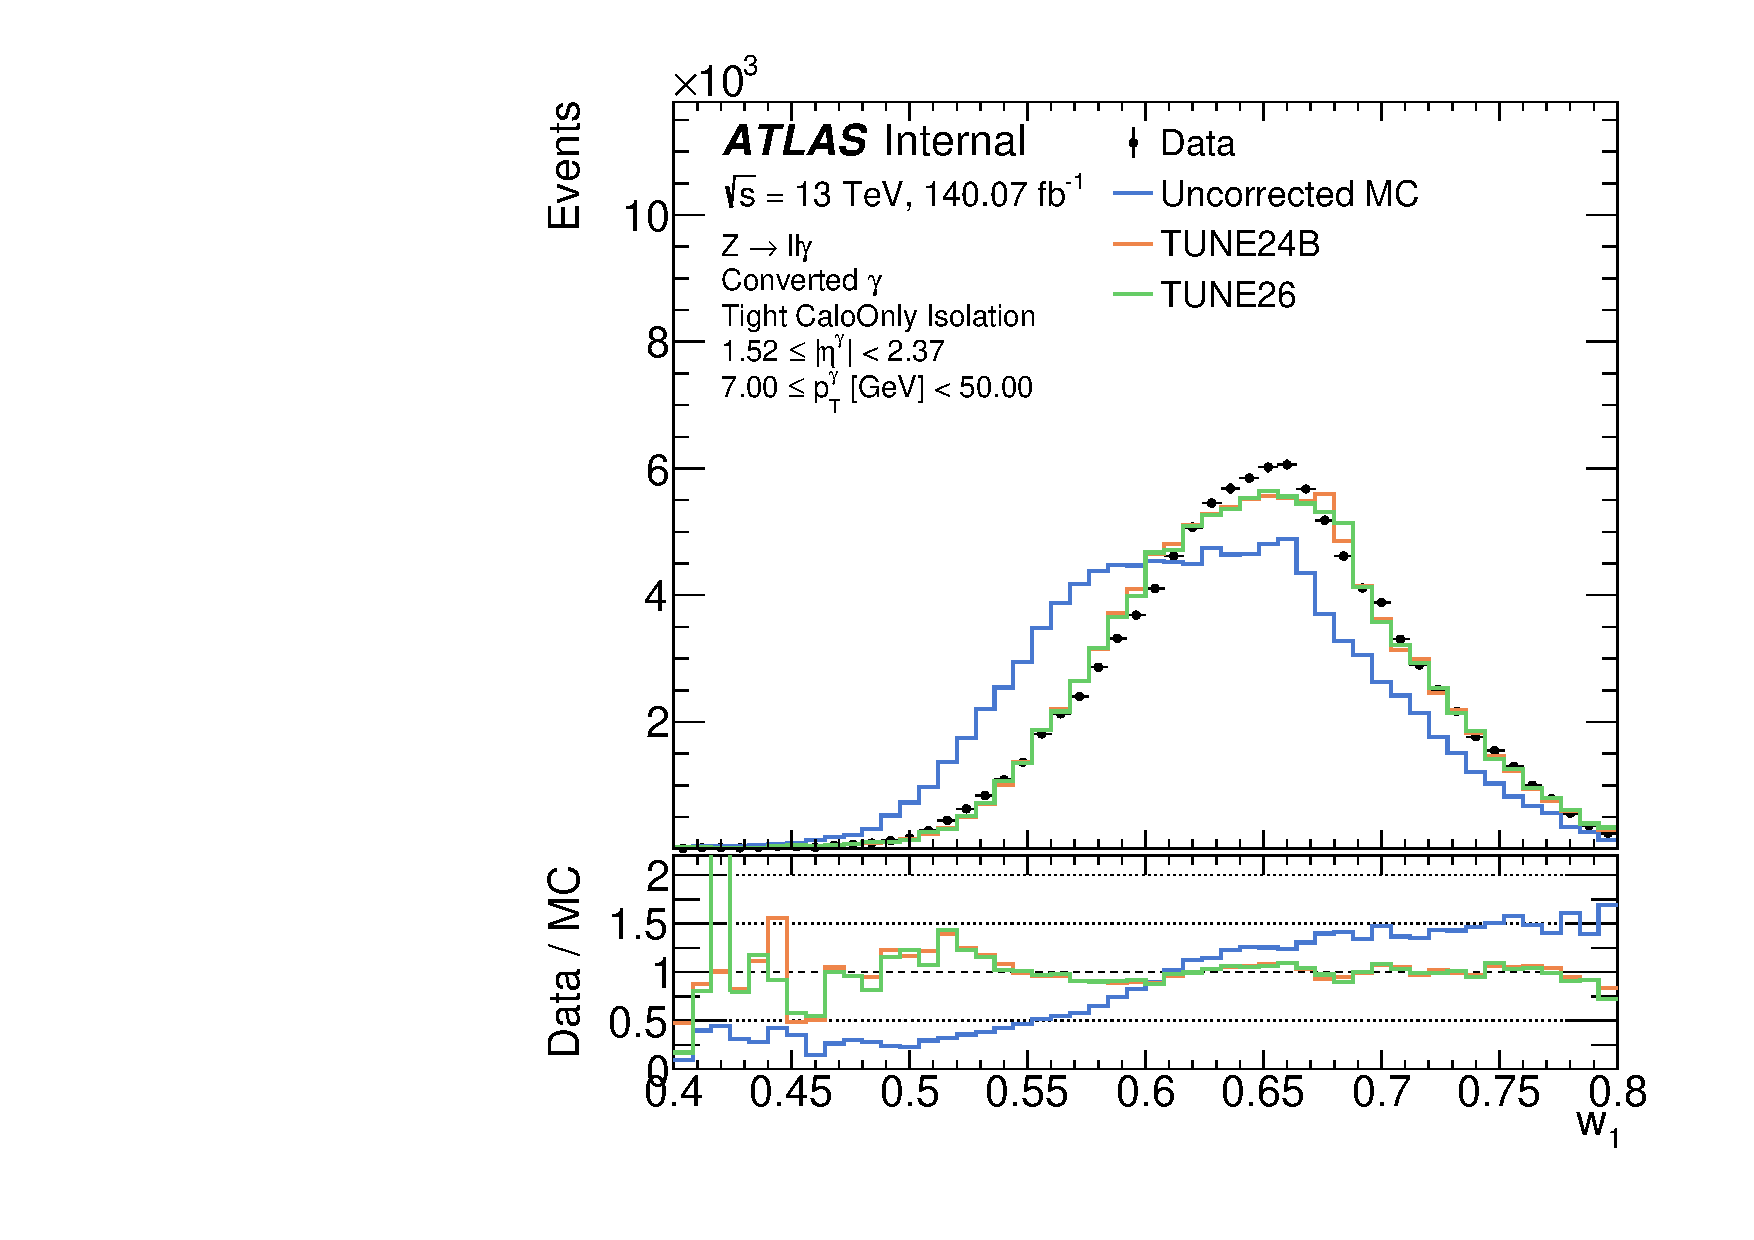
\includegraphics[width=\linewidth]{4_photonid/ffs/results/RZ/corrections/c/ptFull/etaCoarse/can__correction__ph_w1__Isotightcaloonly_IdNone__c__ptFullpt07p0__etaCoarseeta1p52}
        \caption{\wone, endcap.}
    \end{subfigure}
    \hfill
    \begin{subfigure}[h]{0.32\linewidth}
        \centering
        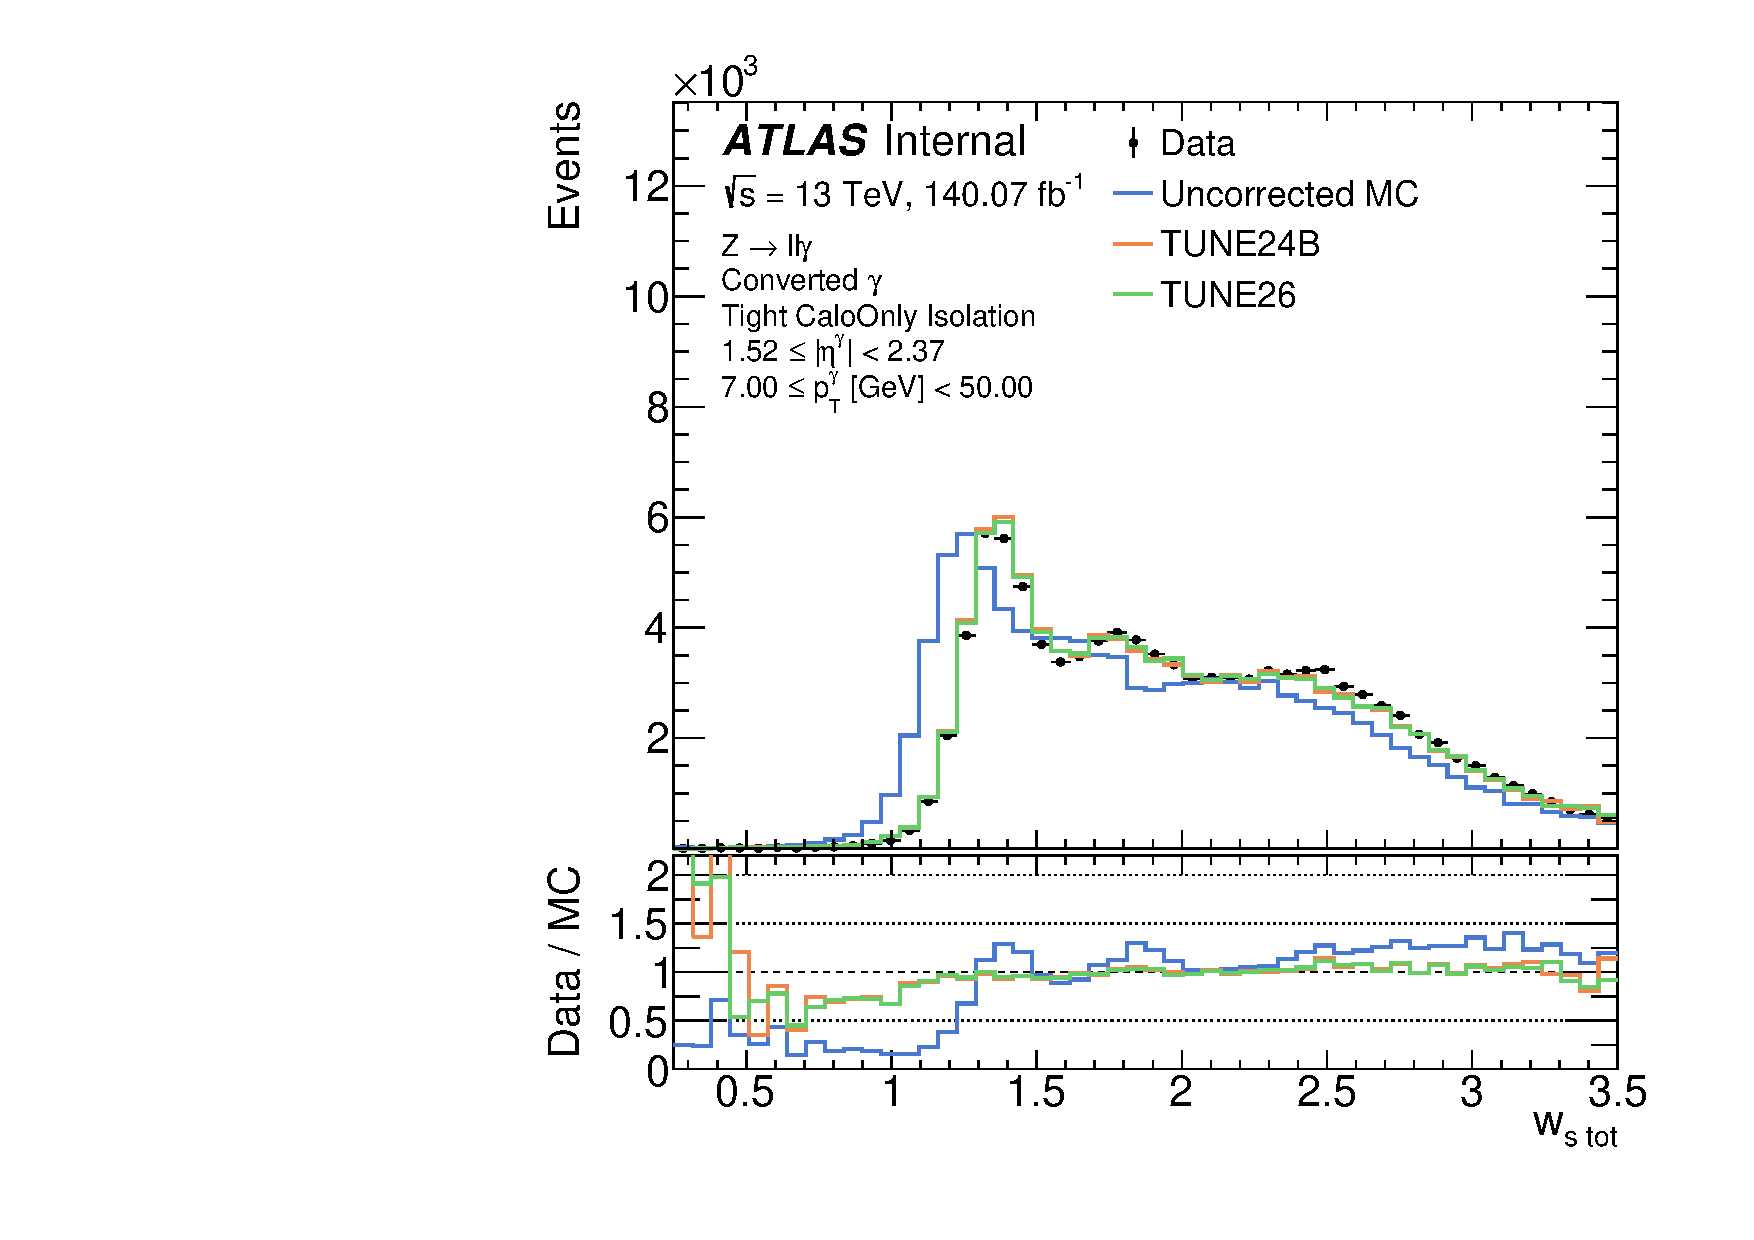
\includegraphics[width=\linewidth]{4_photonid/ffs/results/RZ/corrections/c/ptFull/etaCoarse/can__correction__ph_wstot__Isotightcaloonly_IdNone__c__ptFullpt07p0__etaCoarseeta1p52}
        \caption{\wstot, endcap.}
    \end{subfigure}\\
    \caption{Selected \acp{SS} distributions using the \ac{RZ} samples for converted photons after applying the \acp{FF} corrections event-by-event to the \ac{MC} simulation. The \acp{SS} are shown in the barrel region (top) and in the endcap (bottom). Data points are represented by the black points and uncorrected (corrected) \ac{MC} simulation by the blue (green) lines. The bottom pads show the ratio of data to the corresponding \ac{MC} simulation.}
    \label{fig:ss_corrections:ffs:results:ss_rz}
\end{figure}

\begin{figure}[ht!]
    \centering
    \begin{subfigure}[h]{0.32\linewidth}
        \centering
        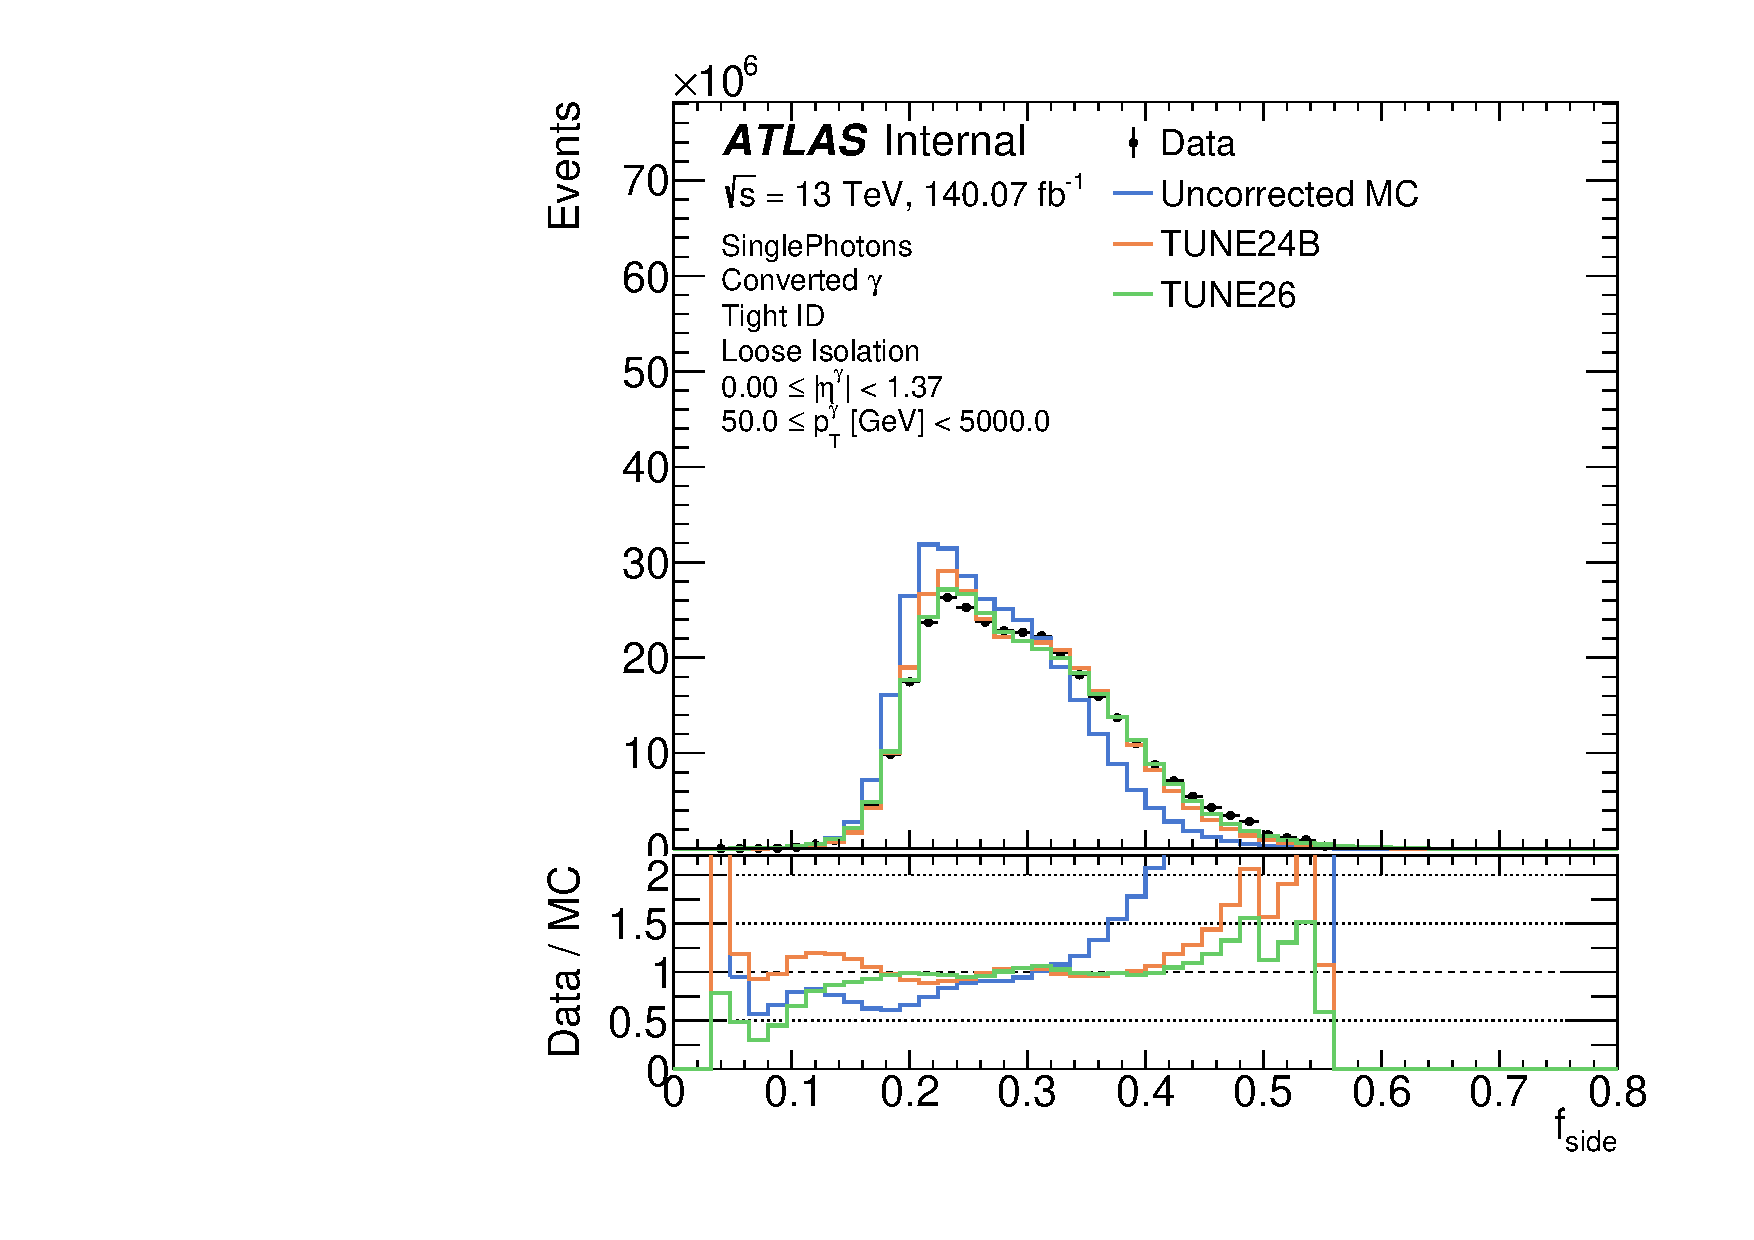
\includegraphics[width=\linewidth]{4_photonid/ffs/results/SP/corrections/c/ptFull/etaCoarse/can__correction__ph_fside__Isoloose_Idtight__c__ptFullpt0050p0__etaCoarseeta0p00}
        \caption{\fside, barrel.}
    \end{subfigure}
    \hfill
    \begin{subfigure}[h]{0.32\linewidth}
        \centering
        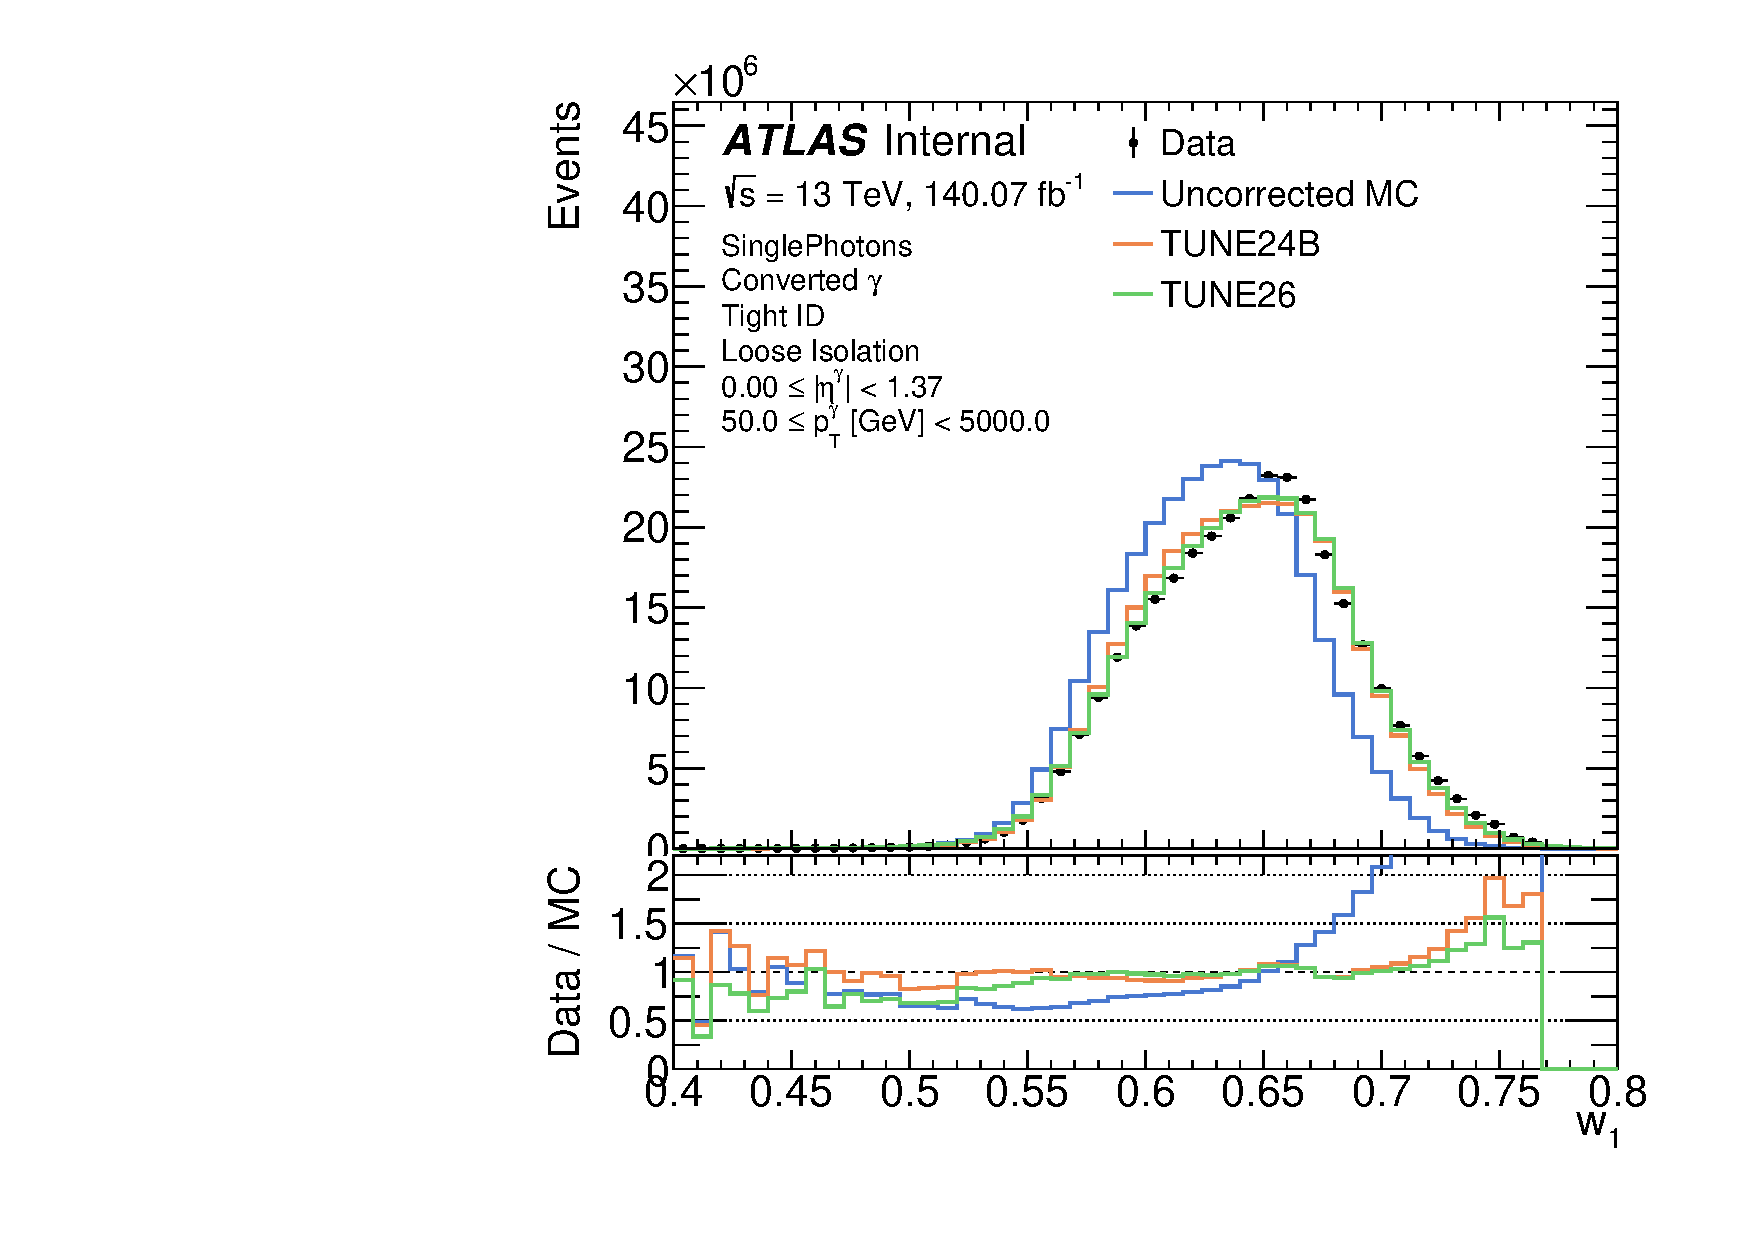
\includegraphics[width=\linewidth]{4_photonid/ffs/results/SP/corrections/c/ptFull/etaCoarse/can__correction__ph_w1__Isoloose_Idtight__c__ptFullpt0050p0__etaCoarseeta0p00}
        \caption{\wone, barrel.}
    \end{subfigure}
    \hfill
    \begin{subfigure}[h]{0.32\linewidth}
        \centering
        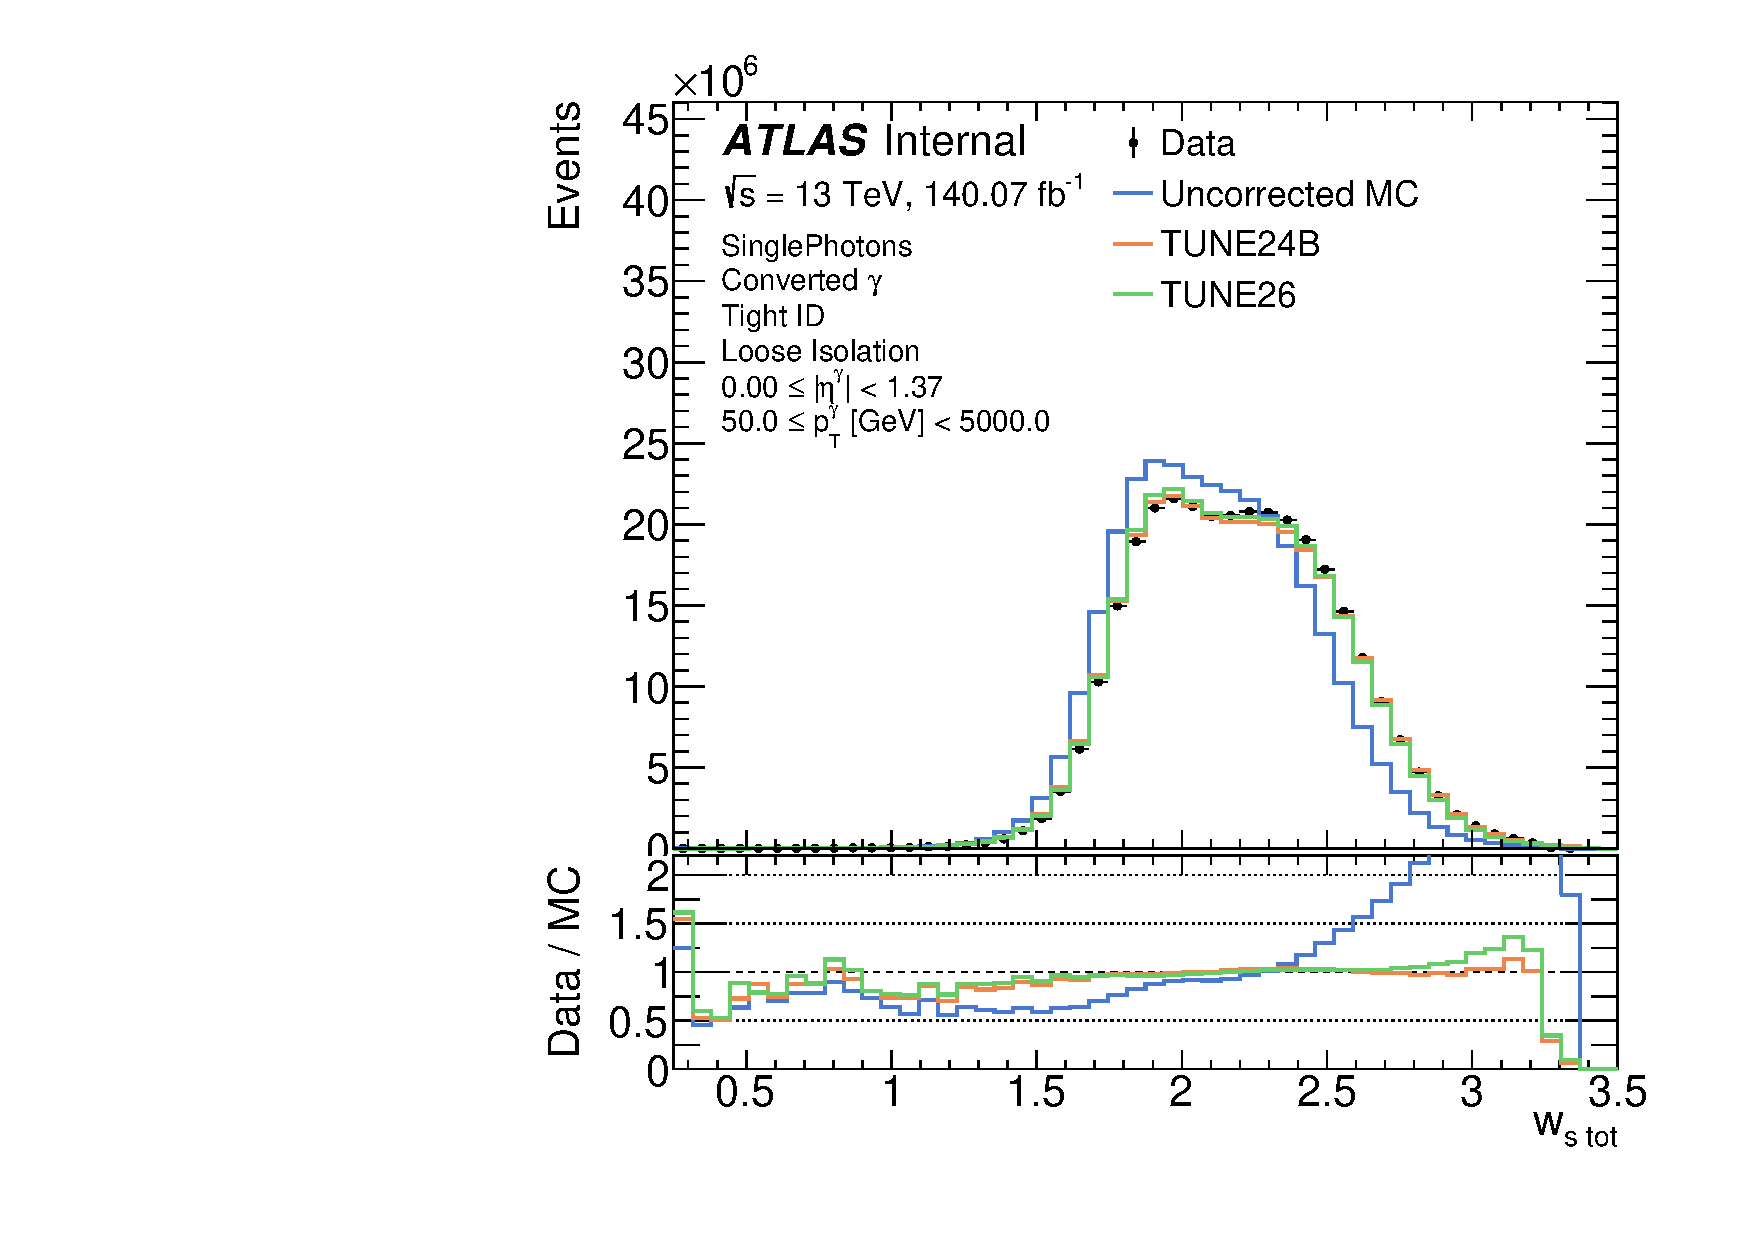
\includegraphics[width=\linewidth]{4_photonid/ffs/results/SP/corrections/c/ptFull/etaCoarse/can__correction__ph_wstot__Isoloose_Idtight__c__ptFullpt0050p0__etaCoarseeta0p00}
        \caption{\wstot, barrel.}
    \end{subfigure}\\
    \begin{subfigure}[h]{0.32\linewidth}
        \centering
        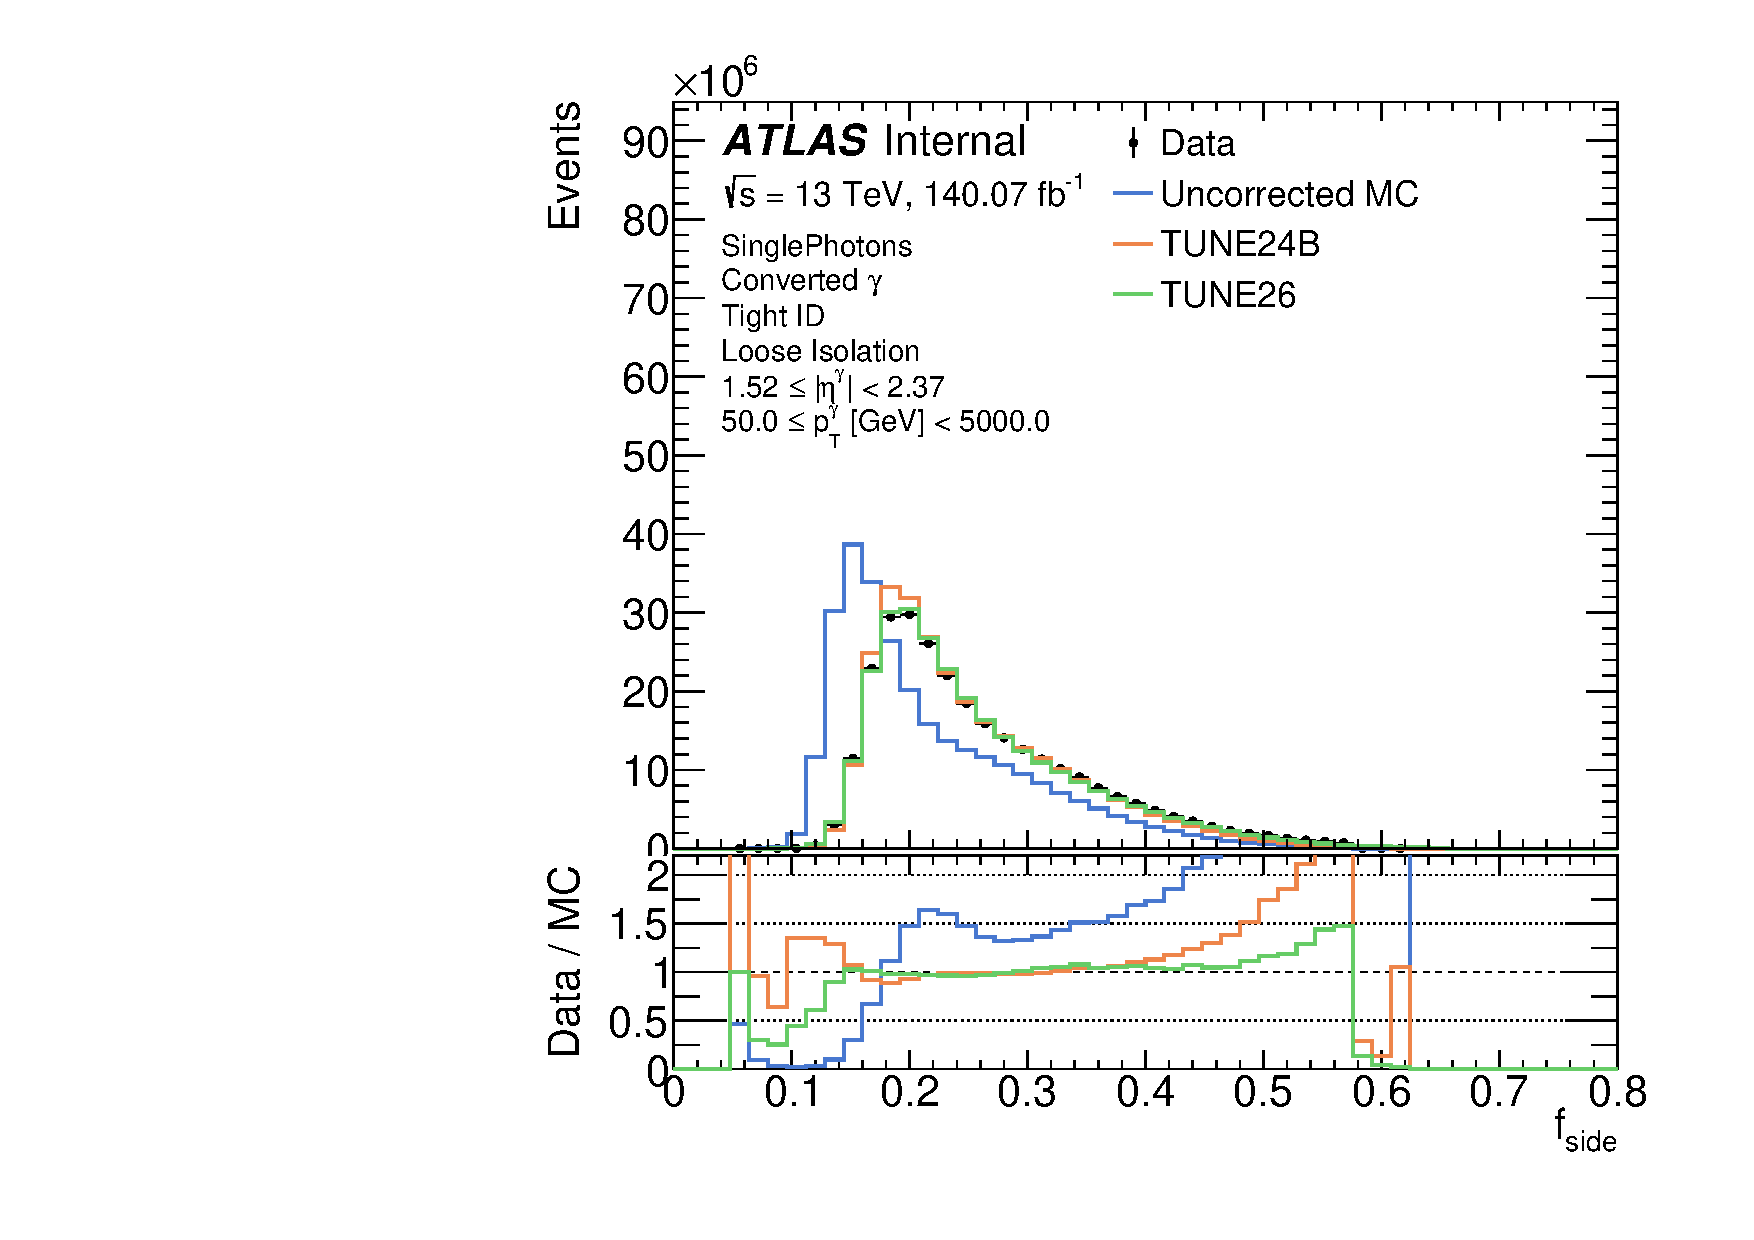
\includegraphics[width=\linewidth]{4_photonid/ffs/results/SP/corrections/c/ptFull/etaCoarse/can__correction__ph_fside__Isoloose_Idtight__c__ptFullpt0050p0__etaCoarseeta1p52}
        \caption{\fside, endcap.}
    \end{subfigure}
    \hfill
    \begin{subfigure}[h]{0.32\linewidth}
        \centering
        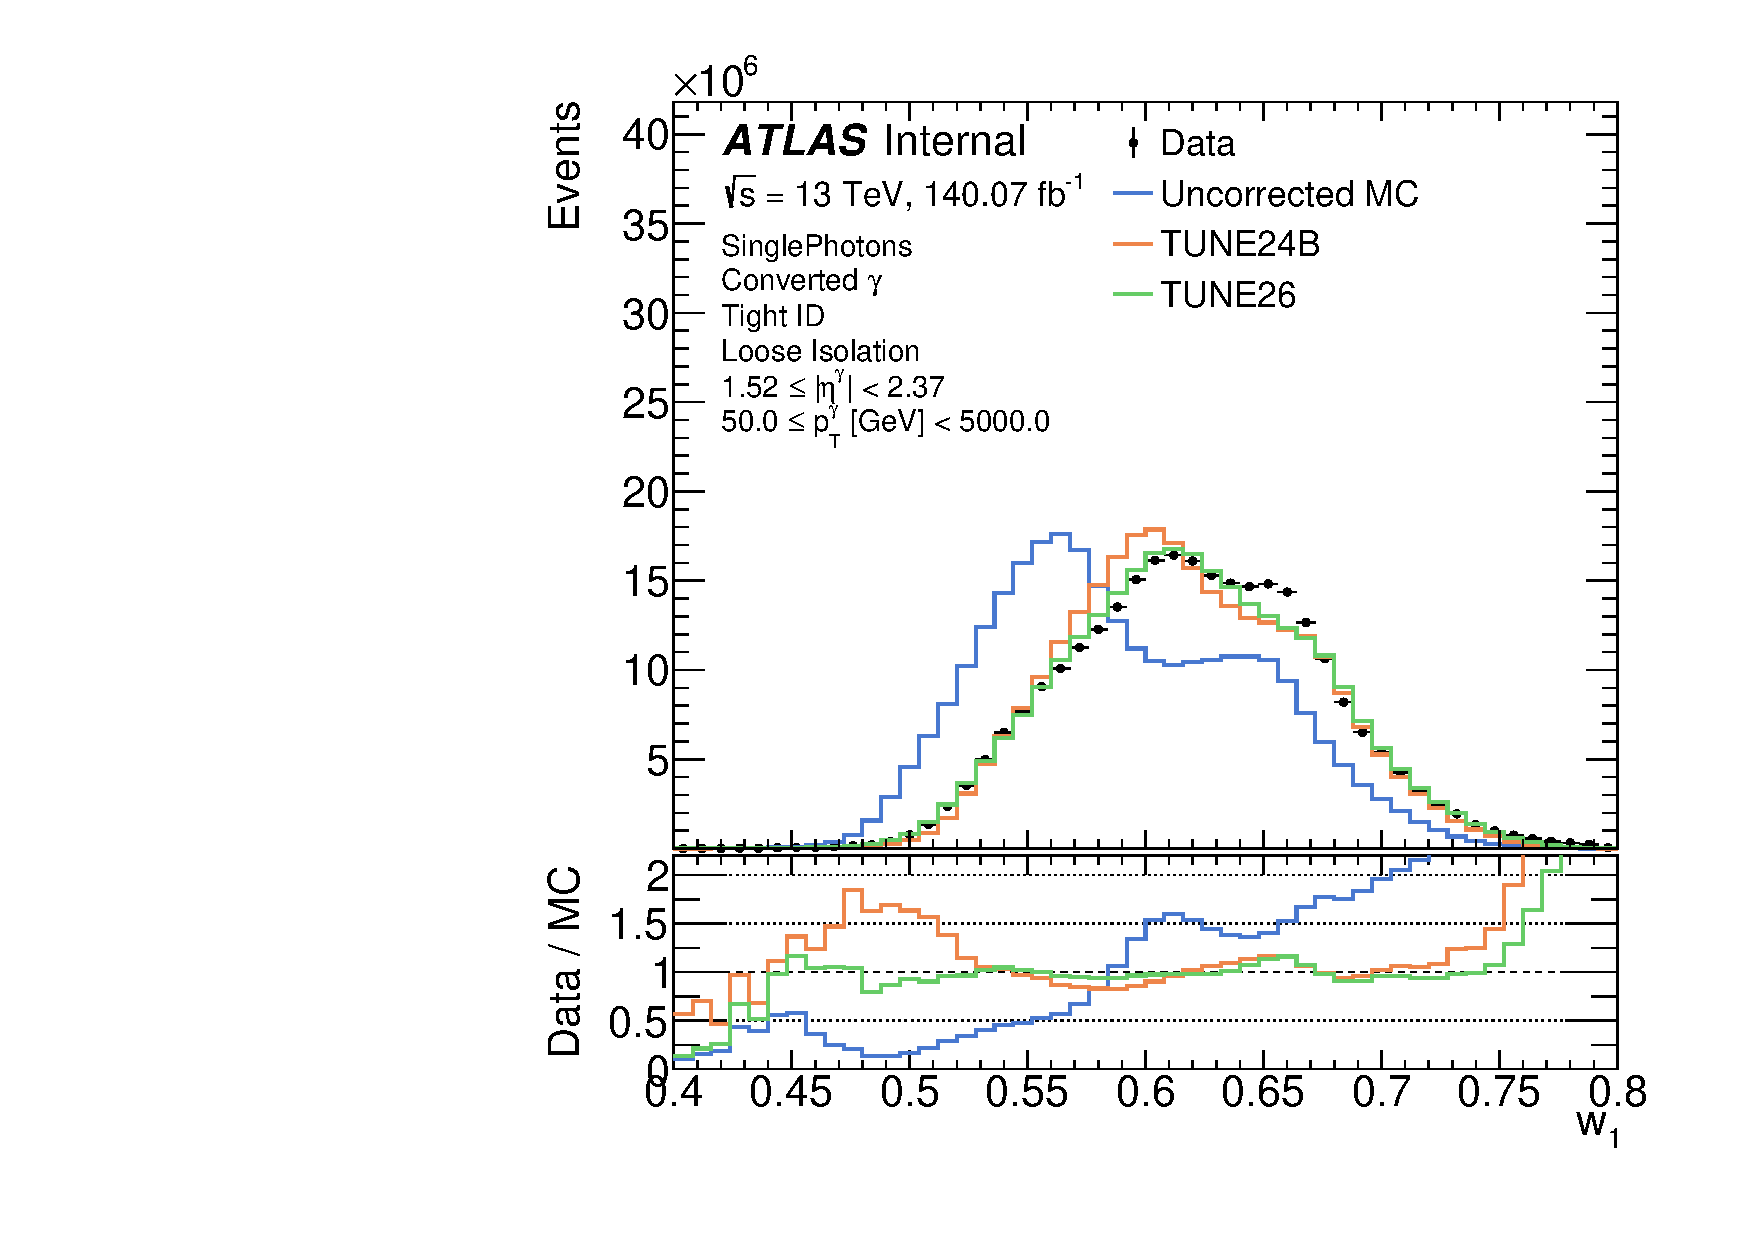
\includegraphics[width=\linewidth]{4_photonid/ffs/results/SP/corrections/c/ptFull/etaCoarse/can__correction__ph_w1__Isoloose_Idtight__c__ptFullpt0050p0__etaCoarseeta1p52}
        \caption{\wone, endcap.}
    \end{subfigure}
    \hfill
    \begin{subfigure}[h]{0.32\linewidth}
        \centering
        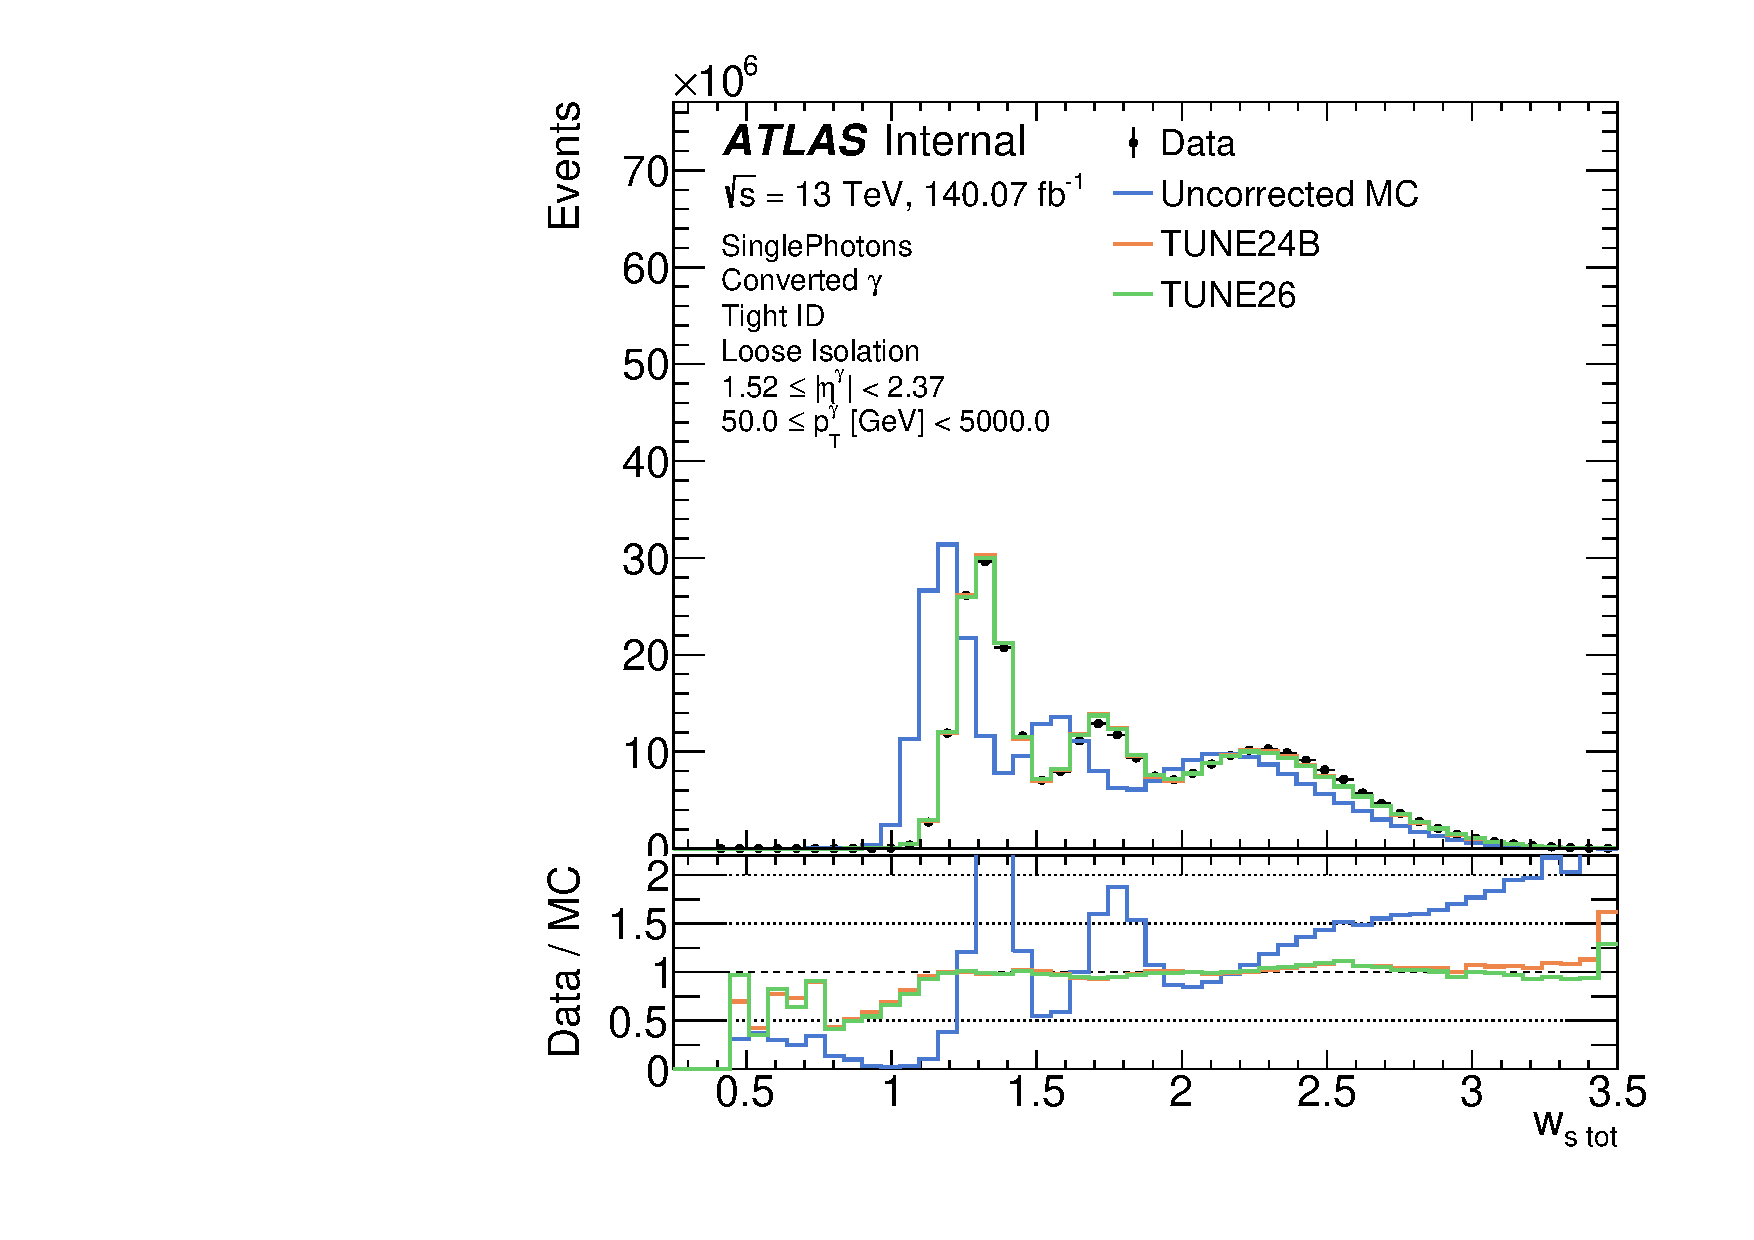
\includegraphics[width=\linewidth]{4_photonid/ffs/results/SP/corrections/c/ptFull/etaCoarse/can__correction__ph_wstot__Isoloose_Idtight__c__ptFullpt0050p0__etaCoarseeta1p52}
        \caption{\wstot, endcap.}
    \end{subfigure}\\
    \caption{Same as \Fig{\ref{fig:ss_corrections:ffs:results:ss_rz}} but with the \ac{SP} samples.}
    \label{fig:ss_corrections:ffs:results:ss_sp}
\end{figure}
























\section{Cell-based energy reweighting}
\label{sec:ss_corrections:cell_rw}

The design and functionality of the \ac{ATLAS} \ac{ECAL} was described in \Sect{\ref{subsubsec:atlas:atlas:cals:ecal}} as well as the process from which electrons and photons deposit their energies in the \ac{ECAL}: pair creation and bremsstrahlung radiation. Then, from these energy depositions in the \ac{ECAL} the \acp{SS} are built and used for photon identification. However, the fact that \ac{MC} and data \acp{SS} do not match, means that the energy depositions are different between these two, leading to a lower-level disagreement.

Although the \acf{FF} method described before led to an excellent improvement on the agreement between data and \ac{MC} distributions, it is still based on modifying high-level variables and all independently of each other. On the other hand, by directly correcting the cells' energy depositions in the simulation, a simultaneous fix to all the \acfp{SS} and any other variable computed from the energies would be acquired. This processes is what is known as cell-based energy reweighting.

The cell-based reweighting approach has been developed and tested initialy for electrons~\cite{thesis_khandoga}, and further tested for photons~\cite{thesis_belfkir}. For the electron's case, results have been very promising, where the second-layer \acp{SS} were substantially corrected. However, for photons, the same method that was used for electrons struggled, only working on average. Another approach to correct the simulation was based on matching data and simulated events, tested only on pseudo-data and technically complicated, but leading to better  improvements~\cite{thesis_belfkir}.

In the current section, a new way of correcting the cell energies in \ac{MC} is studied, using only the second layer of the \ac{ECAL}, for simplicity. The method shares similarities with the \ac{FF} method, making it easy to understand.
First, the special event selection used for this study is presented. An overview of the old method to correct energies is briefly discussed, and then a study on how this method is improved is presented.





\subsection{Event selection}
\label{subsec:ss_corrections:cell_rw:event_selection}

The studies presented in this section are carried out with the same dataset as used for the \ac{FF} calculation, described in \Sect{\ref{subsec:ss_corrections:ffs:samples}}. However, in this case, only the \ac{RZ} samples are used.
Events are selected as described in \Sect{\ref{subsec:pid_ss:pid:event_selection}}, using loose-isolated photons. Nevertheless, given that these studies rely on information on the second layer of the \ac{ECAL}, special selection on the cells needs to be taken into account.

When an electron or photon enters the calorimeter, its footprint in the second layer is a visible cluster of cells surrounding the most energetic and central one (also referred as \textit{hottest cell}). Clusters of \(7\times 11\) cells in \(\eta\times\phi\) are considered, shown in \Fig{\ref{fig:ss_corrections:cell_rw:event_selection:cluster:arrangement}} with the current cell arrangement used.
Approximately, 90\% of the energy of the cluster is shared amongst the 9 central cells, which are highlighted in blue in \Fig{\ref{fig:ss_corrections:cell_rw:event_selection:cluster:arrangement}}, and the average normalised energy for data is shown in \Fig{\ref{fig:ss_corrections:cell_rw:event_selection:cluster:energy}}, visualising how the energy is distributed.

\begin{figure}[ht!]
    \centering
    \begin{subfigure}[t]{0.49\linewidth}
        \centering
        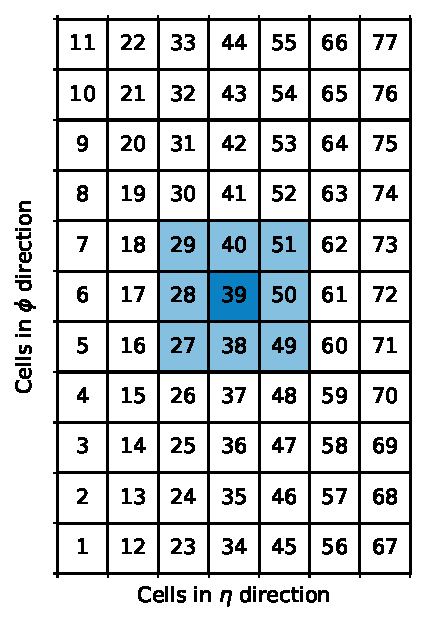
\includegraphics[width=0.5\linewidth]{4_photonid/cell_rw/cells_visualization}
        \caption{Cell arrangement showing the cell number. The hottest cell is cell number 39, and the neighbouring ones are highlighted in light blue.}
        \label{fig:ss_corrections:cell_rw:event_selection:cluster:arrangement}
    \end{subfigure}
    \hfill
    \begin{subfigure}[t]{0.49\linewidth}
        \centering
        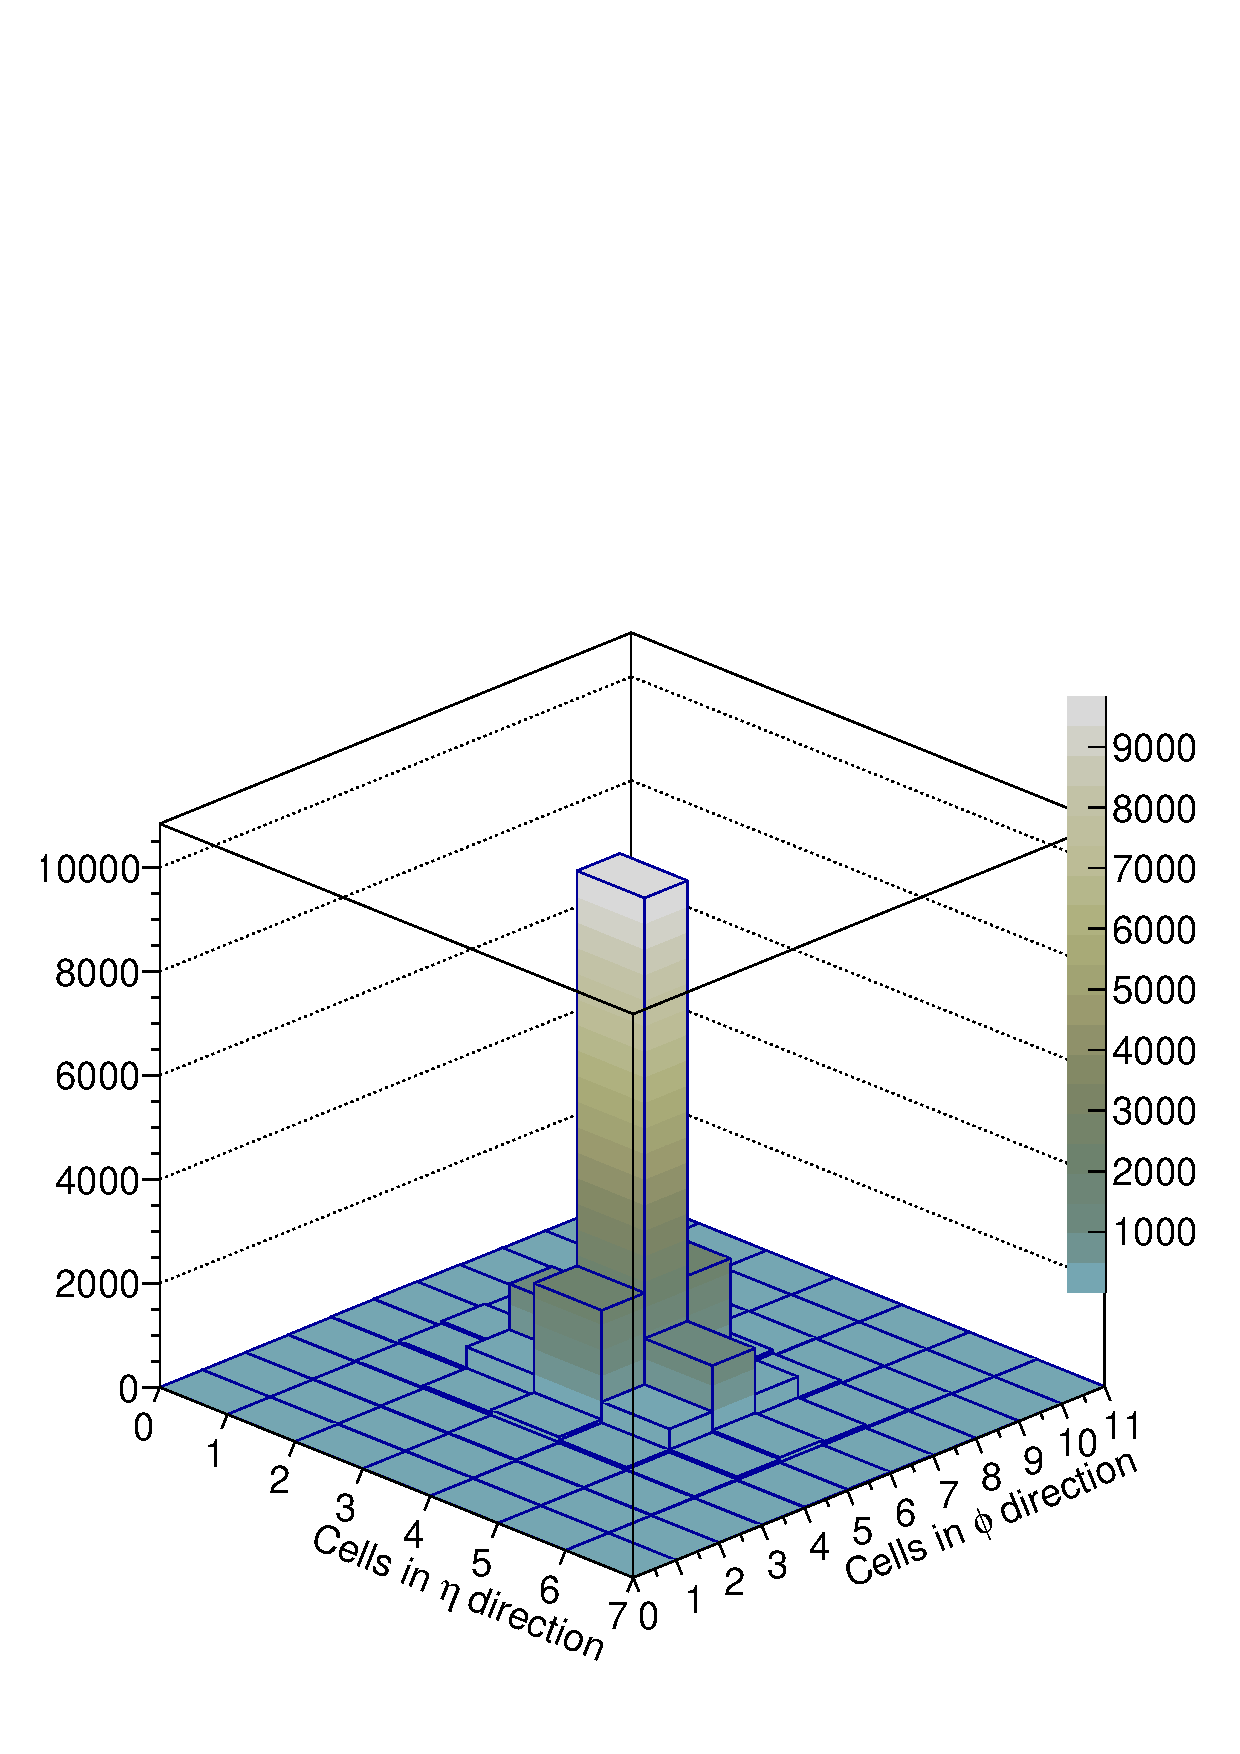
\includegraphics[width=0.8\linewidth]{4_photonid/cell_rw/cells-energy-u-etainclusive}
        \caption{Averge energy of cells in \(7\times 11\) clusters for data.}
        \label{fig:ss_corrections:cell_rw:event_selection:cluster:energy}
    \end{subfigure}
    \caption{Cells arrangement and average energy distribution amongst the clusters.}
    \label{fig:ss_corrections:cell_rw:event_selection:cluster}
\end{figure}

In this work, only events in which the clusters have the total of 77 cells are considered. Also, the events are required to have the central cell to be the most energetic.






\subsection{Calculation}
\label{subsec:ss_corrections:cell_rw:calculation}

\subsubsection{Early developments}
\label{subsubsec:ss_corrections:cell_rw:calculation:previous}

All events that pass the selection will have a cluster associated to it, each of one having \(N\) cells and each cell has an energy \(E_i\), for \(i=1,\dots,N\). For each event, in the first place, cluster energies are obtained as
\begin{equation*}
    E = \sum_{i=1}^{N} E_i.
\end{equation*}
which then are used to compute normalized cell energies \(e_i = E_i/E\). Distributions of these normalized energies are then obtained when considering all the events that pass selection, and their means are used to compute the corrections at each cell \(i\):
\begin{equation}
    \label{eq:ss_corrections:cell_rw:calculation:previous:old_corrections}
    \Delta_i = \overline{\left( \frac{ E_i^{\text{data}} }{ E^{\text{data}} } \right)} - \overline{\left( \frac{ E_i^{\text{MC}} }{ E^{\text{MC}} } \right)}
    = \bar e_i^{\text{data}} - \bar e_i^{\text{MC}}
\end{equation}
where \(E^{\text{data/MC}}\) are the cluster energies for data and \ac{MC} and, as mentioned above, the mean is done over all events that pass the selection. By definition these corrections coefficients sum to 0 over the whole cluster:
\begin{equation*}
    \sum_i \Delta_i = \sum_i \overline{\left( \frac{ E_i^{\text{data}} }{ E^{\text{data}} } \right)} - \sum_i \overline{\left( \frac{ E_i^{\text{MC}} }{ E^{\text{MC}} } \right)}
    = \overline{\sum_i \frac{ E_i^{\text{data}} }{ E^{\text{data}} }} - \overline{\sum_i \frac{ E_i^{\text{MC}} }{ E^{\text{MC}} }}
    = 1 - 1 = 0
\end{equation*}
Then a cell energy is corrected as:
\begin{equation}
    \label{eq:ss_corrections:cell_rw:calculation:previous:correction_method}
    E_i^{\text{MC-RW}} = E_i^{\text{MC}} + \Delta_i E^{\text{MC}},
\end{equation}
which is translated into shifting the cell energy divided by the cluster energy \(E^{\text{MC}}\) (from now on called normalized cell energy, \(e_i^{\text{MC}}\)) by an amount of \(\Delta\), so data and \ac{MC} distributions' means match. For the early studies on photons, reweights were calculated separately for unconverted and converted photons, and they were also binned in \(\abseta\):
\[
    \abseta: [0, 0.2, 0.4, 0.6, 0.8, 1.0, 1.2, 1.3, 1.37, 1.52, 1.6, 1.8, 2.0, 2.2, 2.37]
\]

Because the corrections coefficients sum to zero, this method also implies that the cluster energy remains constant throughout the reweighting procedure:
\begin{equation*}
    E^{\text{MC-RW}} \equiv \sum_i E_i^{\text{MC-RW}}
    = \sum_i E_i^{\text{MC}} + \sum_i \Delta_i E^{\text{MC}} = E^{\text{MC}} + E^{\text{MC}} \sum_i \Delta_i = E^{\text{MC}}
\end{equation*}

The corrections can be visualized as 2-dimensional matrices, as seen in \Fig{\ref{fig:ss_corrections:cell_rw:calculation:previous:reweights}}, and therefore the reweighting procedure is developed using 2-dimensional histograms. For the case of working with the calorimeter layer 2, clusters of 77 cells (\(\eta\times\phi=7\times11\)) are used.

\begin{figure}[htbp]
    \centering
    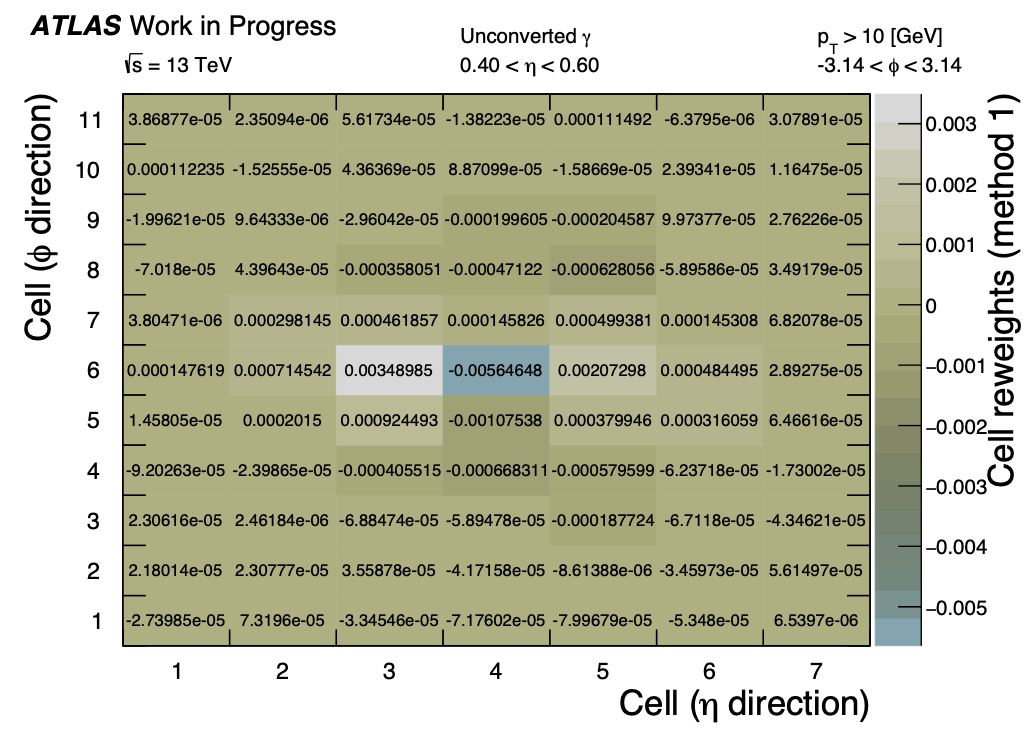
\includegraphics[width=0.48\linewidth]{4_photonid/cell_rw/old_method/reweights_method1u_ptInclusive_eta040_phiInclusive}
    \caption{Energy reweights to be applied to \ac{MC} cells, for unconverted photons with \(0.4<\abseta<0.6\). \fixme{fix luminosity}}
    \label{fig:ss_corrections:cell_rw:calculation:previous:reweights}
\end{figure}

The \acp{SS} computed using the second-layer information are \reta, \rphi and \weta, which can be calculated from energy deposits from the relations:
\begin{gather*}
    \reta = \frac{E_{3\times 7}}{E_{7\times 7}}\\
    \rphi = \frac{E_{3\times 3}}{E_{7\times 3}}\\
    \weta = \sqrt{\frac{\sum_i E_i \eta^2_i}{\sum_i E_i} - \left( \frac{\sum_i E_i \eta_i}{\sum_i E_i} \right)^2}
\end{gather*}
where \(E_{i\times j}\) is the summed cell energy in a region \(\eta\times\phi=i\times j\) cells around the central cell. It was shown in the previous studies~\cite{thesis_belfkir} that this method only corrects the shower shapes in average, but differences on the shape remain. This is due to the fact that this method only corrects the means of the energies distributions, by redistributing the energies amongst the cells. However, these energy distributions still present differences, specially regarding the shapes, leading to a very similar situation to what has been seen for the \acp{FF}. In this manner, a very similar approach of further correcting the means and widths of the normalised energies distributions can be employed.


% \reta and \rphi \acp{SS} are showed in \Fig{\ref{fig:ss_corrections:cell_rw:calculation:previous:ss}}. Present results manage to reproduce the same behaviours for both \acp{SS}, indicating an improvement in \reta while no big changes are seen for \rphi. This means that the reweighting method used for electrons does not work correctly for photons, although stepping into the right direction.


% \begin{figure}[ht!]
%     \centering
%     \begin{subfigure}[h]{0.49\linewidth}
%         \centering
%         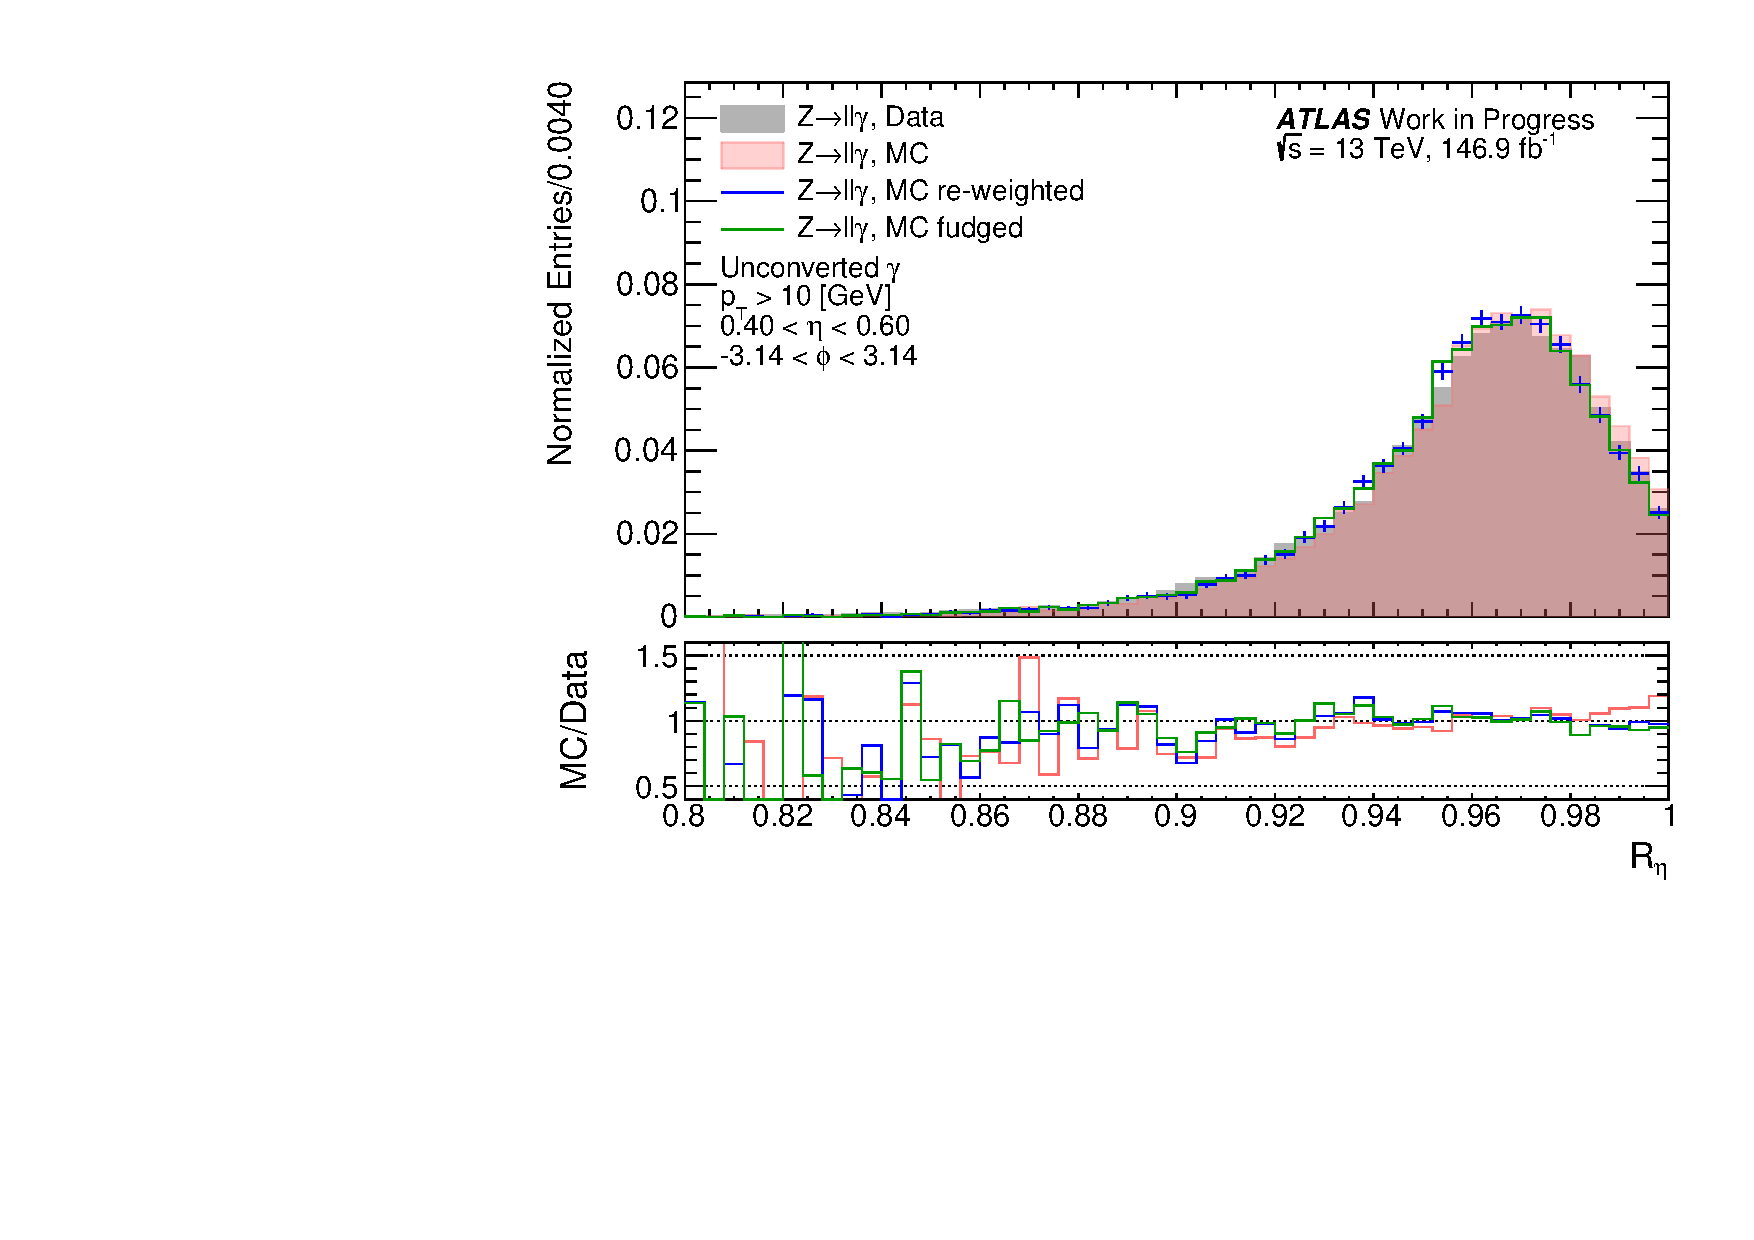
\includegraphics[width=\linewidth]{4_photonid/cell_rw/old_method/ss_Reta_RW_u_ptInclusive_eta040_phiInclusive}
%         \caption{\reta}
%     \end{subfigure}
%     \hfill
%     \begin{subfigure}[h]{0.49\linewidth}
%         \centering
%         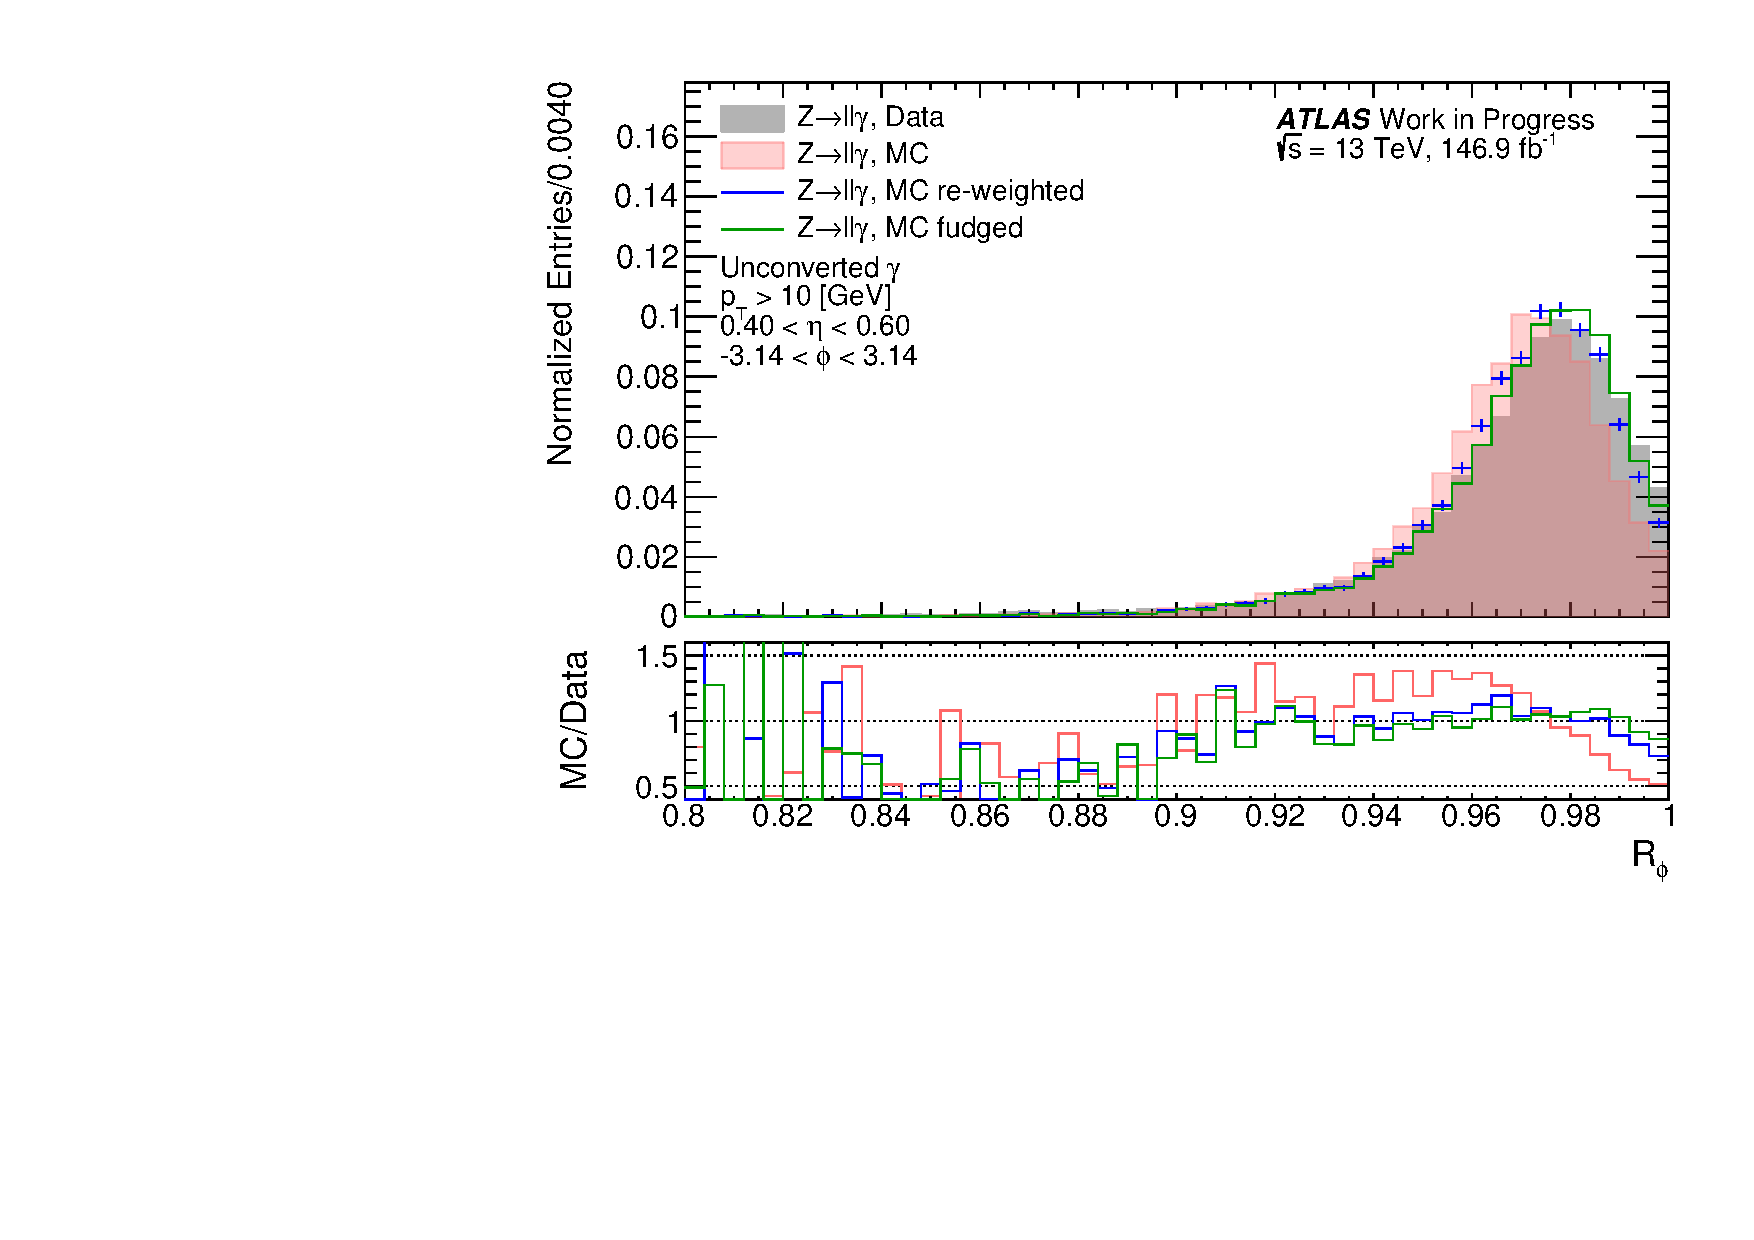
\includegraphics[width=\linewidth]{4_photonid/cell_rw/old_method/ss_Rphi_RW_u_ptInclusive_eta040_phiInclusive}
%         \caption{\rphi}
%     \end{subfigure}
%     \caption{Comparison of \ac{SS} between data (grey histogram) and uncorrected (red histogram) fudged (green line) and re-weighted (blue line) \ac{MC} simulation. The bottom pad of the figures show the ratio of simulation over data.}
%     \label{fig:ss_corrections:cell_rw:calculation:previous:ss}
% \end{figure}



\subsubsection{New re-weighting method}

This new method aims to correct both the mean and variance of normalized cell energies distributions by applying shifts and stretches. Similar to the approach followed for \acp{SS}, a first approximation for shift and stretch values of the energy distributions is to compute means and root mean squares (RMS) of them at each cell, respectively. Then, reweighted normalized cell energies can be obtained as
\begin{equation}
    \label{eq:ss_corrections:cell_rw:calculation:new:normalized_e}
    e_i^{\text{MC-RW}} = \frac{\text{RMS}_{e,i}^{\text{data}}}{\text{RMS}_{e,i}^{\text{MC}}} \left( e_i^{\text{MC}} - \bar e_i^{\text{MC}} \right) + \bar e_i^{\text{data}},
\end{equation}
where the subindex \(e\) indicates that the RMS is calculated from normalized cell energy distributions and \(i\) runs over all cells in the cluster.

Since the normalized cell energy at cell \(i\) can be calculated as \(e_i^{j} = E_i^{j} / E^{j}\), for \(j=\)MC-RW, MC and data, and it is required to have the same cluster energy after the reweighting procedure (\(E^{\text{MC-RW}} = E^{\text{MC}}\)). Multiplying \Eqn{\ref{eq:ss_corrections:cell_rw:calculation:new:normalized_e}} by \(E^{\text{MC-RW}}\) it is possible to arrive at an expression for \(E_i^{\text{MC-RW}}\):
\begin{equation}
    \label{eq:ss_corrections:cell_rw:calculation:new:correction_method}
    E_i^{\text{MC-RW}} = \frac{\text{RMS}_{e,i}^{\text{data}}}{\text{RMS}_{e,i}^{\text{MC}}} E_i^{\text{MC}} + \left( \bar e_i^{\text{data}} - \frac{\text{RMS}_{e,i}^{\text{data}}}{\text{RMS}_{e,i}^{\text{MC}}} \bar e_i^{\text{MC}} \right) E^{\text{MC}}.
\end{equation}
Comparing \Eqn{\ref{eq:ss_corrections:cell_rw:calculation:new:correction_method}} to \Eqn{\ref{eq:ss_corrections:cell_rw:calculation:previous:correction_method}}, it is observed that \(E_i^{\text{MC}}\) is now multiplied by a stretch factor, and a similar shift is applied to the normalized cell energy distribution but with modifications introduced by the stretch:
\begin{equation*}
    \begin{split}
        \text{stretch:}& \qquad 1 \to \frac{\text{RMS}_{e,i}^{\text{data}}}{\text{RMS}_{e,i}^{\text{MC}}}\\
        \text{shift:}& \qquad \bar e_i^{\text{data}} - \bar e_i^{\text{MC}} \to \bar e_i^{\text{data}} - \frac{\text{RMS}_{e,i}^{\text{data}}}{\text{RMS}_{e,i}^{\text{MC}}} \bar e_i^{\text{MC}}
    \end{split}
\end{equation*}

Finally, to guarantee that the cluster energy remains constant, cell energies are re-scaled by \(\sum_i E_i^{\text{MC}} / \sum_i E_i^{\text{MC-RW}}\). As a result of this procedure, two reweights matrices are needed, and one example of them is presented in \Fig{\ref{fig:ss_corrections:cell_rw:calculation:new:reweights}}.
For what follows, this new method is applied to correct the cell energies, and it is computed inclusively in \pt and \abseta, only separating between unconverted and converted photons.

\begin{figure}[ht!]
    \centering
    \begin{subfigure}[h]{0.49\linewidth}
        \centering
        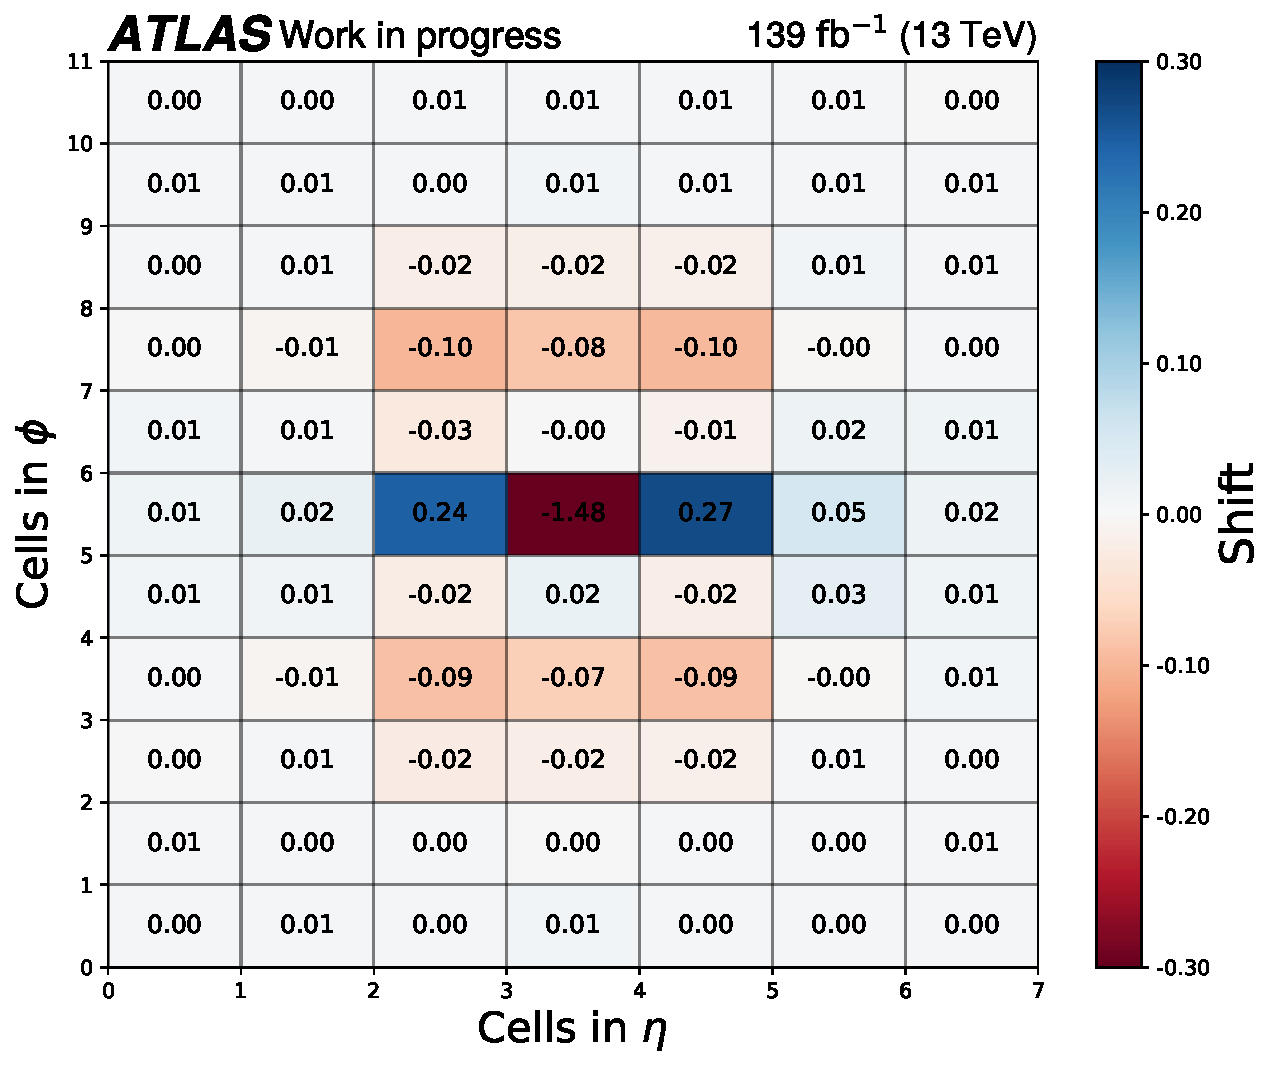
\includegraphics[width=\linewidth]{4_photonid/cell_rw/results/h_u_shift_mpl}
        \caption{Shift correction}
    \end{subfigure}
    \hfill
    \begin{subfigure}[h]{0.49\linewidth}
        \centering
        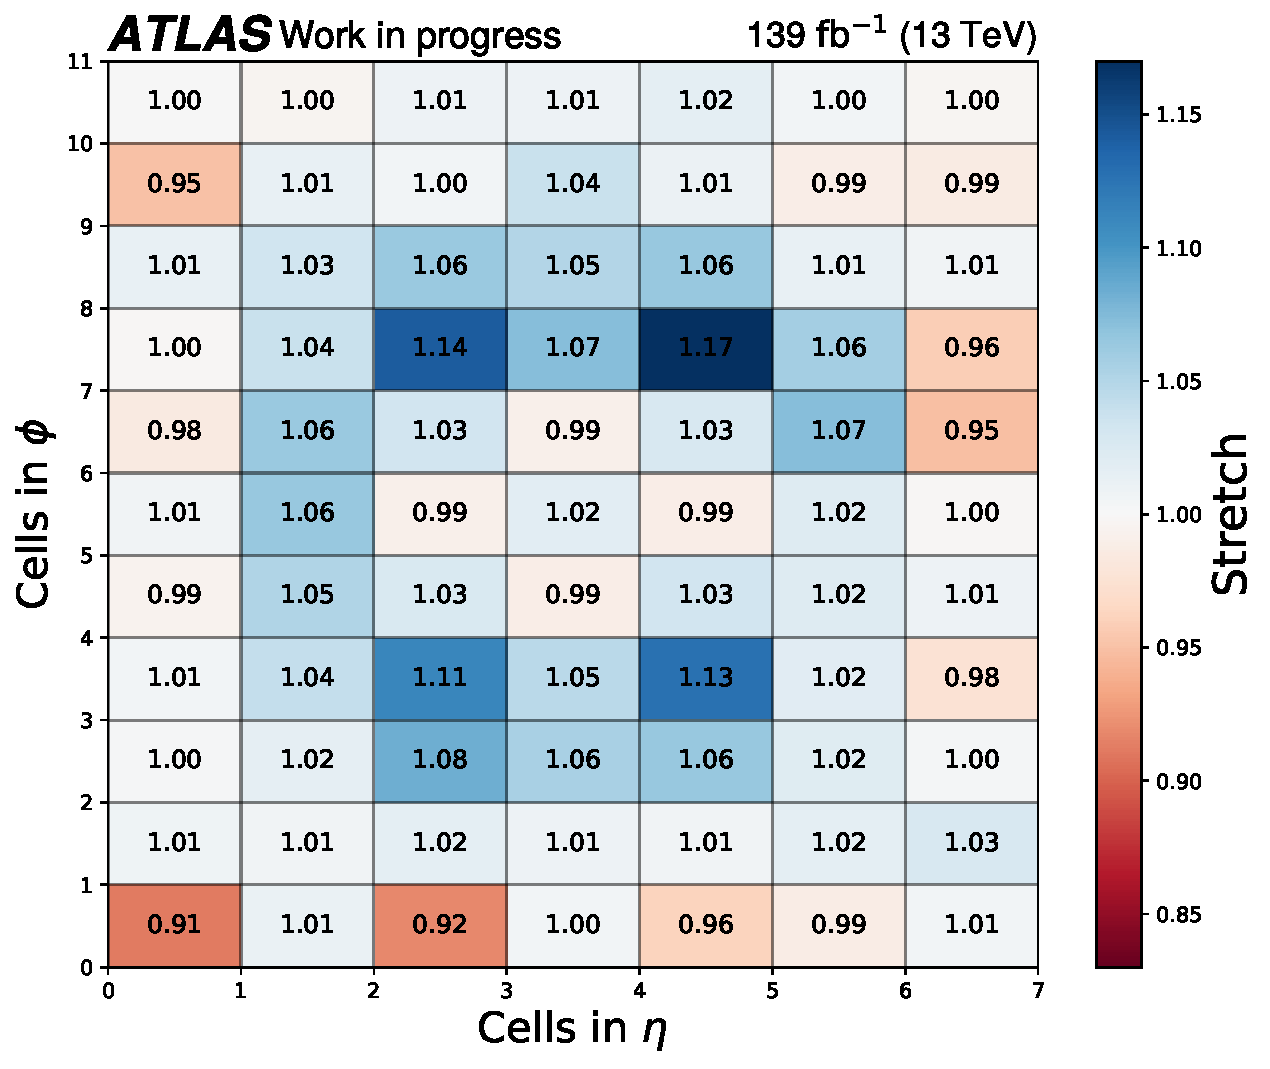
\includegraphics[width=\linewidth]{4_photonid/cell_rw/results/h_u_stretch_mpl}
        \caption{Stretch correction}
    \end{subfigure}
    \caption{Example of two reweights matrices, using shift (left) and stretches (right) corrections. Shown results correspond to unconverted photons. The shift values are multiplied by a factor of 100 to improve visualisation.}
    \label{fig:ss_corrections:cell_rw:calculation:new:reweights}
\end{figure}









\subsection{Results}
\label{subsec:ss_corrections:cell_rw:results}

\Fig{\ref{fig:ss_corrections:cell_rw:calculation:new:reweights}} shows the shift and stretch reweighting matrices for unconverted photons. It can be noted that the major shift correction is done in the central cell, where the shift corresponds to a negative value. Negative shifts to the normalised cell energy means that energy must be removed from the central cell, and distributed to the neighbouring ones, as seen from the positive shifts values in the closest cells. Regarding stretch values, a rather symmetric distribution of values is observed with respect to the central cell.

Using these correction factors to the normalised energies to each cell, in \Fig{\ref{fig:ss_corrections:cell_rw:results:cells}}, the resulting cell energy distributions are displayed for cells 28, 39 and 50~\footnote{As shown in \Fig{\ref{fig:ss_corrections:cell_rw:event_selection:cluster:arrangement}}, cell number 39 is the central one, while cell 28 and 50 are to the left and right, respectively, in the \(\eta\) direction.}. The new reweighting method achieves greats improvements on the agreement between data and MC. The reweighting method does well correcting tails of the distributions for all cells, as well as the peaks of them, which can be seen specially for cell 28.

\begin{figure}[ht!]
    \centering
    \begin{subfigure}[h]{0.32\linewidth}
        \centering
        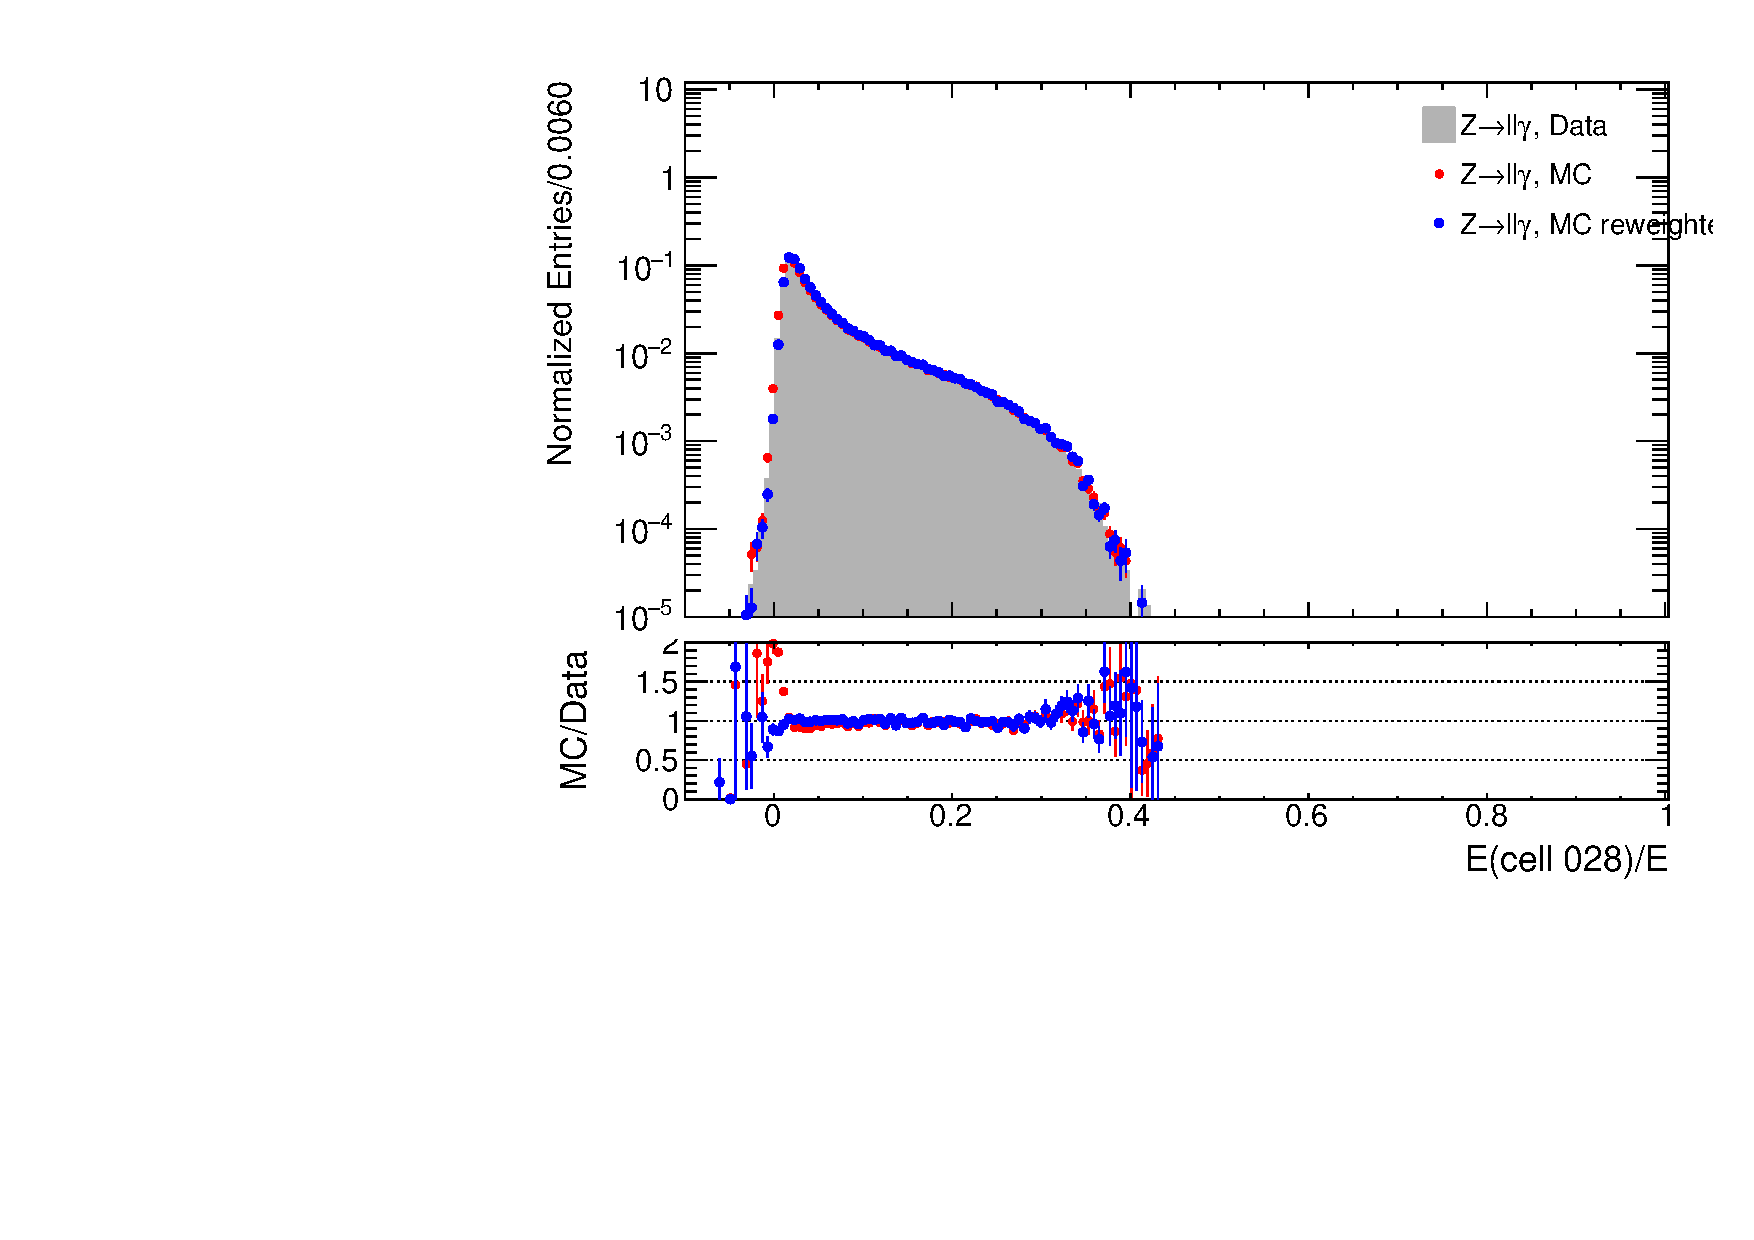
\includegraphics[width=\linewidth]{4_photonid/cell_rw/results/cells/c__u__L2_e_cell_028_normTo1}
        \caption{Cell 28}
    \end{subfigure}
    \hfill
    \begin{subfigure}[h]{0.32\linewidth}
        \centering
        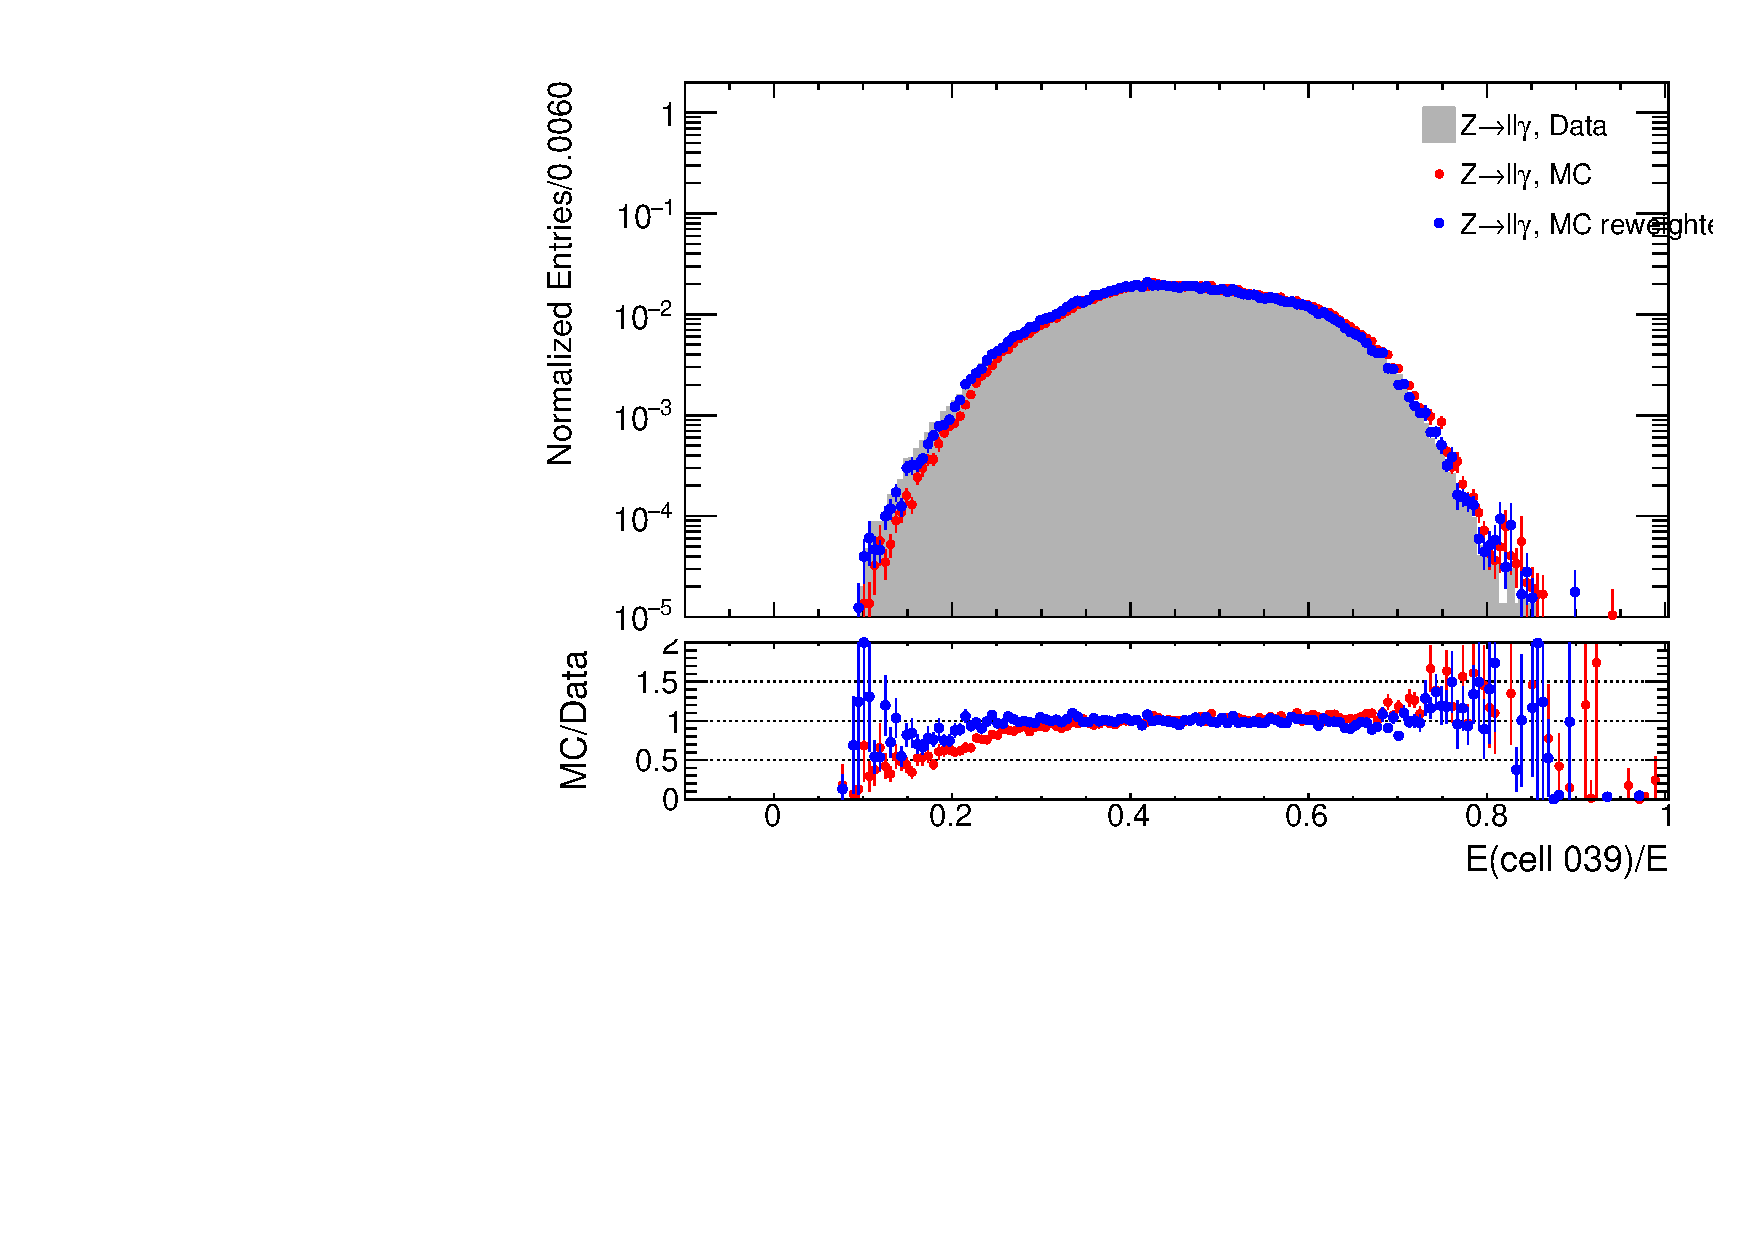
\includegraphics[width=\linewidth]{4_photonid/cell_rw/results/cells/c__u__L2_e_cell_039_normTo1}
        \caption{Cell 39}
    \end{subfigure}
    \hfill
    \begin{subfigure}[h]{0.32\linewidth}
        \centering
        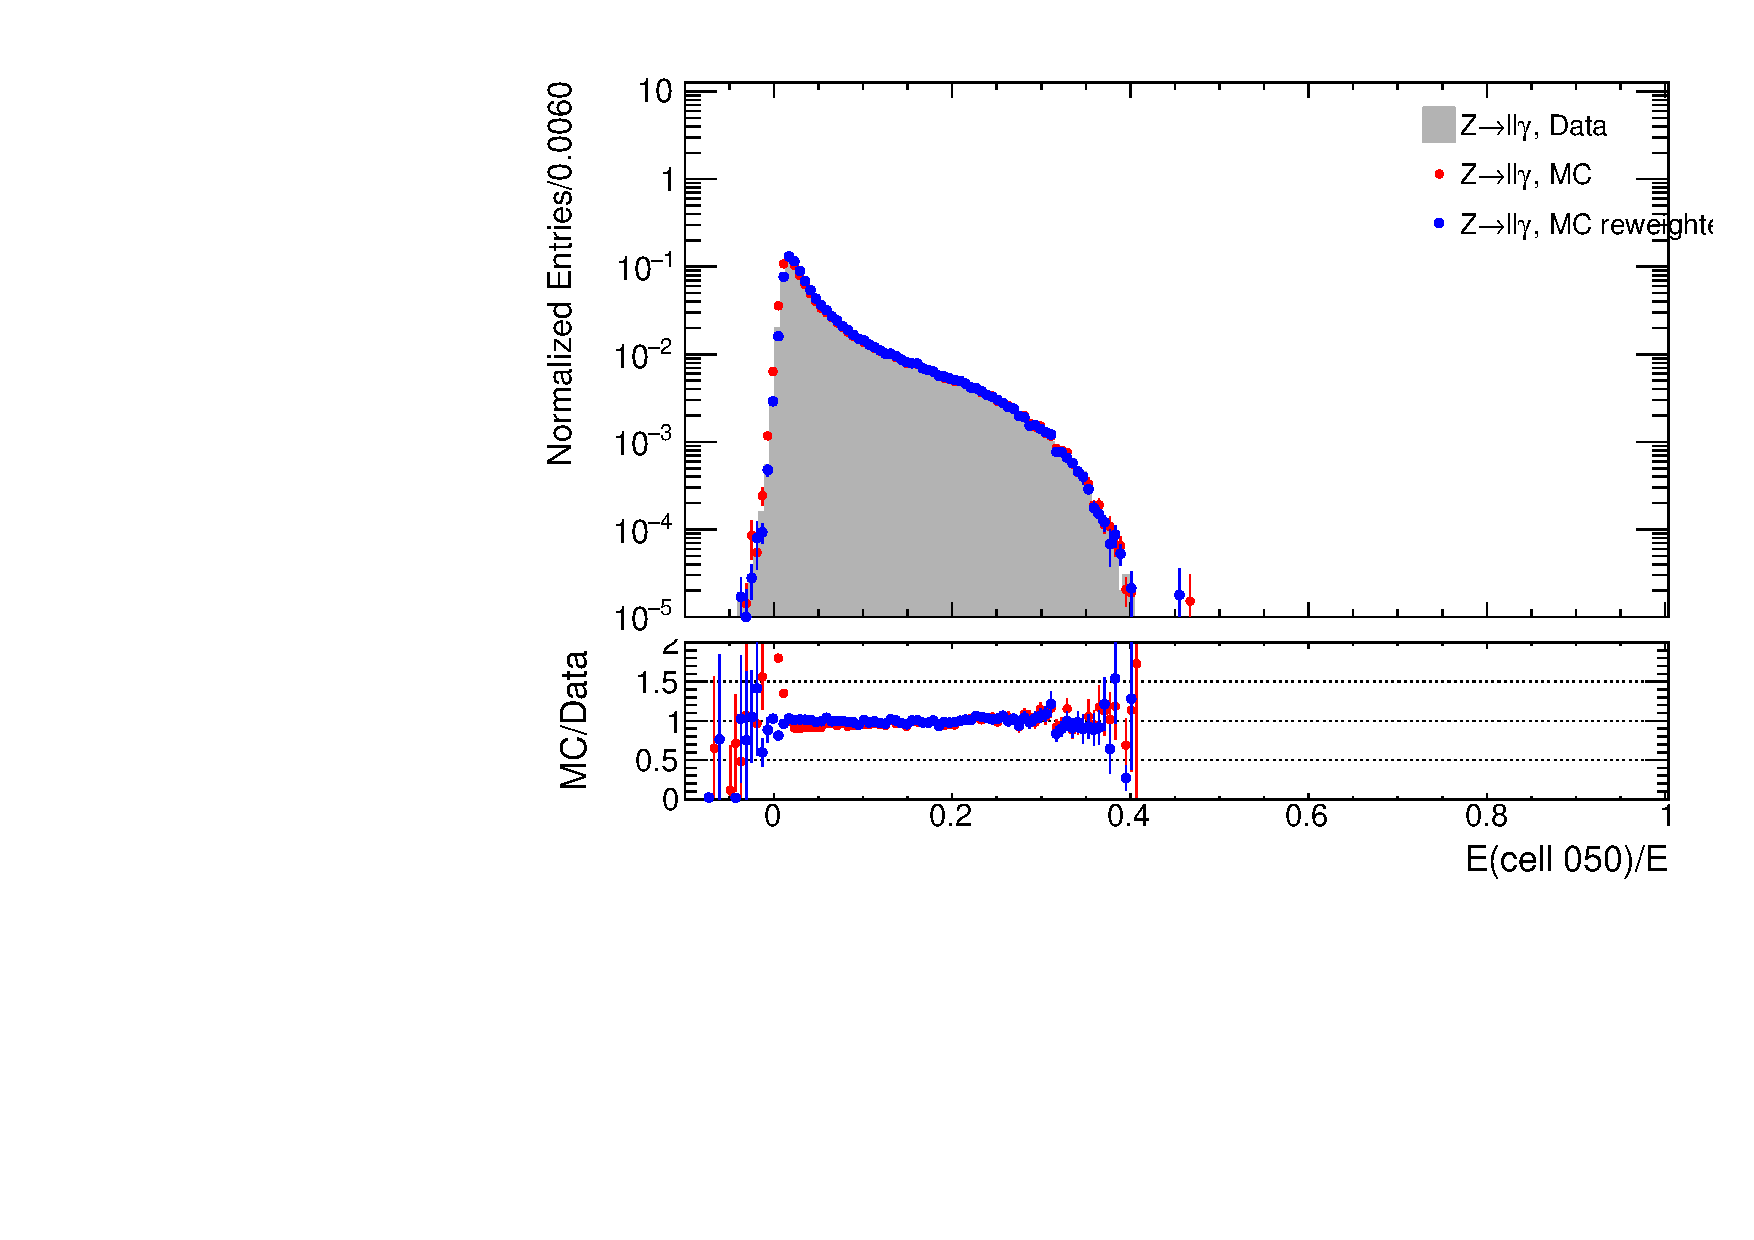
\includegraphics[width=\linewidth]{4_photonid/cell_rw/results/cells/c__u__L2_e_cell_050_normTo1}
        \caption{Cell 50}
    \end{subfigure}
    \caption{Normalized cell energy distributions for cells 28, 39 and 50 of the cluster using unconverted photons. Blue and red points correspond to the reweighted and original \ac{MC} distributions, respectively, while the grey histogram represents data.}
    \label{fig:ss_corrections:cell_rw:results:cells}
\end{figure}



To assess the behaviour of the reweighting procedure applied to the \acp{SS} of the second \ac{ECAL} layer, in \Fig{\ref{fig:ss_corrections:cell_rw:results:ss}} the comparison of the methods for correcting the \reta, \rphi and \weta \acp{SS} are shown. In the three cases, an improvement over the uncorrected \ac{MC} is observed, specially for the \rphi and \weta variables, but the cell-based energy reweighting method for unconverted photons does not reach the level of agreement with data as the \acp{FF}, which has been shown to provide an excellent match with data. Nevertheless, there is almost no difference seen between the reweighting and the \ac{FF} method for converted photons, indicating that there is room for improvement on the corrections.


\begin{figure}[ht!]
    \centering
    \begin{subfigure}[h]{0.32\linewidth}
        \centering
        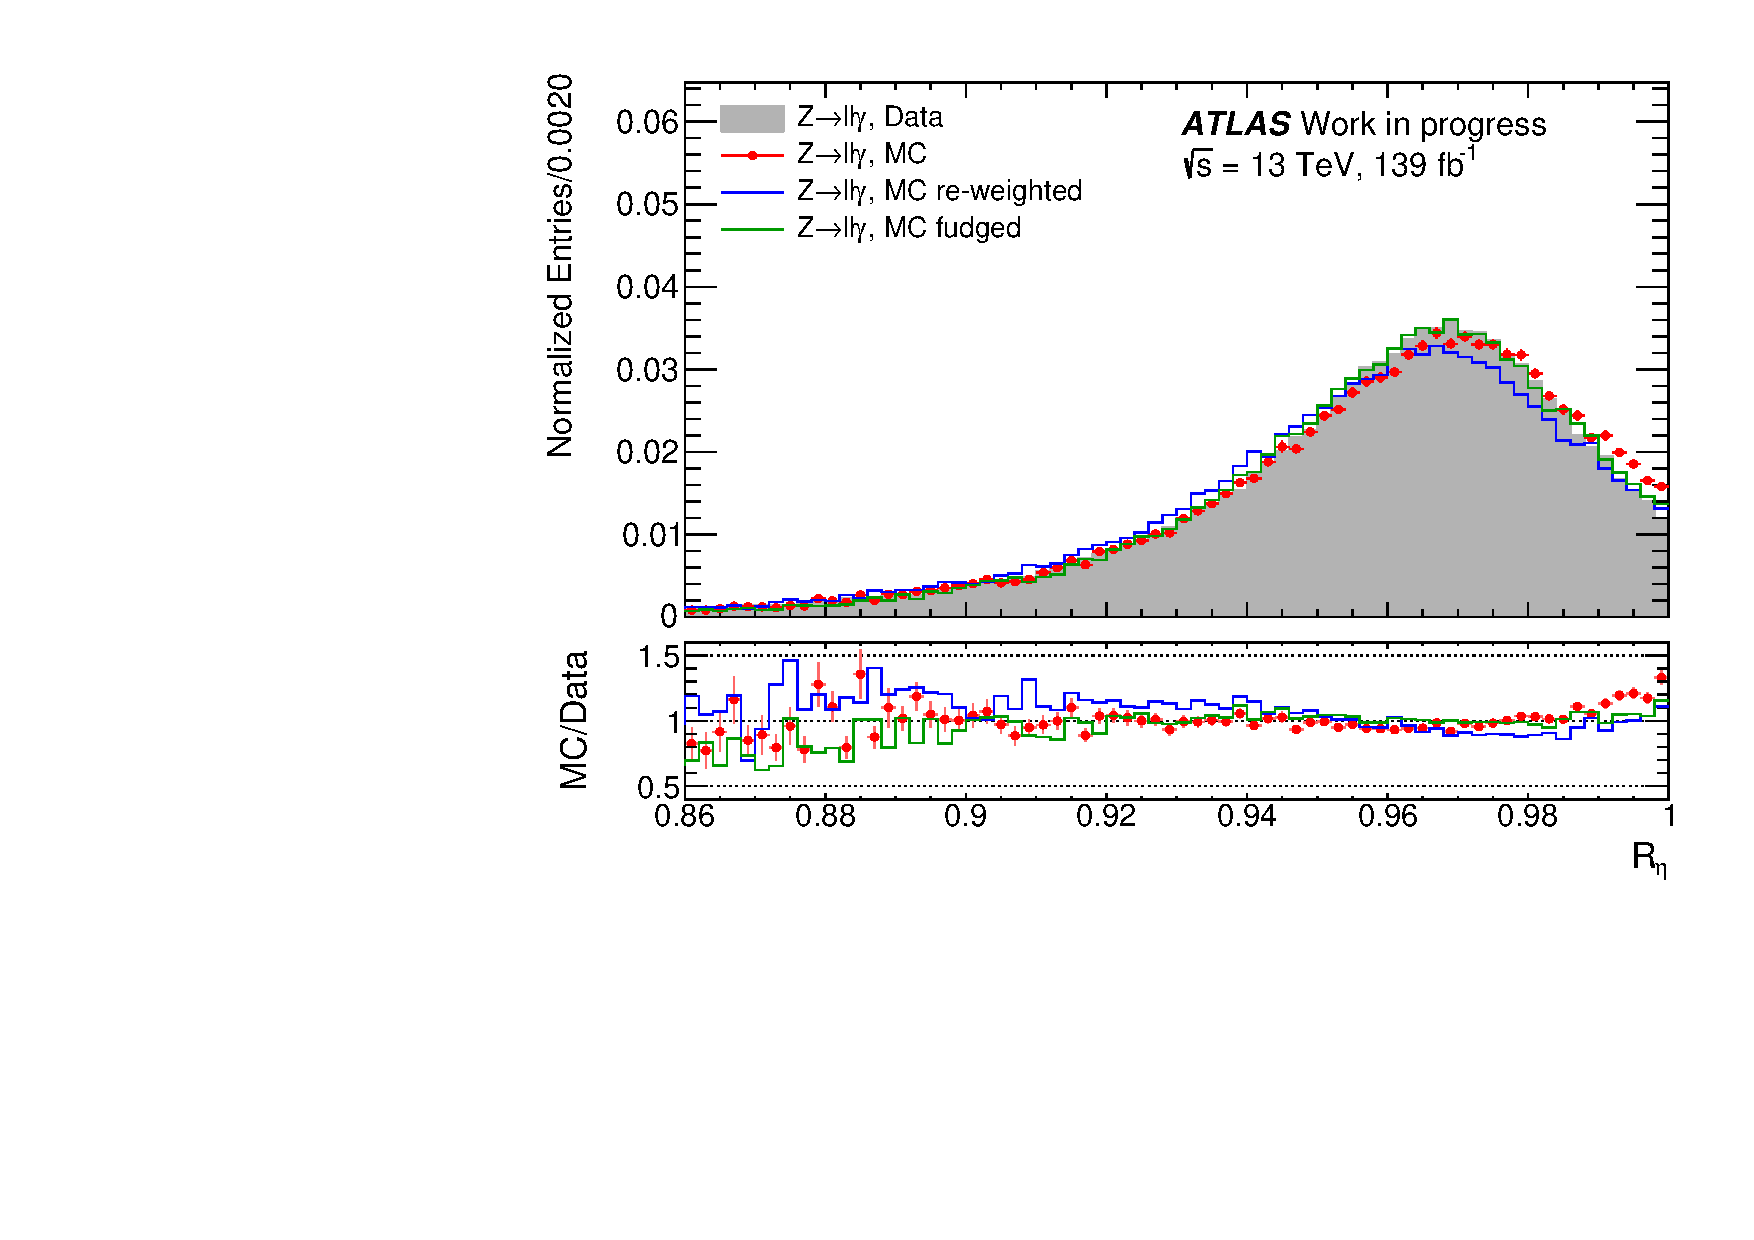
\includegraphics[width=\linewidth]{4_photonid/cell_rw/results/ss/c__u_eta00__ss_Reta}
        \caption{\reta, unconverted photons}
    \end{subfigure}
    \hfill
    \begin{subfigure}[h]{0.32\linewidth}
        \centering
        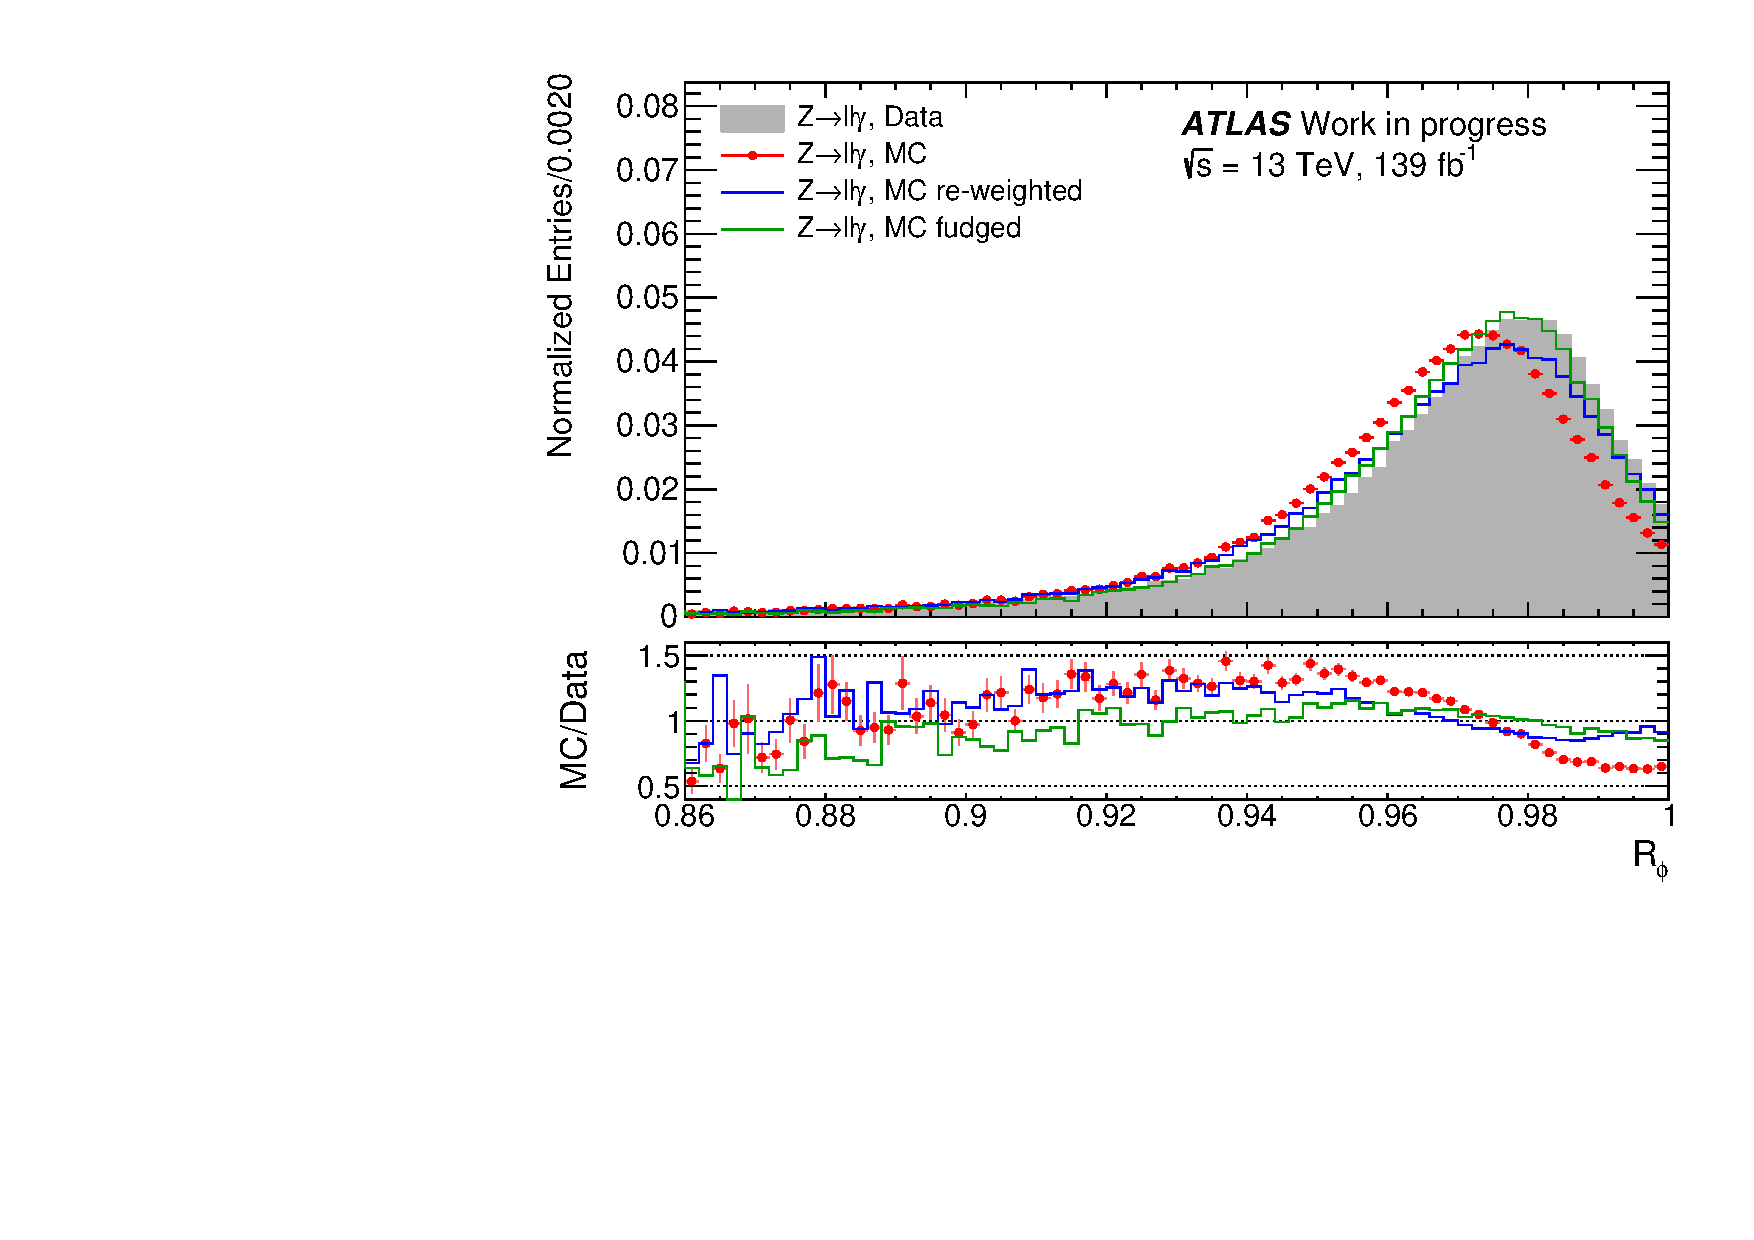
\includegraphics[width=\linewidth]{4_photonid/cell_rw/results/ss/c__u_eta00__ss_Rphi}
        \caption{\rphi, unconverted photons}
    \end{subfigure}
    \begin{subfigure}[h]{0.32\linewidth}
        \centering
        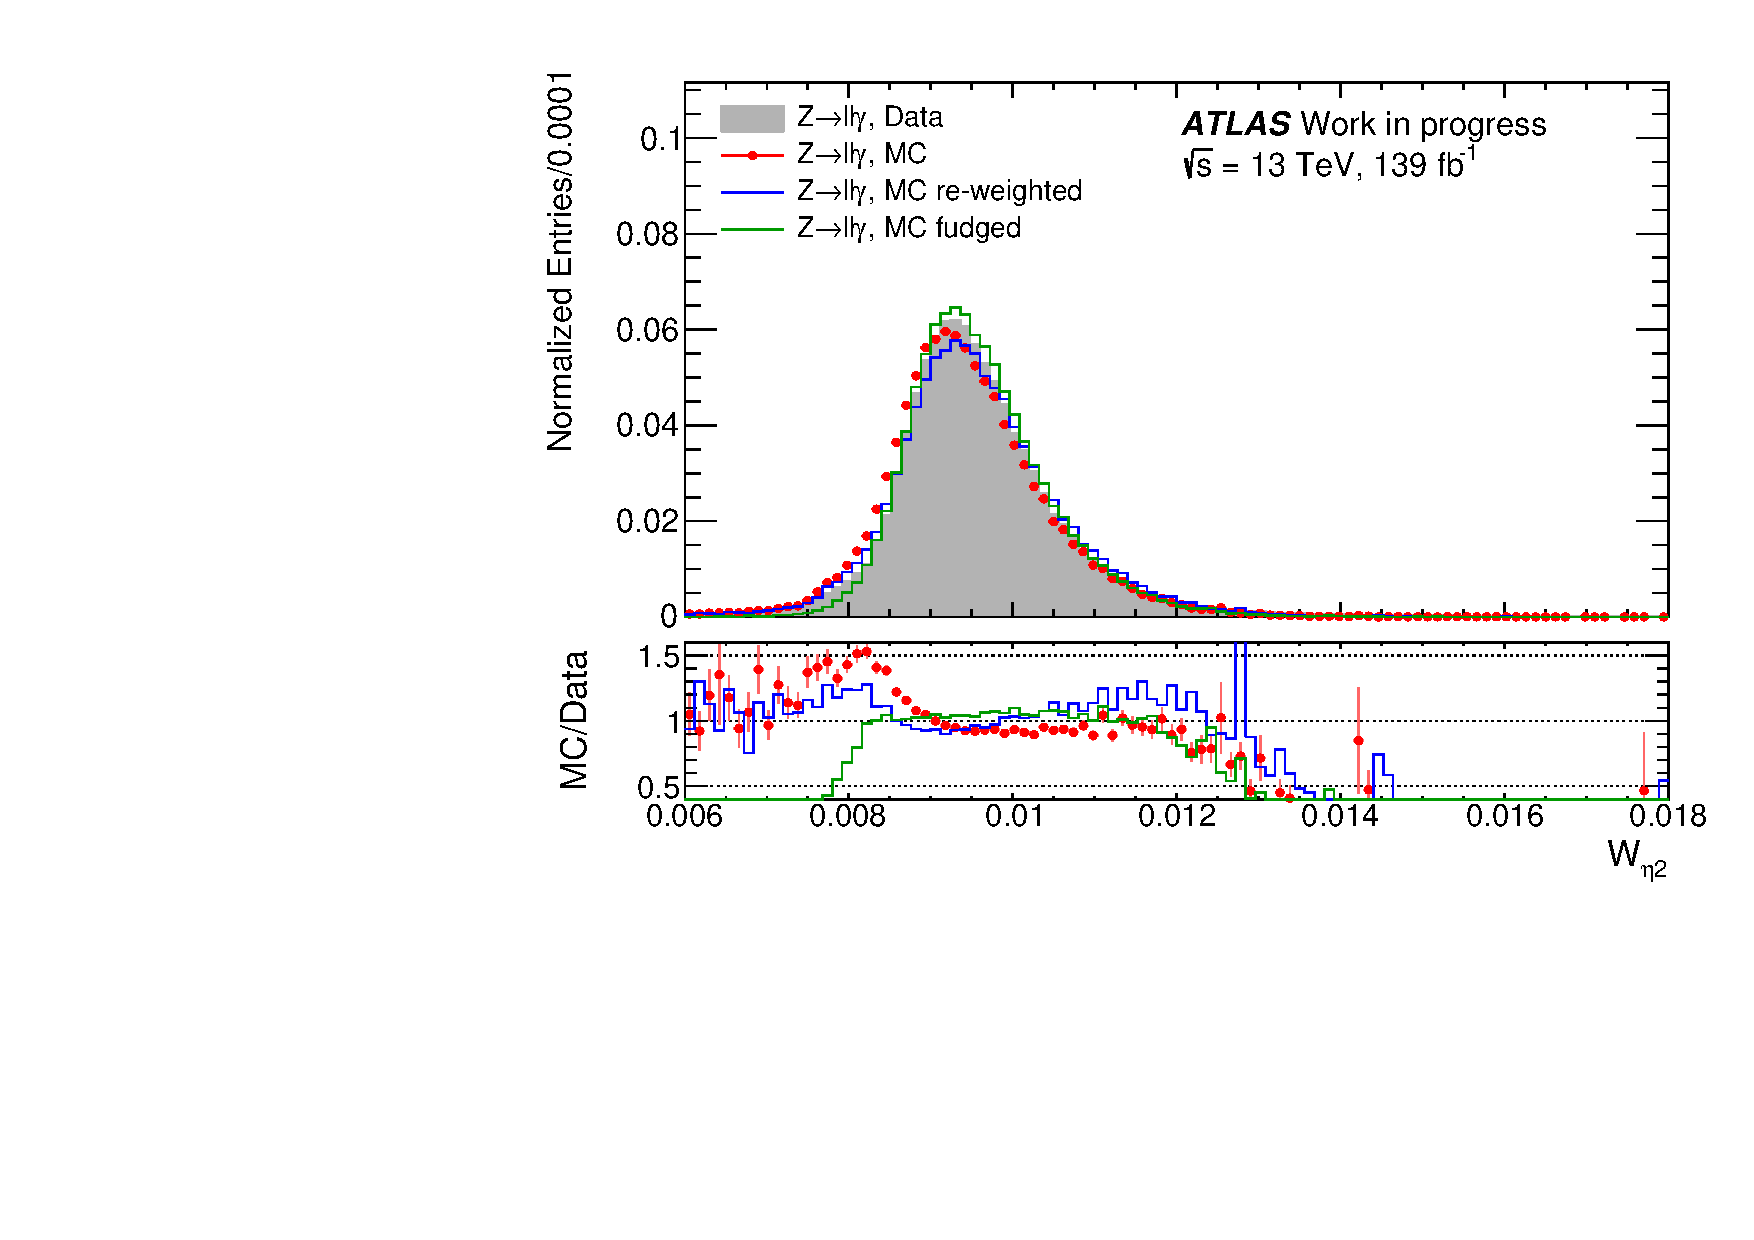
\includegraphics[width=\linewidth]{4_photonid/cell_rw/results/ss/c__u_eta00__ss_Weta2}
        \caption{\weta, unconverted photons}
    \end{subfigure}\\
    \begin{subfigure}[h]{0.32\linewidth}
        \centering
        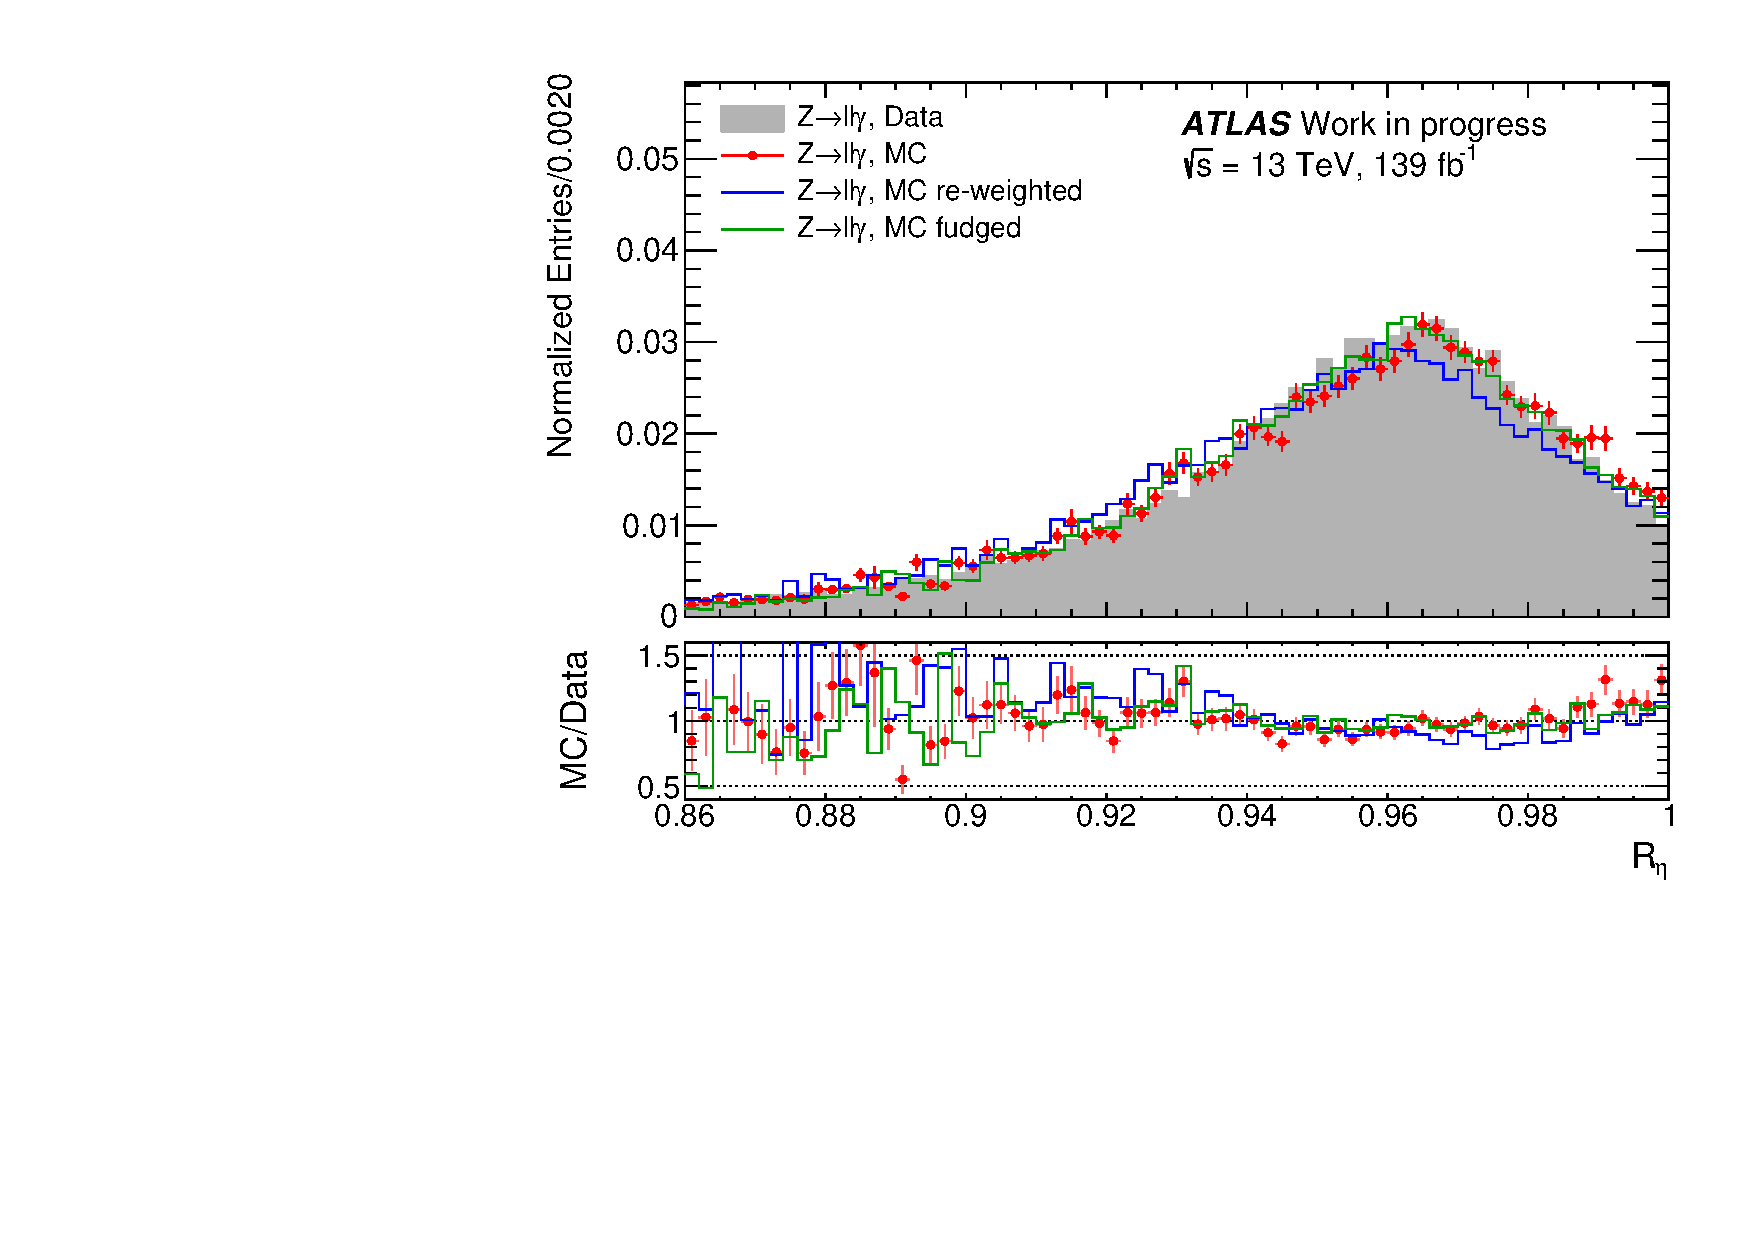
\includegraphics[width=\linewidth]{4_photonid/cell_rw/results/ss/c__c_eta00__ss_Reta}
        \caption{\reta, converted photons}
    \end{subfigure}
    \hfill
    \begin{subfigure}[h]{0.32\linewidth}
        \centering
        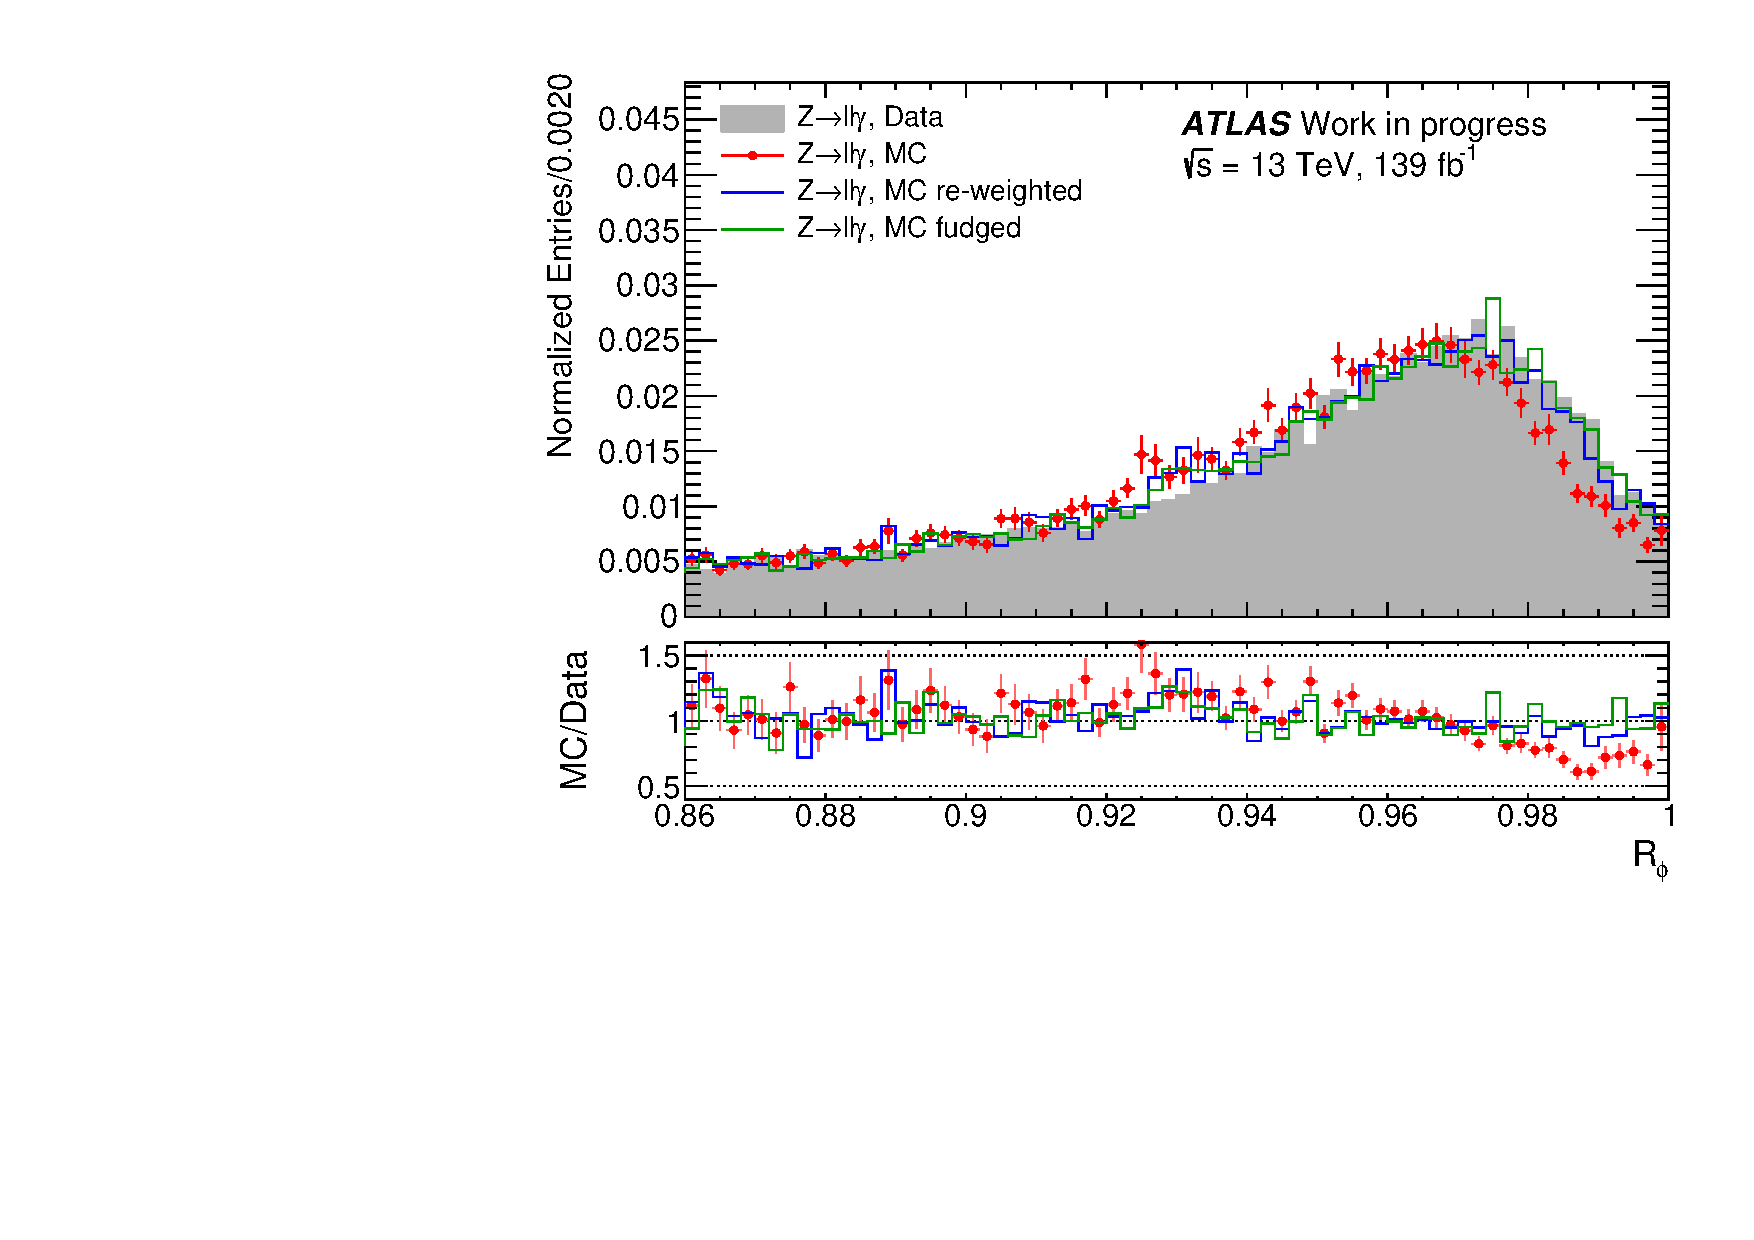
\includegraphics[width=\linewidth]{4_photonid/cell_rw/results/ss/c__c_eta00__ss_Rphi}
        \caption{\rphi, converted photons}
    \end{subfigure}
    \begin{subfigure}[h]{0.32\linewidth}
        \centering
        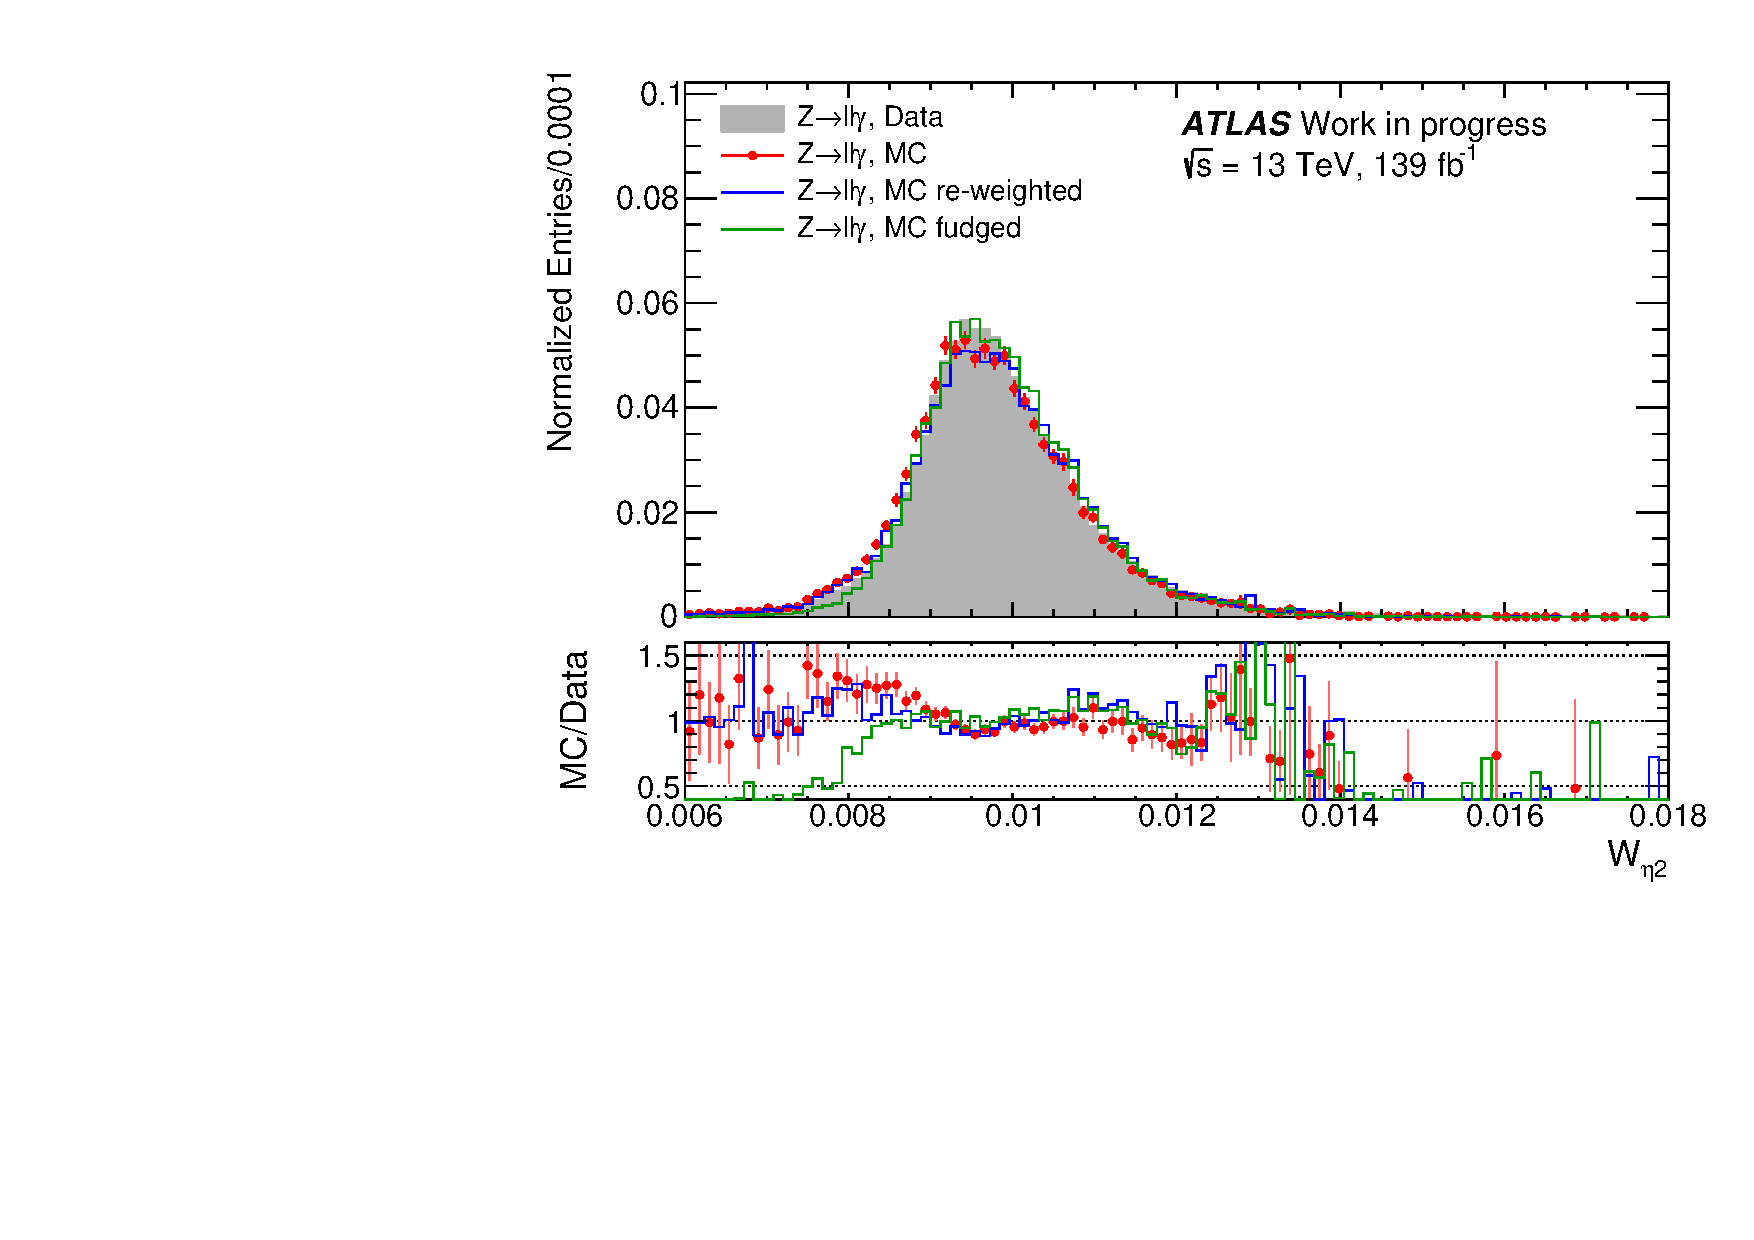
\includegraphics[width=\linewidth]{4_photonid/cell_rw/results/ss/c__c_eta00__ss_Weta2}
        \caption{\weta, converted photons}
    \end{subfigure}\\
    \caption{\acp{SS} distributions for unconverted (top row) and converted (bottom row) photons in \(\abseta<0.6\). Data is represented by the grey histogram. Uncorrected \ac{MC} simulation is shown with the red points and reweighted (fudged) \ac{MC} with the blue (green) line.}
    \label{fig:ss_corrections:cell_rw:results:ss}
\end{figure}






\section{Conclusions and future work}
\label{sec:ss_corrections:summary}

In the current chapter two methods to correct the observed disagreement between data and simulated \acfp{SS} were studied.

The \acf{FF} method has been historically used in the collaboration, which in the begginings it was only based on simple shifts of the distributions by adding a constant term to the variable. Even though the corrections led to good improvements and therefore obtaining \acfp{SF} closer to one, notable shape differences remained between data and simulation. In the context of this work, by adding a linear term to the variable transformation, the widths of the \ac{MC} distributions are fixed leading to even better agreement. This new method of correcting the \acp{SS} using \acp{FF} is referred as the shift+stretch method and is now used throughout the \ac{ATLAS} collaboration. 

A novel and lower-level method that aims to modify the energies in the \ac{ECAL} cells has also been developed. By using the energy distributions at each cell in clusters around the most energetic cell, it is possible to correct all the \acp{SS} at once. This method applies the same strategy of shifting and stretching the normalised energy from \ac{MC} simulation to match the distribution found in data. Although the method is new and still needs polishing and its extension to other layers of the \ac{ECAL}, it led to promising results in which some variables are corrected in the same way as with \acp{FF}. The cell-based energy reweighting method shows a great potential in the collaboration, not only in the context of \textit{offline} photon identification, but also at trigger level.

\subsection{Future work}

One of the most exciting and promising approaches to correct the \acp{SS} is the cell-based method. As previously mentioned, this approach could be employed on different steps on the photon identification process, such as at trigger level, or event \textit{offline} to correct all the \acp{SS} simultaneously. Another potential, and important usage, is to use the corrected clusters to directly compute photon identification, for example as considering the clusters as images and using a Convolutional Neural Network (CNN) to perform the photon identification~\cite{thesis_belfkir}.

\acfp{SSV} can be easily interpreted in terms of physical terms. For this reason, maintaining these physical quantities serve to understand the underlying physics of the processes. To continue correcting these variables is of great interest and there are several ways in which these can be achieved. The current method of transforming the variable but using higher-order terms remains a challenging task, but yet not explored. By making use of the novel Machine Learning (ML) techniques, it is possible to obtain correction factors for higher-order terms in the expansion, further correcting higher-order momenta of the distributions (skewness, kurtosis, etc.). Other interesting approach is using mulivariate reweighting, which was explored in \Refn{\cite{thesis_spah}}, showing very promising results.